\documentclass[10pt, letterpaper]{report}
% !TeX program = xelatex
%==================PREAMBOLO=======================%
\input{../../preamble/preamble.tex}
\usepackage{algorithm}
\usepackage{algpseudocode}
\newcommand{\titolo}{Artificial intelligence }

 %TOGLI COMMENTO SE USI XELATEX
%\usepackage{fontspec}
\title{\titolo} %========TITOLO========%
\author{Marco Casu}
\date{\vspace{-5ex}}
\begin{document}

%==================COPERTINA=======================%
\begin{titlepage}
    
\begin{center}
    %TOGLI COMMENTO SE USI XELATEX
   %\setmainfont{Palace Script MT}
   \HUGE Marco Casu\acc
\end{center}
\thispagestyle{empty}
\begin{figure}[h]
    \centering{
        %l'immagine deve avere una risoluzione 2048x2048
        \includegraphics[width=1\textwidth ]{images/Copertina.png}
    }
\end{figure}
\vfill 
\centering \includegraphics[width=0.4\textwidth ]{../../preamble/Stemma_sapienza.png} \acc
\centering \Large \color{sapienza}Faculty of Information Engineering, Computer Science and Statistics\\
Department of Computer, Control and Management Engineering\\
Master's degree in Artificial Intelligence and Robotics
\end{titlepage}

%===================FINE COPERTINA======================%
\newpage
%\pagecolor{cartaRiciclata}%\setmainfont{Algerian}
\Large
This document summarizes and presents the topics for the \titolo course for the Master's degree in Artificial Intelligence and Robotics at Sapienza University of Rome. The document is free for any use. If the reader notices any typos, they are kindly requested to report them to the author.
\vfill
\begin{figure}[h!]
    \raggedright
    \includegraphics[width=0.4\textwidth,right ]{../../preamble/tomodachi.pdf} 
\end{figure}
\newpage %\setmainfont{Times New Roman}
\normalsize

\tableofcontents 
\newpage

%==================FOOTER e HEADER=======================%
\fancyhf{}
\fancyhead[L]{\nouppercase{\leftmark}}
\fancyhead[R]{Section \thesection}
\fancyfoot[C]{\thepage}
\fancyfoot[L]{\titolo}
\fancyfoot[R]{ Marco Casu}
%\fancyfoot[R]{\setmainfont{Palace Script MT}\huge Marco Casu \setmainfont{Times New Roman}}
%==================FOOTER e HEADER=======================%
\newtheorem{definition}{Definition}
\newtheorem{theorem}{Theorem}
\newtheorem{proposition}{Proposition}
\newtheorem{lemma2}{Lemma}
\newtheorem{corollary}{Corollary}
%==================INIZIO======================%
\chapter{Introduction}
\section{Basic Definitions}
In the context of the artificial intelligence, an \textbf{agent} is an entity that can\begin{itemize}
    \item Perceive the environment through \textit{sensors} (percepts)
    \item Act upon the environment through \textit{actuators} (actions).
\end{itemize}
We say that an agent is \textbf{rational} if he selects the action that maximize a given \textit{performance measure}, informally, he attempts to do ''the right thing''. The best case is hypothetical and often unattainable, because the agent usually can't perform all the actions needed, and can't perceive all the information about the environment.\bigskip

An agent has a performance measure $M$ and a set $A$ of all possible actions, given percept a sequence $A$ and knowledge $K$ (data), he has to select the next action $a\in A$, is a map\begin{equation}
    M\times P\times K \longrightarrow A.
\end{equation} 
An action $a$ is optimal if it maximize the expected value of $M$, given the sequence $P$ and the knowledge $K$. An agent is rational if he always chooses the optimal action. More specifically, an agent consists in two components:\begin{itemize}
    \item an architecture which provides an interface to the environment
    \item a program executed on that architecture.
\end{itemize}
There are some limitation that we aren't considering, such as the fact that determining the optimal choice could take too much time or memory on the architecture.

\subsection{Types of Agents}
There are different kinds of agents, a \textbf{Table Driven Agent} is the simplest form of agent architecture. It's essentially a look-up table that maps every possible sequence of percepts (what the agent has sensed so far) to a corresponding action the agent should take. His behavior can be resumed in the algorithm \ref{alg:table_agent}.

\begin{algorithm}
    \caption{Table Driven Agent}\label{alg:table_agent}
    \begin{algorithmic}
    \Require \textit{percepts}
    \State \textbf{persistent}: \textit{percepts}, a sequence, initially empty
    \State\hphantom{persistent: .} \textit{table}, a table of actions, indexed by percept sequences, initially fully specified
    \State append \textit{percept} to the end of \textit{percepts} 
    \State \textit{action}$\leftarrow$\texttt{LookUp}(\textit{percepts,table})
    \State\Return \textit{action}
    \end{algorithmic}
\end{algorithm}
\bigskip


A \textbf{Reflex Agent} consists in three components:\begin{itemize}
    \item sensors to get information from the environment
    \item a decision making process, in form of a \textit{condition-action rules}, typically looks like \texttt{IF (condition) THEN (action)}.
    \item actuators, the outputs that allow the agent to affect or change the environment.
\end{itemize}

\begin{figure}[h!]
    \centering
    \includegraphics[width=0.4\textwidth ]{images/reflexAgent.png}
    \caption{Reflex agent diagram}
\end{figure}\bigskip

A \textbf{Model-Based Reflex Agent} is an enhanced version of the previous one, the key enhancement here is the inclusion of an \textit{Internal State} and a \textit{Model of the World} to make up for the agent's limited view of the environment. The internal state cannot simply be the last thing the agent saw; it needs to be updated to reflect reality. This is done using a Model of the World, which contains two key pieces of knowledge:\begin{itemize}
    \item 
    How the world evolves independently of the agent, his accounts for changes in the environment that occur regardless of the agent's actions (e.g., a clock ticking, an external event).
    \item
    How the agent's own actions affect the world, this is the effect of the agent's previous action (e.g., if the agent drove forward, its position changed).
\end{itemize}

\begin{figure}[h!]
    \centering
    \includegraphics[width=0.4\textwidth ]{images/ModelreflexAgent.png}
    \caption{Model Based Reflex agent diagram}
\end{figure}\bigskip

If a model based reflex agent consider the future prospective, is a \textbf{Goal Based Agent}, as shown in figure \ref{img:goal_agent}.

\begin{figure}[h!]
    \centering
    \includegraphics[width=0.4\textwidth ]{images/goal.png}
    \caption{Goal Based agent diagram}
    \label{img:goal_agent}
    \includegraphics[width=0.4\textwidth ]{images/utility.png}
    \caption{Utility Based agent diagram}
\end{figure}\bigskip

A \textbf{Utility Based Agent} is equipped with a \textit{utility function} that maps a state to a number which represents how
desirable the state is. Agent’s utility function is an internalization of the performance function.\bigskip

A \textbf{Learning Agent} is an architecture designed to improve its efficiency over time by separating four functions:\begin{itemize}
    \item  the performance element selects actions\item  
     the critic provides feedback on those actions against a standard\item   the learning element uses this feedback to update the agent's internal knowledge\item   the problem generator suggests exploratory actions to gain new knowledge. This structure enables the agent to continuously adapt and improve its decision-making.
\end{itemize}

\begin{figure}[h!]
    \centering
    \includegraphics[width=0.4\textwidth ]{images/learn_agent.png}
    \caption{Learning agent diagram}
\end{figure}\bigskip

An agent can be classified in one of the following groups:\begin{itemize}
    \item a \textbf{domain specific agent }  is a solver specific to a particular problem (such as playing chess), is usually more efficient.
    \item a \textbf{general agent} is a solver for general problems, such as learning the rule of any board game, is usually more intelligent but less efficient.
\end{itemize}
\subsection{The Environment}
An environment can be classified in terms of different attributes:\begin{itemize}
    \item An environment can be \textbf{fully observable} if all the relevant information are accessible to the sensors, otherwise is \textbf{partially observable}.
    \item If there are no uncertainty, the environment is \textbf{deterministic}. An environment is \textbf{stochastic} if uncertainty is quantified by using probabilities, otherwise is \textbf{non deterministic} if uncertainty is managed as actions with multiple outcomes.
    \item An environment is \textbf{episodic} if the correctness of an action can be evaluated instantly, otherwise if are evaluated in the future developments, is \textbf{sequential}. 
    \item An environment can be \textbf{static} or \textbf{dynamic}, if itdoes not change, but the agent's performance
score changes, the environment is called \textbf{semi-dynamic}.
    \item An environment can be perceived as \textbf{discrete} or \textbf{continuous}.
    \item In a single environment there may be multiple agent, that can be \textbf{competitive} or \textbf{cooperative}.
\end{itemize}
Many sub-areas of AI can be classified by:\begin{itemize}
    \item Domain-specific vs. general.
    \item The environment.
    \item Particular agent architectures sometimes also play a role, especially
    in Robotics.
\end{itemize}
It follows a classification of some areas in terms of the attributes we discussed:\begin{itemize}
    \item \textbf{Classical Search}, the environment is\begin{itemize}
        \item fully observable
        \item deterministic
        \item static 
        \item sequential
        \item discrete
        \item single-agent
    \end{itemize}
    and the approach is \textit{domain specific}.
    \item \textbf{Planning}, the environment is\begin{itemize}
        \item fully observable
        \item deterministic
        \item static
        \item sequential 
        \item discrete
        \item single-agent
    \end{itemize}
    and the approach is \textit{general}.
    \item \textbf{Adversarial Search}, the environment is\begin{itemize}
        \item fully observable
        \item deterministic
        \item static 
        \item sequential    
        \item discrete
        \item multi-agent
    \end{itemize}
    and the approach is \textit{domain specific}.
    \item \textbf{General Game Playing}, the environment is\begin{itemize}
        \item fully observable
        \item deterministic
        \item static 
        \item sequential    
        \item discrete
        \item multi-agent
    \end{itemize}
    and the approach is \textit{general}.
    \item \textbf{Constraint Satisfaction \& Reasoning}, the environment is\begin{itemize}
        \item fully observable
        \item deterministic
        \item static 
        \item episodic    
        \item discrete
        \item single-agent
    \end{itemize}
    and the approach is \textit{general}.
    \item \textbf{Probabilistic Reasoning}, the environment is\begin{itemize}
        \item partially observable
        \item stochastic
        \item static 
        \item episodic    
        \item discrete
        \item single-agent
    \end{itemize}
    and the approach is \textit{general}.
\end{itemize}
\chapter{Search Problems}
\section{Classical Search}
Let's consider two basic example of classical search problems, the first one is the following:\begin{center}
    \includegraphics[width=0.5\textwidth ]{images/map_search.png}
\end{center}
Starting from Zurigo, we would like to find a route to Zagabria. We have an initial state (Zurigo), and we have to apply actions (drive) to reach the goal state (Zagabria). Another example is the following, we want to solve the tiles-puzzle game, shown in figure \ref{img:tiles}, to reach the left state, starting from the right one, the actions to perform is the move of the tiles. A performance measure could be to minimize the summed-up action costs.

\begin{figure}[h!]
    \centering
    \includegraphics[width=0.6\textwidth ]{images/tile.png}
    \caption{The tile game}
    \label{img:tiles}
\end{figure}

In the classical search context, we restrict the agent's environment to a very simple setting, with a finite number of states and actions, a single agent and a fully observable state environment that doesn't evolve, given that assumption, the classical search problems are the simplest one, despite that, are very important problems in practice.\bigskip

\noindent Every problem specifies a state space.

\begin{definition}
    A \textbf{State Space} is a 6-tuple $\Theta=(S,A,c,T,I,S^G)$ where:\begin{itemize}
        \item $S$ is a finite set of the \textit{states}.
        \item $A$ is a finite set of \textit{actions}.
        \item $c:A\rightarrow\R^+$ is the \textit{cost function}.
        \item $T\subseteq S\times A\times S $ is the \textit{transition relation}, that describes how an action on a given state make the agent evolve to the next state. We assume that the problem is deterministic, so for all $s\in S$, $a\in A$, if $(s,a,s')\in T$ and $(s,a,s'')\in T$ then $s'=s''$.
        \item $I\in S$ is the \textit{initial state}
        \item $S^G\subseteq S$ is the set of the \textit{goal states}, where we want to end.
    \end{itemize}
\end{definition}
A transition $(s,a,s')$ can be denoted $s \xrightarrow{a} s'$, we say that $s\rightarrow s'$ if $\exists a$ such that $(s,a,s')\in T$ . We say that $\Theta$ has \textit{unit costs} if $\forall a\in A, \ \ c(a)=1$. A state space can be illustrated as a directed labeled graph. \begin{definition}
    Let $\Theta=(S,A,c,T,I,S^G)$ to be a state space, we say that\begin{itemize}
        \item $s'$ is a \textbf{successor} of $s$ if $s\rightarrow s'$
        \item $s'$ is a \textbf{predecessor} of $s$ if $s'\rightarrow s$
        \item we say that $s'$ is \textbf{reachable from} $s$ if\begin{align}
            &\exists (a_1\dots, a_n)\subseteq A\\
            &\exists (s_2\dots, s_{n-1})\subseteq S\\
            &(s,a_1,s_2)\in T\\
            &(s_2,a_2,s_3)\in T\\
            \vdots \\
            &(s_{n-1},a_n,s')\in T 
        \end{align}
        we can write the sequence as follows\begin{equation}
            s\xrightarrow{a_1}s_2,\dots, s_{n-1}\xrightarrow{a_n}s'.
        \end{equation}
        \item We say that $s$ is \textbf{reachable} (without reference state) if is reachable from $I$.
        \item $s$ is \textbf{solvable} if there exists $s'\in S^G$ such that $s'$ is reachable from $s$, otherwise $s$ is \textbf{dead end}.
    \end{itemize}
\end{definition}
\begin{definition}
    Let $\Theta=(S,A,c,T,I,S^G)$ to be a state space, and let $s\in S$. A \textbf{solution} for $s$ is a path from $s$ to some goal state $s'\in S^G$. The solution is \textbf{optimal} if it's cost is minimal, let $H$ to be the set of all possible solution (sequence of states) for $s$\begin{equation}
        H=\{\text{paths from }s\text{ to }s'\in S^G\}=\{(s_{i0},s_{i1},s_{i1},\dots s_{in})  : s_{in}\in S^G, \ s_{i0}=s\}
    \end{equation}
    where $n^i$ is the length of the $i$-th solution.
    The optimal solution is\begin{equation}
        \arg \min_{(s,s_{i1},\dots s_{in})\in H}\sum_{j=0}^{n^i} c(s_{ij}).
    \end{equation}
\end{definition}
A solution for $I$ is called \textbf{solution for $\Theta$}, if such that solution exists, $\Theta$ is \textbf{solvable}.
\subsection{Vacuum Cleaner Example}
Let's consider a vacuum cleaner, that is the agent of our problem, the goal is to clean a room, the vacuum cleaner can be in two possible points (left and right), this points can be clean or dirty. The agent can perform the following actions\begin{itemize}
    \item move right 
    \item move left 
    \item suck the dust on the floor
\end{itemize}
there are 8 possible states\begin{itemize}
    \item left point clean, right point clean, vacuum cleaner is on right point
    \item left point dirty, right point clean, vacuum cleaner is on right point
    \item left point clean, right point dirty, vacuum cleaner is on right point
    \item left point dirty, right point dirty, vacuum cleaner is on right point
    \item left point clean, right point clean, vacuum cleaner is on left point
    \item left point dirty, right point clean, vacuum cleaner is on left point
    \item left point clean, right point dirty, vacuum cleaner is on left point
    \item left point dirty, right point dirty, vacuum cleaner is on left point
\end{itemize}
the initial state is the one with the left point dirty, right point dirty, and the vacuum cleaner on the left point, we denote the actions $R$ (move right), $L$ (move left), $S$ suck. The state space of the problem is show in figure \ref{img:vacuum_cleaner}. 

\begin{figure}[h!]
    \centering
    \includegraphics[width=0.6\textwidth ]{images/vacuum.png}
    \caption{The vacuum cleaner state space}
    \label{img:vacuum_cleaner}
\end{figure}
Some example of set of actions that can lead from the initial state to a goal state are\begin{align*}
    &S\longrightarrow R\longrightarrow S\\
    &S\longrightarrow R\longrightarrow R\longrightarrow S\\
    &R\longrightarrow S\longrightarrow L\longrightarrow S
\end{align*}

Typically, the state space is exponentially large in the size of its specification, search problems are typically computationally hard and/or $\mathsf{NP}$-complete. We say that we can give an \textit{explicit description} of a search problem if we can define his state space as a graph.
\section{Problem Descriptions}
\begin{definition}
    We have a \textbf{black box description} of the problem if we can't describe the state space explicitly but we can\begin{itemize}
        \item Know which is the initial state
        \item Check if a given state is a goal state
        \item Check the cost of a given action $a$
        \item Given a state $s$, check all the actions that are applicable to state $s$
        \item Given a state $s$ and an applicable action $a$, we can get the successor state.
    \end{itemize}
\end{definition}
We can think about it in a programming-way, given a problem described by $\Theta=(S,A,c,T,I,S^G)$, we can't check directly $\Theta$, but we have an \textit{API} of the problem that provide the following functions \begin{itemize}
    \item \texttt{InitialState()} : return the initial state of the problem
    \item \texttt{GoalTest($s$)} : return true if and only if $s\in S^G$
    \item \texttt{Cost}($a$ : return $c(a)$)
    \item \texttt{Actions}($s$) : return the set $\{ a \ : \ \exists  s\xrightarrow{a} s'\in T \text{ for some }s'\in S\}$
    \item \texttt{ChildState}($s,a$) : return $s'$ if $s\xrightarrow{a} s'\in T$.
\end{itemize}
We \textbf{specify} a search problem if we can program/access to such an \textit{API}. There are a declarative description too.
\begin{definition}
\end{definition}
We have a \textbf{declarative description} of the problem if is described by the following sets:\begin{itemize}
    \item $P$ is a set of boolean variables (\textit{propositions})
    \item $I\subseteq P$ is the subset of $P$ indicating which propositions are true in the initial states.
    \item $G\subset P$ is the subset of $P$ describing the goal states in the following way\begin{itemize}
        \item a state $s$ is a set of propositions 
        \item $s\subseteq G \iff s$ is a goal state
    \end{itemize}
    \item $A$ is a set of actions, each action $a$ is described by\begin{itemize}
        \item a set $pre_a\subseteq P$ of \textit{precondition}, $a$ can be performed if and only if the conditions in $pre_a$ are true.
        \item a set of propositions $add_a$
        \item a set of propositions $del_a$
        \item the outcome of each action is the state $(\{s\}\cup add_a )\backslash del_a$
        \item $c:A\rightarrow\R$ is the cost function.
    \end{itemize}
\end{itemize}
Declarative descriptions are strictly more powerful than black box ones. In this section we assume the black box description. In principle, the search strategies we will discuss can be used with any
problem description that allows to implement the black box \textit{API}.
\subsection{Missionaries and Cannibals Example}
The problem is the following\begin{itemize}
    \item there are a river and a boat that can carry the people from the left bank to the right 
    \item there are 6 people, 3 missionaries and 3 cannibals 
    \item the boat can carry 0, 1 or 2 people at the same time, not 3 
    \item the goal is to get  everybody to the left bank
    \item if at any time, there are more cannibals than missionaries in one bank, the missionaries get killed and the game is lost. 
\end{itemize}
We can model the problem as follows\begin{itemize}
    \item the state space $S$ is \begin{equation}
        S=\{(M,C,B) \ : \ M+C=6, \ 0\le M \le 3, \ 0\le C \le 3, \  B\in\{0,1\}\}
    \end{equation}
    $M$ represents the current number of missionaries on the right bank, $S$ represents the current number of cannibals on the right bank, $B=1$ if the boat is on the right bank, otherwise is on the left.
    \item the initial state is $(3,3,1)$
    \item the goal states are $S^G={(0,0,0),(0,0,1)}$
    \item each actions have the same cost, is negligible
    \item the action that can be performed are the following\begin{itemize}
        \item if $B=1$, we can subtract (in total) 1 or 2 from $M$ or $C$ (or both), and set $B=0$.
        \item if $B=0$, we can add (in total) 1 or 2 from $M$ or $C$ (or both), and set $B=1$.
    \end{itemize}
    an action is applicable if and only if the following condition are satisfied after\begin{itemize}
        \item $M\ge C$ if $M>0$, this decode the facts that the cannibals can't be more or equals than the missionaries on the right bank if there are missionaries on the left bank
        \item if $M<3$ (some missionaries are on the left bank) then $(3-M)>(3-C)$ the missionaries on the left bank must be greater then the cannibals on the left bank.
    \end{itemize}
\end{itemize}
To search a solution we can start from the initial state and expand the tree of possible solutions accordingly to the applicable actions.\begin{center}
    \includegraphics[width=0.5\textwidth ]{images/missionaries.eps}
\end{center}
\subsection{Tree and Graph Search}
In the search context the following terminology is used
\begin{itemize}
    \item Search node $n$: Contains a state reached by the search, plus information about how it was reached.
    \item Path cost $g(n)$: The cost of the path reaching $n$.
    \item Optimal cost $g^*$: The cost of an optimal solution path. For a state $s$, $g^*(s)$ is the cost of a cheapest path reaching $s$.
    \item Node expansion: Generating all successors of a node, by applying all actions applicable to the node's state $s$. Afterwards, the state $s$ itself is also said to be expanded.
    \item Search strategy: Method for deciding which node is expanded next.
    \item Open list: Set of all nodes that currently are candidates for expansion. Also called frontier.
    \item Closed list: Set of all states that were already expanded. Used only in graph search, not in tree search (up next). Also called explored set.
\end{itemize}
When we explore the state space of a problem we can maintain a closed list of all the node that has been already searched, to check for each generated new node if is already in the list (if so, we discard it). If such list is used, the search is called \textbf{graph search}, else, if the same state may appear in many search nodes, is called \textbf{tree search}. The tree search doesn't use a list so it require less memory.\bigskip

When we analyze a search algorithm, we are interested in various properties\begin{itemize}
    \item \textbf{Completeness}: the algorithm is guaranteed to find a solution (it there are one).
    \item \textbf{Optimality}: the returned solution is guaranteed to be optimal. 
    \item \textbf{Time Complexity}: How long does it take to find a solution? (Measured
in generated states).
    \item \textbf{Space Complexity}: How much memory does the search require?
(Measured in states).
    \item \textbf{Branching Factor}: The number $b$ of how many successor a state may have.
    \item \textbf{Gal depth}: the number $d$ of action required to reach the shallowest (nearest to the initial state) goal state.
\end{itemize}
\section{Blind Search}
We talk about \textit{blind search} if the problem does not require any input beyond the problem API. Does not require any additional work from the programmer. For each node $n$ in the search context, we define the following data structure:\begin{itemize}
    \item $n$.State is the state which te node contains 
    \item $n$.Parent is node in the search tree that generated this node
    \item $n$.Action is the action that was applied to the parent to generate the node
    \item $n$.PathCost, also denoted $g(n)$, is the cost of the path from the initial state to the node (as indicated by the parent pointers).
\end{itemize}
On a node we can perform the following operations\begin{itemize}
    \item Solution($n$) returns the path from the initials state to $n$
    \item ChildNode($n,a$) returns the node $n$ corresponding to the application of action $a$ in state $n$.State. 
\end{itemize}
We also have the open list (called frontier) where we can perform the following actions:\begin{itemize}
    \item Empty?(frontier) returns true if and only if there are no more elements in the
open list.
    \item Pop(frontier) returns the first element of the open list, and
removes that element from the list.
    \item Insert(element,frontier) inserts an element into the open list.
\end{itemize}
The insert function can put the element in front, in the last positions, or in other positions, it depends from the implementation (different implementations yield different search strategies).
\subsection{Breadth-First Search}
The strategy is to expand nodes in the order they were produced, as a FIFO queue, we expand the shallowest unexpanded node.
\begin{center}
    \includegraphics[width=1\textwidth ]{images/bfs.png}
\end{center}
This algorithm \ref{alg:BFS} is complete and optimal (in case of unit cost function). We are using the black box \textit{API}.

\begin{algorithm}
    \caption{Breadth-First Search}\label{alg:BFS}
    \begin{algorithmic}
    \Require $problem$
    \State $node\leftarrow$\texttt{InitialState()}
    \If{\texttt{GoalTest($node$.State)}}
    \State\Return Solution($node$)
    \EndIf
    \State $frontier\leftarrow$ a FIFO queue with $node$ in it
    \State $explored\leftarrow$ an empty set
    \While{true}
    \If{Empty?($frontier$)}
    \State\Return Failure
    \EndIf
    \State $node\leftarrow$pop($frontier$)
    \State add $node$.State in $explored$
    \For{each $action$ in \texttt{Actions($node$.State)}}
    \State $child\leftarrow$ChildNode($node,action$)
    \If{$child$.State is not in $explored$ or $frontier$}
    \If{\texttt{GoalTest($child$.State)}}
    \State\Return Solution($child$)
    \EndIf
    \State $frontier\leftarrow$Insert($child$,$frontier$)
    \EndIf
    \EndFor
    \EndWhile
    \end{algorithmic}
\end{algorithm}
Let $b$ to be the maximum branching factor and $d$ the depth of the shallowest goal state, an upper bound (in the worst case) for the number of nodes generated (time complexity) is\begin{equation}
    b+b^2+b^3\dots +b^d\in O(b^d)
\end{equation}
the same for the space complexity since  all generated nodes are kept in memory. Let's see an example, assume that $b=10$, the agent can generate $10^4$ nodes per second, and each node has a size of $1$ kilobyte, we have the following data:\begin{center}
    \begin{tabular}{|c|c|c|c|}
        \hline
        \textbf{Depth} & \textbf{Nodes} & \textbf{Time} & \textbf{Memory} \\
        \hline
        2 & 110 & 0.11 milliseconds & 107 kilobytes \\
        \hline
        4 & 11,110 & 11 milliseconds & 10.6 megabytes \\
        \hline
        6 & $10^6$ & 1.1 seconds & 1 gigabyte \\
        \hline
        8 & $10^8$ & 2 minutes & 103 gigabytes \\
        \hline
        10 & $10^{10}$ & 3 hours & 10 terabytes \\
        \hline
        12 & $10^{12}$ & 13 days & 1 petabyte \\
        \hline
        14 & $10^{14}$ & 3.5 years & 99 petabytes \\
        \hline
    \end{tabular}
\end{center}
The critical resource for this method is the memory.
\subsection{Depth-First Search}
The strategy is to expand the most recent explored node, as a LIFO queue, we expand the deepest unexpanded node. 
\begin{center}
    \includegraphics[width=0.7\textwidth ]{images/dfs.png}
\end{center}
The algorithm is not complete since it may take infinite time, since there is no check for cycles along the branches. It's not optimal since he chooses a direction and looks for a path to a goal state. Is typically implemented as a recursive function, as in algorithm \ref{alg:DFS}.\bigskip

\begin{algorithm}
    \caption{Depth-First Search}\label{alg:DFS}
    \begin{algorithmic}
    \Require $problem$, a node $n$
    \If{\texttt{GoalTest}($n$.\texttt{State})}
    \State\Return empty action sequence
    \EndIf
    \For{each $action$ in \texttt{Actions}($node$.\texttt{State})}
    \State $n'\leftarrow$ChildNode($node$,$action$)
    \State result$\leftarrow$Depth-First Search($problem$,$n'$)
    \If{result$\ne$ failure}
    \State\Return $action \ \circ$ result
    \EndIf
    \EndFor
    \State\Return failure
    \end{algorithmic}
\end{algorithm}

\noindent With $action \ \circ$ result is denoted the concatenation of actions. 
About the space complexity, this methods stores only a single path of actions, from the root to a leaf node, since once a
 node has been expanded, it can be removed from memory as soon as all its
 descendants have been fully explored.

 If $m$ is the maximal depth reached, the space occupied is in $O(bm)$. About the time complexity, in the worst case the nodes generated is in $O(b^m)$.
 \subsection{Uniform-Cost Search}
 This methods is equivalent to the well known Dijkstra's algorithm. We expand the node with the lowest path cost $g(n)$, the frontier is ordered by the path cost, with the lowest first. It differs from the BFS since a test is added to check if a better path is found to a node currently
 on the frontier.

 \begin{algorithm}
    \caption{Uniform-Cost Search}\label{alg:DFS}
    \begin{algorithmic}
    \Require $problem$
    \State $node\leftarrow$\texttt{InitialState()}
    \State $frontier\leftarrow$ priority queue ordered by ascending $g$
    \State $explored\leftarrow$ empty set of states
    \While{true}
    \If{Empty?($frontier$)}
    \State\Return failure 
    \EndIf
    \State $n\leftarrow$Pop($frontier$)
    \If{\texttt{GoalTest}($n$.State)}
    \State\Return Solution($n$)
    \EndIf
    \State$explored\leftarrow explored\cup n$.State
    \For{each $action$ in \texttt{Actions}($node$.\texttt{State})}
    \State $n'\leftarrow${ChildNode}($n$,$a$)
    \If{$n'$.State$\notin explored\cup$States($frontier$)}
    \State $frontier\leftarrow$insert($n'$,$frontier$)
    \Else{ \textbf{if} $\exists n''\in frontier \ : \ n''.$State=$n'$.State$ \land \ g(n')<g(n'')$}
    \State replace $n''$ with $n'$ in $frontier$
    \EndIf
    \EndFor
    \EndWhile
    \end{algorithmic}
\end{algorithm}
\begin{theorem}
    The Uniform-Cost search algorithm is optimal, since the Dijkstra's algorithm is optimal, and Uniform-cost search is equivalent to Dijkstra's algorithm on the state space graph. 
\end{theorem}

The algorithm is complete if we assume that, the costs are strictly positive and the state space is finite. The time and space complexity are\begin{equation}
    O(b^{1+\lfloor\nicefrac{g^*}{*}\rfloor})
\end{equation}where\begin{itemize}
    \item $g^*$ is the cost of an optimal solution 
    \item $\epsilon=\min c$ is the positive cost of the cheapest action, the minimum of the function $c$.
\end{itemize}
\subsection{Iterative Deepening Search}
This is an altered version of the Depth-First Search algorithm, where we define a predetermined depth limit, and apply the DFS in function of that limit, iteratively applying this by increasing the depth limit each time.
\begin{center}
    \includegraphics[width=0.7\textwidth ]{images/iterative_deep.png}
\end{center}
We split the algorithm in three different function.

 \begin{algorithm}
    \caption{Iterative Deepening Search}\label{alg:IDS}
    \begin{algorithmic}
    \Require $problem$
    \For{$depth=0,1\dots\infty$}
    \State $result\leftarrow$Depth Limited Search($problem$,$depth$)
    \If{$result\ne$cutoff} 
    \State\Return $result$
    \EndIf
    \EndFor
    \end{algorithmic}
\end{algorithm}

 \begin{algorithm}
    \caption{Depth Limited Search}\label{alg:DLS}
    \begin{algorithmic}
    \Require $problem,limit$
    \State $node\leftarrow$ \texttt{InitialState()}
    \State\Return Recursive DLS($node$,$problem$,$limit$)
    \end{algorithmic}
\end{algorithm}

The algorithm is complete since we are keep searching until a solution is found, is also optimal if all the cost are unitary, the space complexity is $O(bd)$. The time complexity is in $O(b^d)$, this methods combines the advantages of breadth-first and depth-first search. It is the preferred blind search method in large state spaces with unknown solution depth.\bigskip

 \begin{algorithm}
    \caption{Recursive DLS}\label{alg:EDLS}
    \begin{algorithmic}
    \Require $n,problem,limit$
    \If{\texttt{GoalTest($n$.State)}}
    \State\Return empty action sequence
    \EndIf
    \If{$limit$==0}
    \State\Return cutoff
    \EndIf
    \State $cutoffOccurred\leftarrow $false
    \For{each $action$ in \texttt{Actions}($node$.\texttt{State})}
    \State $n'\leftarrow$ChildNode($node$,$action$)
    \State result$\leftarrow$Recursive DLS($problem$,$n'$)
    \If{$result$==cutoff}
    \State $cutoffOccurred\leftarrow $true
    \Else
    \If{result$\ne$ failure}
    \State\Return $action \ \circ$ result
    \EndIf
    \EndIf
    \EndFor
    \If{$cutoffOccurred$}
    \State\Return cutoff 
    \EndIf
    \State\Return failure
    \end{algorithmic}
\end{algorithm}

The following table is a summary of the methods that we considered in this section, confronting the time and space complexity.\begin{center}
    \begin{tabular}{|c|c|c|c|c|c|}
\hline
Criterion                                                  & BFS                                                                 & \begin{tabular}[c]{@{}c@{}}Uniform\\ Cost\end{tabular}                                             & DFS      & \begin{tabular}[c]{@{}c@{}}Depth\\ Limited\end{tabular} & \begin{tabular}[c]{@{}c@{}}Iterative\\ Deeping\end{tabular}         \\ \hline
Completness                                                & \begin{tabular}[c]{@{}c@{}}Yes, if \\ $a$ is finite\end{tabular}    & \begin{tabular}[c]{@{}c@{}}Yes, if \\ $a$ is finite\\ and action costs \\ is positive\end{tabular} & No       & No                                                      & \begin{tabular}[c]{@{}c@{}}Yes, if \\ $a$ is finite\end{tabular}    \\ \hline
Optimality                                                 & \begin{tabular}[c]{@{}c@{}}Yes if action\\ costs are 1\end{tabular} & Yes                                                                                                & No       & No                                                      & \begin{tabular}[c]{@{}c@{}}Yes if action\\ costs are 1\end{tabular} \\ \hline
\begin{tabular}[c]{@{}c@{}}Time\\ Complexity\end{tabular}  & $O(b^d)$                                                            & $O(b^{1+\lfloor \nicefrac{g^*}{\epsilon} \rfloor})$                                                & $O(b^m)$ & $O(b^l)$                                                & $O(b^d)$                                                            \\ \hline
\begin{tabular}[c]{@{}c@{}}Space\\ Complexity\end{tabular} & $O(b^d)$                                                            & $O(b^{1+\lfloor \nicefrac{g^*}{\epsilon} \rfloor})$                                                & $O(bm)$  & $O(bl)$                                                 & $O(bd)$                                                             \\ \hline
\end{tabular}
\end{center}
where
\begin{itemize}
\item $b$: finite branching factor
\item $d$: goal depth
\item $m$: maximum depth of the search tree
\item $l$: depth limit
\item $g^*$ : optimal solution cost
\item $\epsilon>0$: minimal action cost.
\end{itemize}
\section{Informed Search}\label{InformedSearch}
\begin{definition}
    Let $\Pi$ to be a problem with $S$ the set of states, a \textbf{heuristic} $h$ is a function $$h:S\rightarrow\R^+\cup\{\infty,0\}$$ such that, if $s$ is a goal state, then $h(s)=0$.
\end{definition}
A heuristic function $h^*$ is perfect if $h^*(s)$ is exactly the cost of a cheapest path from $s$ to a goal state, and $h^*(s)=\infty$ if no such path exists. $h^*$ is also called the \textit{goal distance} of $s$.\bigskip

$h$ depend only on the state $s$ and not on the search node (the path taken to reach $s$ don't affect $h(s)$). If $n$ is a search node, we usually write $h(n)$ instead of $h(n.State)$ as an abuse of notation.

The purpose of $h$ is to estimate how far we are from a solution, clearly, some time is needed to calculate the value of $h$, ideally we would like a function $h$ that is very precise in the estimation, and which is quick to calculate, these two objectives are generally in conflict with each other.

Given a problem $\Pi$, a heuristic function $h$ for $\Pi$ can be
obtained as goal distance within a simplified (relaxed) problem $\Pi'$. A classic example is using Euclidean distance as a heuristic function in a graph representing points on a map.
 \begin{center}
    \includegraphics[width=0.7\textwidth ]{images/h_distance.png}
\end{center}
Another example is when we have to reach a goal in discrete grid with some ''pitfalls'' to avoid.
\begin{center}
    \includegraphics[width=0.7\textwidth ]{images/pitfalls_1.png}
\end{center}
in each cell is presented the value of the perfect heuristic $h^*$. A reasonable and accurate heuristic may be the Manhattan distance. 
\begin{center}
    \includegraphics[width=0.7\textwidth ]{images/pitfalls_2.png}
\end{center}
For some specific grid configurations this  heuristic might be inaccurate:
\begin{center}
    \includegraphics[width=0.7\textwidth ]{images/pitfalls_3.png}
\end{center}
\begin{definition}
    Let $h^*$ to be  a perfect heuristic. A heuristic $h$ is \textbf{admissible} if $\forall s\in S$ we have $h(s)\le h^*(s)$.
\end{definition}
An admissible heuristic function never overestimates the cost to reach the goal.\begin{definition}
    A heuristic $h$ is \textbf{consistent} if, for all transition $s\xrightarrow{a} s'$ in $\Theta$, we have $h(s)-h(s')\le c(a)$. 
\end{definition}
The consistency is important,  when applying an action $a$, the heuristic value cannot
 decrease by more than the cost of $a$.
 \begin{proposition}
    If $h$ is consistent then is admissible.
 \end{proposition}
 \textit{Proof}: The proof is done by induction.\begin{itemize}
    \item Base case: let $s$ to be the goal state, so $h(s)=h^*(s)=0$, so $h(s)\le h^*(s)$ trivially holds.
    \item Assume that the claim holds for all states $s'$ where the cheapest path to the goal state have length $n$. Let $s$ to be a state with goal length $n+1$, which have the first transition$$s\xrightarrow{a}s' $$ so\begin{eqnarray}
        h(s)\le h(s')+c(a)
    \end{eqnarray}
    by the inductive hypothesis:\begin{eqnarray}
        h(s')\le h^*(s')
    \end{eqnarray}
    by construction:\begin{equation}
        h^*(s)=h^*(s')+c(a)
    \end{equation}
    by combining the equations:\begin{eqnarray}
        \begin{cases}
            h(s)\le h(s')+c(a)\\
            h(s')\le h^*(s')\\ 
            h^*(s)=h^*(s')+c(a)
        \end{cases}\implies h(s)\le h^*(s)
    \end{eqnarray}
    \hfill$\blacksquare$
 \end{itemize}
 The Euclidean distance for the map-travel problem is consistent.
 \subsubsection{Systematic search vs. local search:}
\begin{itemize}
    \item \textbf{Systematic search strategies:} No limit on the number of search nodes kept in memory at any point in time.
    \begin{itemize}
        \item[$\rightarrow$] Guarantee to consider all options at some point, thus complete.
    \end{itemize}
    \item \textbf{Local search strategies:} Keep only one (or a few) search nodes at a time.
    \begin{itemize}
        \item[$\rightarrow$] No systematic exploration of all options, thus incomplete.
    \end{itemize}
\end{itemize}
\subsubsection{Tree search vs. graph search:}
\begin{itemize}
    \item For the systematic search strategies, we consider graph search algorithms exclusively, i.e., we use duplicate pruning.
    \item There are tree search versions of these algorithms. These are easier to understand, but aren't used in practice. (Maintaining a complete open list, the search is memory-intensive anyway.)
\end{itemize}
The informed search uses problem-specific knowledge, by using an evaluation function $f$ at each node, that function estimate the ''desirability'' of expanding that node, and we choose to expand the most desirable unexpanded node $$\arg\max_{\text{unexpanded }n} f(n).$$
We usually implement this with a sorted queue ordered based on the desirability of expansion, this queue is called \textbf{frontier}.
\subsection{Greedy Best-First Search}
We use the heuristic function $f$ as the evaluation function and we expand the node that is closest to the goal.
\begin{algorithm}
    \caption{Greedy Best-First Search}\label{alg:greedy-best-first}
    \begin{algorithmic}
    \Require A problem $\Pi$
    \State $n\leftarrow$ a node $n$ such that $n.State=\Pi.InitialState$
    \State $frontier\leftarrow$ a priority queue ordered by ascending $h$
    \State $explored\leftarrow $empty set of states
    \While{\textbf{True}}
    \State \textbf{If} $frontier$ is empty \textbf{Then Return} failure 
    \State $n\leftarrow Pop(frontier)$
    \State \textbf{If} $n.State$ is the goal state \textbf{Then Return} $Solution(s)$
    \State $explored\leftarrow explored \cup n.State$
    \For{each action $a$ in $\Pi.Actions(n.State)$}
    \State $n'\leftarrow ChildNode(\Pi,n,a)$
    \State \textbf{If} $n'.State\notin explored \cup States(frontier)$\textbf{ Then} $insert(n',h(n'),frontier)$ 
    \EndFor
    \EndWhile
    \end{algorithmic}
\end{algorithm}
This algorithm is complete thanks to the assumption that the state space is finite, but is not optimal, there exists an algorithm that is optimal and complete.
\subsection{The A* Algorithm}
A* is an informed search algorithm used for path finding and graph traversal. It finds the shortest path from a starting node to a target goal by combining the benefits of Dijkstra's algorithm and Greedy Best-First Search.


The core of A* is the evaluation function $f(n)$, which determines the priority of each node $n$ in the search frontier:
\[ f(n) = g(n) + h(n) \]
\begin{itemize}
    \item \textbf{$g(n)$ (The Path Cost):} The actual cost of the path from the start node to the current node $n$. This ensures the algorithm doesn't ignore the distance already traveled.
    \item \textbf{$h(n)$ (The Heuristic):} An estimated cost to get from node $n$ to the goal. This ''educated guess'' allows the algorithm to prioritize nodes that appear to lead directly toward the target.
    \item \textbf{$f(n)$ (The Total Estimated Cost):} The estimated cost of the cheapest solution passing through node $n$.
\end{itemize}


The algorithm maintains a \textbf{frontier} (priority queue) of nodes to be explored, ordered by ascending $f(n)$ values.
\begin{enumerate}
    \item It always expands the node with the \textbf{lowest $f(n)$} first.
    \item If $h(n)$ is \textit{admissible} (never overestimates the actual cost), A* is guaranteed to find the optimal (shortest) path.
    \item By balancing $g(n)$ and $h(n)$, A* avoids expanding paths that are already too expensive while remaining focused on the goal.
\end{enumerate}
\begin{algorithm}
    \caption{A*}\label{alg:A*}
    \begin{algorithmic}
    \Require A problem $\Pi$
    \State $n\leftarrow$ a node $n$ such that $n.State=\Pi.InitialState$
    \State $frontier\leftarrow$ a priority queue ordered by ascending $g+h$
    \State $explored\leftarrow $empty set of states
    \While{\textbf{True}}
    \State \textbf{if} $frontier$ is empty \textbf{Then Return} failure 
    \State $n\leftarrow Pop(frontier)$
    \State \textbf{if} $n.State$ is the goal state \textbf{Then Return} $Solution(s)$
    \State $explored\leftarrow explored \cup n.State$
    \For{each action $a$ in $\Pi.Actions(n.State)$}
    \State $n'\leftarrow ChildNode(\Pi,n,a)$
    \If{$n'.State\notin explored \cup States(frontier)$}
    \State $insert(n',h(n')+g(n'),frontier)$ 
    \Else{ \textbf{if} $\exists n''$ s.t. $n''.State=n'.State$ and $g(n')<g(n'')$}
    \State Replace $n''$ in $frontier$ with $n'$
    \EndIf
    \EndFor
    \EndWhile
    \end{algorithmic}
\end{algorithm}
Now we want to prove the optimality of A*.
\begin{definition}
    Let $\Pi$ to be a problem with state space $\Theta=(S,A,c,T,I,S^G)$ and let $h$ to be a consistent heuristic function for $\Pi$. We define the \textbf{$h$-weighted state space} as $$\Theta=(S,A^h,c^h,T^h,I,S^G)$$
    where\begin{itemize}
        \item $A^h=\{a[s,s'] \ | \ a\in A, s\in S, s'\in S, (s,a,s')\in T  \}$
        \item $c^h:A^h\rightarrow \R^+\cup\{0\}$ is the function $$ 
        c^h(a[s,s'])=c(a)-[h(s)-h(s')]
        $$
        \item $T^h=\{(s,a[s,s,'],s') \ | \ (s,a,s')\in T\}$
    \end{itemize}
\end{definition}
In this \textit{weighted state space}, from each action cost, we subtract the ''gain in heuristic value''. This $\Theta^h$ is well defined since 
$$c(a)-[h(s)-h(s')]\ge 0. $$
\begin{lemma2}\label{lemmaA}
    $\Theta$ and $\Theta^h$ have the same optimal solutions.
\end{lemma2}
\textit{Proof:} \begin{itemize}
    \item \textit{Let $I$} be a solution path in $\Theta$ ending in a goal state $s_n \in S^G$:
    \[
    I = s_0 \xrightarrow{a_1} s_1, \dots, s_{n-1} \xrightarrow{a_n} s_n
    \]
    \item \textit{The cost of the same path in $\Theta^h$} is defined by the sum of the modified transition costs:
    \begin{align*}
    & [-h(s_0) + c(a_1) + h(s_1)] + \\
    & [-h(s_1) + c(a_2) + h(s_2)] + \dots + \\
    & [-h(s_{n-1}) + c(a_n) + h(s_n)]
    \end{align*}
    \item \textit{Simplifying the telescoping sum}, we see that all intermediate heuristic terms $h(s_i)$ for $0 < i < n$ cancel out:
    \[
    \sum_{i=1}^{n} c(a_i) - h(s_0) + h(s_n)
    \]
    \item \textit{Substituting constants}, where $h(I)$ denotes the heuristic of the initial state $h(s_0)$, and noting that $h(s_n) = 0$ for goal states:
    \[
    \left[ \sum_{i=1}^{n} c(a_i) \right] - h(I)
    \]
    \item \textit{Conclusion:} Thus, the costs of solution paths in $\Theta^h$ are those of $\Theta$, minus a constant. The claim follows.\hfill$\blacksquare$
\end{itemize}
\begin{lemma2}\label{lemmaB}
    The search space of A* on $\Theta$ is isomorphic to the search space of the uniform-cost-search on $\Theta^h$.
\end{lemma2}
\textit{Proof}: \begin{itemize}
    \item Let $I = s_0 \xrightarrow{a_1} s_1, \dots, s_{n-1} \xrightarrow{a_n} s_n$ be any path in $\Theta$.
    \item The $g + h$ value, used by $A^*$, is:
    \[ \left[\sum_{i=1}^{n} c(a_i)\right] + h(s_n) \]
    \item The $g$ value in $\Theta^h$, used by uniform-cost search on $\Theta^h$, is:
    \[ \left[\sum_{i=1}^{n} c(a_i)\right] - h(I) + h(s_n) \]
    (see previous proof).
    \item The difference $-h(I)$ is constant, so the ordering of the open list is the same.
    \item The duplicate elimination is identical.\hfill$\blacksquare$
\end{itemize}
\begin{theorem}[Optimality of A*]
    Let $\Pi$ be a problem and $h$ a heuristic function for $\Pi$. If $h$ is consistent, the solution returned by A* (if any) is optimal.
\end{theorem}
\textit{Proof}: Let $\vec s(\text{A*},\Theta)$ be the sequence of states (solution) returned by A* on $\Theta$, we denote $\vec S(UCS,\Theta^h)$ the set of solutions that could in principle be returned by uniform-cost-search run on $\Theta^h$. By the Lemma \ref{lemmaB}, we have 
\begin{equation}
    \vec s(\text{A*},\Theta)\in\vec S(UCS,\Theta^h)
\end{equation}
since the uniform cost search is optimal, every element of $\vec S(UCS,\Theta^h)$ is an optimal solution for $\Theta^h$, thus $ \vec s(\text{A*},\Theta)$ is optimal for $\Theta^h$, by the Lemma \ref{lemmaA}, this implies that $ \vec s(\text{A*},\Theta)$ is an optimal solution for $\Theta$.\hfill$\blacksquare$
\section{Local Search}
In local search, we takes decisions based on the values of the heuristic function $h$ only on the immediate neighbor states. In many optimization problems, the path is irrelevant, and the goal state itself is the solution, in these cases the state space is a set of ''complete'' configurations and the task is to find the optimal configuration. Let's consider the example of the $n$-queens:
\begin{center}
    \includegraphics[width=0.7\textwidth ]{images/nQueens.png}
\end{center}
We have a $n\times n$ board and we have to put $n$ queens with no two queens on the same row, column or diagonal. 
A local search strategy is to move one single queen at time to reduce the number of conflicts. So the algorithm explores all the boards deriving from the movement of one single queen (this simple method is in fact very effective and solve the problem almost always for very large $n$). 
\bigskip 

\noindent Local search algorithms are \textit{not systematic}, the advantages are\begin{itemize}
    \item they use very little memory, typically a constant space. 
    \item find reasonable solutions in large or infinite state space where systematic search is unsuitable.
\end{itemize}
Is useful to solve pure mathematical optimization problems. 
\subsection{Hill Climbing}
The \textbf{hill-climbing} Algorithm \ref{alg:hillClimbing} keeps  choosing actions leading to a direct successor
 state with best heuristic value. It stops when no more immediate
 improvements can be made.

 \begin{algorithm}
    \caption{Hill-Climbing}\label{alg:hillClimbing}
    \begin{algorithmic}
    \Require A problem $\Pi$
    \State $n\leftarrow$ a node $n$ with $n.State=\Pi.InitialState$
    \While{True}
    \State\textbf{if} $n.State$ is the goal state \textbf{then return} $n$ 
    \State $N\leftarrow$ set of all child nodes of $n$
    \State $n\leftarrow \arg\min_{n\in N} h(n)$
    \State\textbf{if} stopping condition are met \textbf{then return} $n$ 
    \EndWhile
    \end{algorithmic}
\end{algorithm}
One stopping condition may be: If the neighbor node that minimize $h$ have a value for $h$ bigger than the current node, stop. 
The \textit{Gradient Descent} is an interpretation of this algorithm.


This algorithm is not complete neither optimal. Usually the hill climbing algorithm get stuck in local minima, where all the neighbors look worse than the current node, if all the neighbors have the same value of $h$, the next move will be chosen at random.\bigskip

A possible strategy is to perform different runs of the algorithm, by re-starting it every time we reach a local minimum, or when we have spent a certain amount of time without ''making progress'' (without finding a node that decreases on $h$). A way to avoid local minima is to do random walks in the hope that these will lead out of them.\bigskip 

A variant of the hill climbing is the \textbf{Local Beam Search},  where $k$ states are kept im memory instead of 1, and at each step, we generate all the successors of these $k$ states and we update our current state with the best $k$ among these successors.
\subsection{Simulated Annealing}
The idea is to escape local maxima by allowing some ''bad'' moves but gradually decrease their size and frequency.\bigskip 

The Algorithm \ref{alg:SimAnn} shows how the probability of accepting a ''bad'' move decreases exponentially with the ''badness'' of the move and the ''temperature'' going down.

But, what is the temperature in this context? We consider a scalar function that assigns to each time step $t$ a value of ''temperature'', this function is called $schedule$, and usually decreases over time. Bigger is the temperature, and bigger is the probability to accept bad moves, so it defines how this probability of doing ''bad moves'' decreases over time.

\begin{algorithm}
    \caption{Simulated-Annealing}\label{alg:SimAnn}
    \begin{algorithmic}
    \Require A problem $\Pi$, a map from time to temperature $schedule$
    \State $current\leftarrow$ a node $current$ with $current.State=\Pi.InitialState$
    \For{$t=1$ to $\infty$}
    \State $T\leftarrow schedule(t)$
    \State \textbf{if} $T=0$ \textbf{then return} $current$
    \State $next\leftarrow $a randomly selected successor of $current$
    \State $\Delta E=h(next)-h(current)$
    \State \textbf{if} $\Delta E>0$ \textbf{then} $current\leftarrow next$\blueText{ /*the successor is actually better*/}
    \State\textbf{else} $current\leftarrow next$ with probability $\exp(\nicefrac{\Delta E}{T})$\blueText{ /*do a bad move*/}
    \EndFor
    \end{algorithmic}
\end{algorithm}

\subsection{Genetic Algorithms}
The key idea of a \textlatin{genetic algorithm} is the following\begin{itemize}
    \item we generate a starting \textbf{population} of $k$ randomly selected states 
    \item each individual state is represented by a string on a finite alphabet
    \item the next generation of states is generated as follows:\begin{enumerate}
        \item we consider a \textbf{fitness function} that should assigns higher values to better states 
        \item we select random pairs of states from the population, and we generate a new state by making these two \textbf{reproduce}
        \item the probability of being chosen is proportional to the fitness value 
    \end{enumerate}
    \item we add some \textbf{random mutations} with small probability.
\end{itemize}
Making two states reproduce: Create a new state by selecting some characteristics from the parent states. An example is\begin{align*}
    &S1 = \langle \blueText{a} \ s \ \blueText{w} \ j\rangle\\
    &S2 = \langle f \ \blueText{h} \ d \ \blueText{e}\rangle\\ 
    &\text{the results of their reproduction is:}\\ 
    &S3 = \langle a \ h \ w \ e\rangle\\
\end{align*}

\begin{algorithm}
    \caption{ GENETIC-ALGORITHM}\label{alg:GenAlg}
    \begin{algorithmic}
    \Require A starting $population$ of states, the $fitness$ function 
    \While{True}
    \State $new_population\leftarrow$ empty set
    \For{$i=1\dots Size(population)$}
    \State $x\leftarrow $ random individual from $population$
    \State $y\leftarrow $ random individual from $population$
    \State\blueText{/*Reproduction*/}
    \State $n\leftarrow Length(x)$
    \State $c\leftarrow $Random number from 1 to $n$
    \State $child\leftarrow Append(Substring(x,1,c),Substring(y,c+1,n))$
    \State\textbf{if} small random probability \textbf{then} $child\leftarrow Mutate(child)$
    \EndFor 
    \State\textbf{if} stopping condition \textbf{then return} best individual in $population$
    \EndWhile
    \end{algorithmic}
\end{algorithm}

\begin{itemize}
    \item Genetic algorithms combine an uphill tendency with random exploration and exchange of information among parallel search threads.
    \item Their primary advantage comes from the crossover operation.
    \item Crossover helps iff substrings are meaningful components: we combine large blocks of letters that have evolved independently to perform useful functions.
    \item Much work remains to be done to identify the conditions under which genetic algorithms perform well.
\end{itemize}
\section{Adversarial Search}
One of the oldest sub-areas of AI is \textit{Game Planning}, we model games as search problems that takes in account the competition between two opponents (such as chess). We consider simple games that satisfies the following restrictions:\begin{itemize}
    \item the set of game states is discrete 
    \item the number of possible moves at each step is finite 
    \item the game state is fully observable and each move's outcome is deterministic
    \item there are only two players
    \item the players playing in alternating turns 
    \item the utility function $u$ must be maximized from one player and minimized from the other 
    \item there are no infinite runs of the game, after a finite number of steps, the game must end.
\end{itemize}
We consider only zero-sum games, where the two players play with the same conditions, without favor. We denote $Max$ and $Min$ the two players.\begin{definition}
    A \textbf{game state space} is a 6-tuple $\Theta=(S,A,T,I,S^T,u)$ where\end{definition}\begin{itemize}
        \item $S$ is the set of states, can be partitioned in $S=S^{Max}\cup S^{Min}\cup S^T$, denoting the state where $Max$ or $Min$ plays.
        \item $A$ is the set of actions, can be partitioned in $A=A^{Max}\cup A^{Min}$\begin{itemize}
        \item $A^{Max}$ is the set of actions that $Max$ can take, $A^{Min}$ is the set of actions that $Min$ can take. 
            \item for $a\in A^{Max}$, if $s\xrightarrow{a} s'$ then $s\in S^{Max}$ and $s'\in S^{Min}\cup S^T$
            \item for $a\in A^{Min}$, if $s\xrightarrow{a} s'$ then $s\in S^{Min}$ and $s'\in S^{Max}\cup S^T$
        \end{itemize}
        \item $T$ is the set of deterministic transition relation
        \item $I$ is the initial state 
        \item $S^T$ are the set of terminal states
        \item $u:S^T\rightarrow\R$ is the utility function
    \end{itemize}
\begin{definition}
    A \textbf{strategy} for $Max$ is a function $\sigma^{Max}:S^{Max}\rightarrow A^{Max}$ such that, $a$ is applicable to $s$ if $\sigma^{Max}(s)=a$. Analogous for $Min$ with $\sigma^{Min}$.
\end{definition}
$\sigma^{Max}$ (or $\sigma^{Min}$) is defined for all states in $S^{Max}$ (or $S^{Min}$), since the agent don't know how the opponent will react he needs to prepare for all
possibilities. A strategy is optimal if it yields the best possible utility assuming
perfect opponent play. For an adversarial search problem there are three types of solutions:\begin{itemize}
    \item \textbf{ultra weak}: Prove whether the first player will win, lose or draw from the
initial position, given perfect play on both sides.
\item \textbf{weak}: Provide a strategy that is optimal from the beginning of the game
for one player against any possible play by the opponent.
\item\textbf{strong}: Provide a strategy that is optimal from any valid state, even if
imperfect play has already occurred on one or both sides.
\end{itemize}
Computing a strategy is often unfeasible, the number of reachable states are big, in chess, there are $10^{40}$ possibile board states. We will consider a \textit{Black Box} description of the games.
\subsection{Minimax Search}
This is the canonical algorithm to solving games, by computing an optimal strategy. Remember that the player $Max$ attempts to maximize the utility function $u(s)$ of the terminal state that will be reached during play, when $Min$ attempts to minimize it.\bigskip 

We describe the algorithm playing as $Max$, and we assume that the opponents will play by trying always to minimize the utility function. Starting from the actual state, the algorithm explores all the possible outcomes from all possible feasible sequences of moves, expanding a tree.

 \begin{algorithm}
    \caption{Minimax}\label{alg:minimax}
    \begin{algorithmic}
    \Require $s$
    \State $v\leftarrow$MaxValue($s$)
    \State\Return an action $a\in $\texttt{Actions}($s$) yielding value $v$
    \end{algorithmic}
\end{algorithm}
 \begin{algorithm}
    \caption{MaxValue}\label{alg:MaxValue}
    \begin{algorithmic}
    \Require $s$
    \If{TerminalTest($s$)}
    \State\Return $u(s)$
    \EndIf
    \State$v\leftarrow -\infty$
    \For{each $a\in $\texttt{Actions}($s$)}
    \State $v\leftarrow$ max($v$,MinValue(ChildState($s$,$a$)))
    \EndFor 
    \State\Return $v$
    \end{algorithmic}
\end{algorithm}
 \begin{algorithm}
    \caption{MinValue}\label{alg:MinValue}
    \begin{algorithmic}
    \Require $s$
    \If{TerminalTest($s$)}
    \State\Return $u(s)$
    \EndIf
    \State$v\leftarrow +\infty$
    \For{each $a\in $\texttt{Actions}($s$)}
    \State $v\leftarrow$ min($v$,MaxValue(ChildState($s$,$a$)))
    \EndFor 
    \State\Return $v$
    \end{algorithmic}
\end{algorithm}

Consider the tree in figure \ref{fig:minmax}, starting from the root, the player consider all possible outcomes, the leaf are terminating states, assuming that the opponents will always tries to minimize $u$:\begin{itemize}
    \item if $Max$ choose the left branch, $Min$ will choose the action that leads to the terminal state with $u(s)=3$
    \item if $Max$ choose the middle branch, $Min$ will choose the action that leads to the terminal state with $u(s)=2$
    \item if $Max$ choose the right branch, $Min$ will choose the action that leads to the terminal state with $u(s)=2$
\end{itemize}
So the best mooves is the one that leads to the left branch.
\begin{figure}[h!]
    \centering
    \includegraphics[width=0.7\textwidth ]{images/minmaxtree.png}
    \caption{Game's tree }
    \label{fig:minmax}
\end{figure}

This is the simplest possible game search algorithm, but in practice is unfeasible since the search tree are way too large to expand. The minimax algorithm is:\begin{itemize}
    \item Complete, if the tree is finite.
    \item Optimal against an optimal opponent. 
\end{itemize}
Since it is a depth first search, the time complexity is $O(b^m)$, where $b$ is the branching factor and $m$ is the depth of the solution. The space complexity is $O(bm)$. In chess, $b\simeq 35$ (possible moves approximately) and a reasonable game terminates in $80$ turns, so $m\simeq 80$, in such a case the state space is $O(35^{80})$ (it's impossible in practice to expand the tree).
\subsection{Evaluation Functions}
Since the Minimax game tree are too big, we impose a depth limit $d$ (called horizon) on the search, and we apply an evaluation function to the non-terminal states in that horizon. An evaluation function $f:S\rightarrow \R$ should work to estimate the actual value reachable from a state such as in the unlimited-depth Minimax. If a state is terminal, we use the actual value $u$. We want $f$ to be accurate and fast to compute.\bigskip 

While applying this algorithm, we can consider a depth limit $d$, evaluate $f$ on all the states at that depth, and then considering these cut-off tree and apply the Minimax algorithm.\begin{center}
    \includegraphics[width=1\textwidth ]{images/cutofftree.eps}
\end{center}
Usually, the evaluation function is a linear weighted function, such as \begin{equation}
    f(s)=\sum_{i=1}^nw_if_i(s)
\end{equation}
where $f_1\dots f_n$ are features extracted from the state $s$, designed by human experts of the considered game/domain, and $w_i\in \R$ are real weights, that can be learned automatically (with machine learning algorithms). For example, features in the tetris game could be the number of holes in the block grid, or the maximum height reached by a placed block, as shown in figure \ref{fig:tetris}.\bigskip

\begin{figure}[h!]
    \centering
    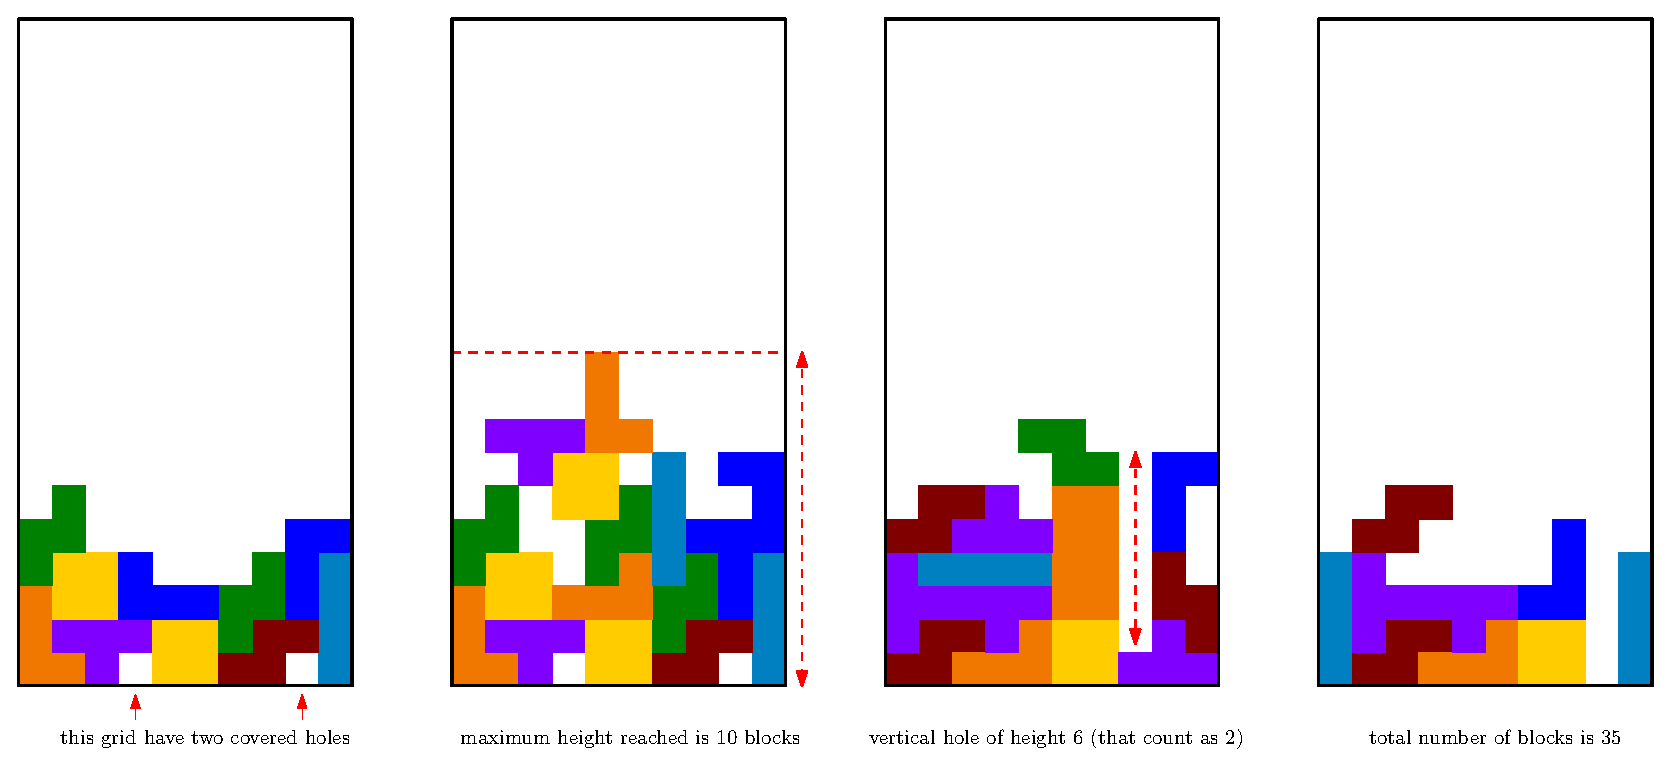
\includegraphics[width=\textwidth ]{images/grid_properties.eps}
    \caption{Grid's properties}
    \label{fig:tetris}
\end{figure}

This algorithm is critical since critical  aspects of the game may be cut-off by the horizon. Since we want to search \textit{as deeply as possible in a given time}, we could apply the \textit{iterative deepening search}, until the time's up, and then return the solution of the deepest completed search.\bigskip 

A better solution is called \textit{Quiescence search}, Instead of using a fixed search depth $d$, quiescence search dynamically adapts the depth to handle ''unquiet'' positions where the evaluation function's value is likely to fluctuate quickly—typically due to immediate, forcing moves like captures or checks.

For example, in Chess, if a piece exchange is underway, the search continues past the standard depth limit until a ''quiet'' state is reached, ensuring the final evaluated position is stable and doesn't miss an immediate, significant change in material or safety, thus leading to a much more accurate evaluation.

\subsection{Alpha-Beta Pruning}
There is a way to save time during the computation, we can cut-off some branches of the search for which we know at priori that will not lead to the solution. Consider the tree in figure \ref{fig:alphaPruning}.

\begin{figure}[h!]
    \centering
    \includegraphics[width=0.3\textwidth ]{images/alphapruning.png}
    \caption{Let's say $n>m$}
    \label{fig:alphaPruning}
\end{figure}

The left branch leads to a utility at least $n$, the right branch have one sub-branch with utility value $m<n$, so we can say for sure that the left tree will not provide values for the utility grater than $m$ (since it's the $Min$ turn), at this point we can discard the left branch and continue with the right one.\bigskip

We consider two additional variables $\alpha,\beta$ defined on each node during the search, such that:\begin{itemize}
    \item for each node $n$, $\alpha$ is the highest utility that search has already found for $Max$ on its path to $n$.\begin{itemize}
        \item In a $Min$ node, if one of the successors has a utility value less or equal than $\alpha$, we can stop considering $n$ and cutting it off  (pruning out its remaining successors).
    \end{itemize}
    \item We can consider a dual method for $Min$, for each node $n$, $\beta$ is the lowest utility that search has already found for $Min$ on its path to $n$.\begin{itemize}
        \item in a $Max$ node, if one of the successors has a utility value greater or equal than $\beta$, we can stop considering $n$ and cutting it off  (pruning out its remaining successors).
    \end{itemize}
\end{itemize}

%%%
 \begin{algorithm}
    \caption{AlphaBetaPruning}\label{alg:alphabetapruning}
    \begin{algorithmic}
    \Require $s$
    \State $v\leftarrow$MaxValue($s$,$-\infty$,$+\infty$)
    \State\Return an action $a\in $\texttt{Actions}($s$) yielding value $v$
    \end{algorithmic}
\end{algorithm}
 \begin{algorithm}
    \caption{MaxValue}\label{alg:ABMaxValue}
    \begin{algorithmic}
    \Require $s,\alpha,\beta$
    \If{TerminalTest($s$)}
    \State\Return $u(s)$
    \EndIf
    \State$v\leftarrow -\infty$
    \For{each $a\in $\texttt{Actions}($s$)}
    \State $v\leftarrow$ max($v$,MinValue(ChildState($s$,$a$)),$\alpha$,$\beta$)
    \State$\alpha\leftarrow\max(\alpha,v)$
    \State\textbf{if $v\ge\beta$ then return $v$}
    \EndFor 
    \State\Return $v$
    \end{algorithmic}
\end{algorithm}
  \begin{algorithm}
    \caption{MinValue}\label{alg:ABMaxValue}
    \begin{algorithmic}
    \Require $s,\alpha,\beta$
    \If{TerminalTest($s$)}
    \State\Return $u(s)$
    \EndIf
    \State$v\leftarrow +\infty$
    \For{each $a\in $\texttt{Actions}($s$)}
    \State $v\leftarrow$ min($v$,MaxValue(ChildState($s$,$a$)),$\alpha$,$\beta$)
    \State$\beta\leftarrow\min(\beta,v)$
    \State\textbf{if $v\le\alpha$ then return $v$}
    \EndFor 
    \State\Return $v$
    \end{algorithmic}
\end{algorithm}
%%%
\subsection{Monte-Carlo Tree Search}
The Alpha-Beta search have two issues\begin{itemize}
    \item it needs an accurate and fast evaluation function 
    \item it doesn't explore so much in problems with a large branching factor like \textit{Go}.
\end{itemize}
\begin{itemize}[leftmargin=*]
    \item \textbf{State Value Estimation:} The value of a state is estimated by calculating the average utility across multiple \textbf{playouts} (complete game simulations starting from that specific state).
    \item \textbf{Playout Policy:} During a playout, a policy is used to bias move selection toward ''good'' moves rather than purely random ones. For complex games like Go, these policies are often learned via \textbf{self-play} using neural networks.
    \item \textbf{Pure Monte Carlo Search:} This approach runs simulations from the current game state and tracks which possible moves yield the highest win percentage.
    \item \textbf{Selection Policy:} This policy optimizes computation by focusing on the most important branches of the game tree. Its primary function is to balance the trade-off between:
    \begin{itemize}
        \item \textbf{Exploration:} Searching less-visited parts of the tree to find potentially better moves.
        \item \textbf{Exploitation:} Deepening the search in branches already known to have high win rates.
    \end{itemize}
\end{itemize}
In the Monte Carlo Sampling we evaluate actions through sampling:\begin{itemize}
    \item Exploitation: play in the machine that returns the best reward.
    \item Exploration: play machines that have not been tried a lot yet.
\end{itemize}
The \textbf{UBC} (Upper Confidence Bound) is a formula that automatically balances
 exploration and exploitation to maximize total gains. The procedure of the search is described in the following steps:
\begin{enumerate}
    \item \textbf{Selection:} Starting at the root, traverse the tree by applying the \textit{selection policy} to choose successors until a leaf node that has not been fully expanded is reached.
    \item \textbf{Expansion:} Grow the search tree by generating a new child of the selected leaf node by applying a new action.
    \item \textbf{Simulation:} Perform a complete run of the game (a \textit{playout}) starting from the newly generated child node. Moves for both players are selected according to the \textit{playout policy} to obtain a final reward.
    \item \textbf{Back-propagation:} Use the result of the simulation to update the value estimates of all search tree nodes along the path back up to the root.
\end{enumerate}
Once the computational time or resources are exhausted, the algorithm chooses the ''best'' move based on the accumulated statistics and plays it.
We have to define a formula that balances exploration and exploitation, a formula  Inspired by Multi-Armed
 Bandit problems is the following\begin{equation}
    UBC1(n)=\frac{U(n)}{N(n)}+C\times\sqrt{\frac{\log N(PARENT(n))}{N(n)}}
 \end{equation}
where\begin{itemize}
    \item $U(n)$ is the total utility of all playouts that went through the node $n$
    \item $N(n)$ is the number of playouts through node $n$ 
    \item $PARENT(n)$ is the parent of $n$ in the tree. 
\end{itemize}
the left side of the sum represent the exploitation factor and the right side the exploration.
\begin{itemize}
    \item MTCS is chosen when branching factor becomes very high and the
     evaluation function is difficult.
     \item  MTCS is more robust than Alpha-Beta search (it is also possible to
 combine MCTS and evaluation functions).
 \item MTCS can be applied to unknown games. 
 \item  MTCS is a form of reinforcement learning.
\end{itemize}

\begin{algorithm}
    \caption{Monte-Carlo-Tree-Search}\label{alg:MTCS}
    \begin{algorithmic}
    \Require $state$
    \State $tree\leftarrow$Node($state$)
    \While{Is-Time-Remaining()}
    \State $leaf\leftarrow$Select($tree$)
    \State $child\leftarrow$Expand($leaf$)
    \State$result\leftarrow$Simulate($child$)
    \State Back-Propagate($result$,$child$)
    \EndWhile
    \State\Return the move in Actions($state$) whose node has highest number of playouts.
    \end{algorithmic}
\end{algorithm}














\chapter{Constraint Satisfaction Problems}
\begin{definition}
    A \textbf{CSP} (constraint satisfaction problem) is composed by a set of variables, each associated with it's domain, and a set of constraints over these variables, the goal is to find an assignment of variables so that every constraint is satisfied.
\end{definition}
In SuDoKu, the variables are the content of the cells, the domain of each cell is $\{1,2,\dots 9\}$, and the constraints are that, each number should appear only once in each row, column or block. Another CSP problem is the \textit{graph coloring} problem, where we should assign one of the $k$ possible color to each node, such that two adjacent nodes must have different colors (this problem is $\mathsf{NP}$-hard for $k=3$).
\section{Constraint Networks}
\begin{definition}
    A \textbf{Binary Constraint Network} is a tuple $\gamma=(V,D,C)$ where:
    \end{definition}\begin{itemize}
        \item $V=\{v_1,v_2\dots v_n\}$ is a finite set of variables. 
        \item $D=\{D_{v_1},D_{v_2}\dots D_{v_n}\}$ is a corresponding set of finite domains.
        \item $C$ is a set of binary relations that models the constraints. A relation is denoted $C_{uv}$ with $u,v$ variables in $V$. $$C_{uv}\subseteq D_u\times D_v$$If $C_{uv}\in C$ and $C_{xy}\in C$, then $\{u,v\}\ne \{x,y\}$ (no redundancy).
    \end{itemize}
    $C_{uv}$ defines the permissible combined assignments to $u$ and $v$. For example, let\begin{align}
        &u,v\in V\\
        &v'\in D_{v}\\ 
        &u' \in D_{u}\\ 
        & C_{uv}\subseteq D_{v}\times D_{u} \in C\\
    \end{align}
if $(v',u')\notin C_{uv}$ the assignment $v=v', u=u'$ violates the constraint, so $C_{uv}$ contains the permissible combined assignments for two variables. Let's see an example, we consider the map of australia show in figure \ref{fig:australia}. We want to colorate each state with one of 3 possible colors, without having two adjacent state with the same color.\bigskip

\begin{figure}[h!]
    \centering
    \includegraphics[width=0.5\textwidth ]{images/australia.png}
    \caption{Coloring Australia}
    \label{fig:australia}
\end{figure}

\noindent The variables are the states 
$$ V=\{WA,NT,SA,Q,NSW,V,T\}$$
The domain for each variable $v\in V$ is $D_v=\{red,green,blue\}$.
If all the variables have the same domain \begin{equation}
    \forall v\ne u, D_v=D_u
\end{equation}
as a notation abuse we say that the domain of the problem is $D=\{red,green,blue\}$.
For each adjacent couple of states $u,v$, there is a constraint
$$C_{uv}=\{(d,d')\in D\times D \ : \ d\ne d'\}.$$
Constraint Networks can be extended\begin{itemize}
    \item the domains $D_v$ may be infinite or uncountable, like $D_v=\R$.
    \item the constraints may have an arity higher than 2, with relations over $k>2$ variables, like in CNF satisfiability.
\end{itemize}
A constraint may be \textbf{unary}: $C_v\subseteq D_v$, in this case the domain of a single variable is restricted, equivalently to setting $D_v=C_v$.\bigskip 

There exists CSP solvers, generic algorithms that find assignment for constraints problem, by taking in input a constraint network as the generic language to describe the problem. The core exercise in this context is to model a problem with a constraint network.
\begin{definition}
    Let $\gamma=(V,D,C)$ to be a constraint network, a \textbf{partial assignment} is a function $$a:V'\rightarrow \bigcup_{v\in V}D_v$$ where \begin{itemize}
        \item $V'\subseteq V$
        \item $a(v)\in D_v$ for all $v\in V'$
    \end{itemize}
if $V'=V$ is a \textbf{total assignment} (or just assignment). A partial assignment assigns a value to some variables from their
respective domains. A total assignment is defined on all variables.
\end{definition}
\begin{definition}
    Let $\gamma=(V,D,C)$ to be a constraint network and let $a$ to be a partial assignment, we say that $a$ is \textbf{inconsistent} if there exists variables $u,v\in V$ such that
\end{definition}
\begin{itemize}
        \item $a$ is defined on $u$ and $v$
        \item $C_{uv}\in C$
        \item $(a(u),a(v))\notin C_{uv}$.
    \end{itemize}
If a partial assignment is not inconsistent, is \textbf{consistent}. An assignment $a$ is a \textbf{solution} if it's total and consistent. A constraint network $\gamma$ is \textbf{solvable} if there exists a solution $a$, otherwise is \textbf{unsolvable}.\begin{center}
    \includegraphics[width=0.8\textwidth ]{images/australia2.png}
\end{center}
\begin{definition}
    Let $\gamma=(V,D,C)$ to be a constraint network, and let $a$ to be a partial assignment. $a$ can be \textbf{extended} to a solution if there exists a solution $a'$ that agrees with $a$ on the variables where $a$ is defined.
\end{definition}
\begin{itemize}
    \item the domain of $a$ is $V'\subset V$
    \item for each $v\in V'$, we have that $a(v)=a'(v)$.
\end{itemize}
\begin{proposition}
    if $a$ can be extended to a solution, then it's consistent (the opposite doesn't necessary holds).
\end{proposition}
Given a constraint network $\gamma=(V,D,C)$, if $n=|V|$ and $\forall D_v\in D$, $|D_v|=k$, the number of total assignments is $k^n$. There are at most $n^2$ constraints, each constraint have size at most $k^2$, the number of assignments is \textit{exponentially bigger} than the size of $\gamma$.\begin{theorem}
    The problem to decide if a constraint network $\gamma=(V,D,C)$, is solvable is  $\mathsf{NP}$-complete.
\end{theorem}
\section{Naive Backtracking}
The following algorithm is simple and used to find a solution for a constraint network. The method is recursive, the initial assignment $a$ to start the algorithm is the empty assignment.
 \begin{algorithm}
    \caption{NaiveBacktracking}\label{alg:NaiveBacktracking}
    \begin{algorithmic}
    \Require $\gamma=(V,D,C),a$
    \If{$a$ is inconsistent} \State\Return inconsistent\EndIf
    \If{$a$ is a total assignment} \State\Return $a$\EndIf
    \State let $V'$ to be the domain of $a$
    \State select \color{blue} some  \color{black} $v\in V-V'$ \greenText{/*select a variable for which $a$ is not defined*/}
    \For{ each $d\in D_v$ in \color{blue} some order \color{black}}
    \State $a'=a\cup \{v=d\}$
    \State $a''=$NaiveBacktracking($\gamma$,$a'$)
    \If{$a''$ is consistent} \State\Return $a''$\EndIf
    \EndFor
    \State\Return inconsistent
    \end{algorithmic}
\end{algorithm}
With \textit{Backtracking}, we mean the action of recursively instantiate variables one-by-one, backing up out
of a search branch if the current partial assignment is already inconsistent.
Note that in the algorithm \ref{alg:NaiveBacktracking} we are iterating the possible values in $D_v$ in a specific \color{blue} order \color{black} that is not described yet, and is not described which variable are we picking at each recursion step.\bigskip 

\noindent The Naive Backtracking algorithm is\begin{itemize}
    \item simple to implement 
    \item much more efficient than enumerating all possible assignment
    \item complete, if there is a solution, backtracking
will find it.
\end{itemize}
This algorithm can't predict if an assignment $a$ can't be extended to a solution unless $a$ is already inconsistent.
\subsection{About the Order}
The ordering in the for loop of algorithm \ref{alg:NaiveBacktracking} can  influences the search space size. If no solution exists below current node, the order doesn't matter, the algorithm will search the whole sub-tree anyway, otherwise, if a solution does exist below current node, by choosing the ''correct'' value, then no backtracking is needed.\bigskip 

A common strategy is to consider the variable ''most constrained'' (the variable with the greatest number of assignments that make $a$ inconsistent), at each recursion step, we pick the variable $v$ that minimize the size of the set\begin{equation}
    \{d\in D_v \ : \ a\cup\{v=d\} \text{ is consistent }\}
\end{equation}
by choosing a most constrained variable $v$ first, we reduce the
branching factor (number of sub-trees generated for $v$) and thus reduce
the size of our search tree.\bigskip 

Another common heuristic is to choose the variable that is the ''most constraining'' (the most frequent variable in constraints), we choose $v$ that maximize the size of the set\begin{equation}
    \{u\in V \ : \ a(u)\text{ is undefined }\land \left(C_{uv}\in C \lor C_{vu}\in C\right) \}
\end{equation}
by choosing a most constraining variable first, we detect
inconsistencies earlier on and thus reduce the size of our search tree.\bigskip 

For the order of the value in the for loop, we can choose the least constraining value first, for a variable $v$, we choose the value $d\in D_v$ that minimize the size of the set\begin{equation}
    \{d' \ : \ d'\in D_u\land a(u)\text{ is undefined }\land C_{uv}\in C\land (d',d)\notin C_{uv}\}
\end{equation}
by choosing a least constraining value first, we increase the chances
to not rule out the solutions below the current node. 
\section{Inference}
Given a constraint network, we would like to obtain an equivalent network with more constraint, without losing any feasible solution, in such case, we are giving a tighter description of the problem, and we obtain a network with a smaller number of
consistent partial assignments. Already known constraints may implies additional (unary or binary) constraints.\begin{definition}
    Let $\gamma=(V,D,C)$ and $\gamma'=(V,D',C')$ to be two constraint networks, sharing the same set of variables. We say that $\gamma$ are \textbf{equivalent} to $\gamma'$, and we denote $$ \gamma\equiv\gamma' $$
    if every solution (assignment of variables) of $\gamma$ is a solution of $\gamma'$ and vice versa.
\end{definition}
\begin{definition}
    Let $\gamma=(V,D,C)$ and $\gamma'=(V,D',C')$ to be two constraint networks, sharing the same set of variables. We say that $\gamma'$ is \textbf{tighter} than $\gamma$ and we denote $$ \gamma'\sqsubseteq \gamma $$
    if
\begin{itemize}
    \item $\forall v\in V, \ \ D'_v\subseteq D_v$
    \item $\forall u,v \text{ such that }u\ne v$ either $C_{uv}\notin C$ or $C'_{uv}\subseteq C_{uv}$.
\end{itemize}\end{definition}
If at least one of these inclusions is strict, we say that  $\gamma'$ is \textbf{strictly tighter} than $\gamma$: $$ \gamma'\sqsubset \gamma. $$\begin{theorem}
    Let $\gamma$ and $\gamma'$ to be two constraint networks, if\begin{itemize}
        \item $\gamma'\equiv\gamma$
        \item $\gamma'\sqsubset\gamma$
    \end{itemize}
    then $\gamma'$ has the same solutions as $\gamma$ but fewer consistent partial
assignments than $\gamma$. In such case, $\gamma'$ is a \textbf{better encoding} of the problem.
\end{theorem}
We define \textit{inference} the procedure to derive a tighter equivalent network. We want to use it to define an algorithm that finds a solution for a constraint network. We will incorporate inference in the  backtracking algorithm, at every recursive call, a complex inference procedure leads to\begin{itemize}
    \item a smaller  number of search nodes 
    \item larger runtime needed at each node
\end{itemize} 
We encode partial assignments as unary constraints\begin{itemize}
    \item if $a(v)=d$
    \item we set the constraint $D_v=\{d\}$
\end{itemize}

\begin{algorithm}
    \caption{BacktrackingWithInference}\label{alg:BacktrackingWithInference}
    \begin{algorithmic}
    \Require $\gamma=(V,D,C),a$
    \If{$a$ is inconsistent} \State\Return inconsistent\EndIf
    \If{$a$ is a total assignment} \State\Return $a$\EndIf
    \State $\gamma'=$ copy of $\gamma$
    \State \color{orange}$\gamma'=$ Inference$(\gamma')$\color{black}
    \State\textbf{If} $\exists v \ : \ D'_v=\emptyset$ \textbf{ then return } inconsistent
    \State let $V'$ to be the domain of $a$
    \State select \color{blue} some  \color{black} $v\in V-V'$ (select a variable for which $a$ is not defined)
    \For{ each $d\in D'_v$ in \color{blue} some order \color{black}}
    \State $a'=a\cup \{v=d\}$
    \State $D'_v=\{d\}$
    \State $a''=$NaiveBacktracking($\gamma'$,$a'$)
    \If{$a''$ is not inconsistent} \State\Return $a''$\EndIf
    \EndFor
    \State\Return inconsistent
    \end{algorithmic}
\end{algorithm}
With the function \color{orange}Inference \color{black} we denote any procedure deriving a tighter equivalent network. One simple inference procedure called \textit{forward checking} is described in algorithm \ref{alg:FWCH}.\bigskip 

\begin{algorithm}
    \caption{Forward Checking}\label{alg:FWCH}
    \begin{algorithmic}
    \Require $\gamma,a$
    \For{ each $v$ where $a(v)=d'$ is defined }
    \For{ each $u$ where $a(u)$ is undefined and $C_{uv}\in C$}
    \State $D'_u=\{d \ | \ d\in D_u, (d,d')\in C_{uv}\}$
    \State $D_u\leftarrow D'_u$ \greenText{/*We update the domain of $u$*/}
    \EndFor 
    \EndFor 
     \State\Return $\gamma$
    \end{algorithmic}
\end{algorithm}

The forward checking algorithm tightens the constraints without ruling out any solutions, it guarantees to deliver an equivalent network. The computation can be done incrementally, instead of performing the first loop, we may run only the second loop every time a new assignment $a(v)=d'$ is added.\begin{itemize}
    \item The forward checking procedure is cheap and useful 
    \item In rare situations is not a good idea to use it, there are stronger inference methods, but in many cases, forward checking is the best choice.
\end{itemize}

\subsection{Arc Consistency for Stronger Inference}
We now describe a property between two variables that can be used to describe a stronger inference method than forward checking.\begin{definition}
    Let $\gamma=(V,D,C)$ to be a constraint network, a variable $u\in V$ is \textbf{arc consistent} to another variable $v\in V$ if \begin{itemize}
            \item either $C_{uv}\notin  C$ 
            \item or for every $d\in D_u$ there exists $d'\in D_v$ such that $(d,d')\in C_{uv}$.
    \end{itemize}
\end{definition}
When two variables in a constraint network are arc consistent, it means that the domain  of each variable contains at least one value that is compatible with at least one value in the domain of the other variable, according to the constraint between them.

As an example, let's say the variable $v$ describes the color of your shirt, that can be red, blue, yellow or green, and the variable $u$ define the color of your pants, that can be black, white, gray or brown. The constraint is that the shirt and the pants cannot be the same color, the variable $v$ is  arc consistent to $u$ because for every shirt color you can find a pants color and vice versa.\begin{quote}
    \textbf{Note}: Arc consistency is a non commutative relation, if $v$ is  arc consistent to $u$, it's not implied directly that $u$ is  arc consistent to $v$.
\end{quote}
\begin{definition}
    Let $\gamma=(V,D,C)$ to be a constraint network, if every variable $u\in V$ is arc consistent relative to every other variable $v\in V$, then we say that the network $\gamma$ is \textbf{arc consistent}.
\end{definition}
We can define an inference procedure that aims to make the network $\gamma$ arc consistent, by removing variable domain values. Let's say that AC($\gamma$) is a procedure that makes $\gamma$ arc consistent, in such case:\begin{itemize}
    \item is guaranteed that AC($\gamma$) returns an equivalent network.
    \item AC($\gamma$) is more powerful (more general) the forward checking, in details:\begin{equation}
        \text{AC}(\gamma)\sqsubseteq \text{ForwardChecking}(\gamma)
    \end{equation}
\end{itemize}
We define the following subroutine:

\begin{algorithm}
    \caption{Revise}\label{alg:revise}
    \begin{algorithmic}
    \Require $\gamma,u\in V,v\in V$
    \For{ each $d\in D_u$}
    \If{$\lnot\exists d'\in D_v$ such that $(d,d')\in C_{uv}$}
    \State $D_u=D_u\backslash\{d\}$
    \EndIf
    \EndFor 
     \State\Return $\gamma$
    \end{algorithmic}
\end{algorithm}

We apply pairwise Revisions in algorithm \ref{alg:AC1} and define the first version of the inference procedure that makes a constraint network $\gamma$ arc consistent.\bigskip

\begin{algorithm}
    \caption{AC\_1}\label{alg:AC1}
    \begin{algorithmic}
    \Require $\gamma$
    \State changes = False
    \While{changes = False }
    \For{ each $C_{uv}\in C$}
    \State\textbf{If } $D_u$ after applying Revise($\gamma,u,v$) is reduced \textbf{ then } changes = True
    \State\textbf{If } $D_v$ after applying Revise($\gamma,v,u$) is reduced \textbf{ then } changes = True
    \EndFor
    \EndWhile
    \end{algorithmic}
\end{algorithm}

It's not hard to show that this enforce arc consistency. If there are $n$ variables, $m$ constraints and $k$ is the cardinality of the biggest domain, then the time complexity is $O(mk^2\cdot nk)$, this algorithm performs redundant computation since $u$ and $v$ are revised even if their domains
haven't changed since the last time.\bigskip 

\noindent There is another version of the arc consistency procedure, described in algorithm \ref{alg:AC3}. At any moment during the while loop, if $(u,v)\notin M$ then $u$ is arc consistent to $v$.

\begin{algorithm}
    \caption{AC\_3}\label{alg:AC3}
    \begin{algorithmic}
    \Require $\gamma$
    \State $M=\emptyset$
     \For{ each $C_{uv}\in C$}
     \State $M=M\cup\{(u,v),(v,u)\}$
     \EndFor
      \While{$M\ne\emptyset$ }
      \State remove a random single element $(u,v)$ from $M$
      \State Revise($\gamma,u,v$)
      \If{ $D_u$ has changed in the call Revise}
      \For{ each $C_{wu}\in C$ where $w\ne v$}
      \State $M=M\cup\{(w,u)\}$
       \EndFor
      \EndIf 
      \EndWhile
    \end{algorithmic}
\end{algorithm}

In the algorithm, we check the constraints where $w\ne v$ because $v$ is the reason why $D_u$ just changed, if $v$ was arc consistent to $u$ before, that continues to hold, the values just removed from $D_u$ did not match any values from $D_v$ anyway.
\begin{theorem}
    Let $\gamma$ to be a constraint network with $m$ constraint and maximal domain size $k$. The algorithm AC3 showed in \ref{alg:AC3} have a time complexity in $O(mk^3)$.
\end{theorem}
\textit{Proof}: Each Revise call takes $O(k^2)$, it is sufficient to prove that at most $O(mk)$ calls to revise are made. 
The number of calls to Revise is the number of iterations of the
while-loop, which is at most the number of insertions into $M$. \begin{itemize}
    \item Consider
    any constraint $C_{uv}$
    \item two variables pairs corresponding to the constraint $C_{uv}$ are inserted into $M$ in the first for loop
    \item then
beforehand the domain of either $u $ or $v$ was reduced, which happens at
most $2k$ times 
\item thus we have $O(k)$ insertions per constraint, and $O(mk)$ insertions overall.\hfill$\blacksquare$
\end{itemize}

\section{Decomposition}
If $\gamma$ is a network with $n$ variables and maximal domain size $k$, we may search a feasible assignment by checking among all the possible ones, this will require to check $O(k^n)$ assignments in the worst case. We saw how the inference help to shrink the search space, another useful methods is called \textit{decomposition}.\begin{quote}
    \textbf{decomposition}: exploit the structure of a network to decompose it into smaller (and easier to solve) independent networks.
\end{quote}
\begin{definition}
    Given a constraint network $\gamma=(V,D,C)$, the \textbf{constraint graph} of $\gamma$ is the undirected graph, where the vertices are the variables $V$ and there are an edge $(u,v)$ if $C_{uv}\in C $.
\end{definition}
For example, the graph for the ''coloring Australia'' problem shown in figure \ref{fig:australia} is the following:\begin{center}
    \includegraphics[width=0.4\textwidth ]{images/australia_graph.png}
\end{center}
Note how this graph is composed by two connected sub-graph, since the variable $T$ (Tasmania) is disconnected from the other variables. The idea is to separate a network in function of his connected sub-graphs.  
\begin{theorem}
    Let $\gamma=(V,D,C)$ to be a constraint network. Let $G$ to be the constraint graph, we denote $\mathcal V(G)$ the vertices of $G$ and $\mathcal E(G)$ the edges of $G$, we know that $\mathcal V(G)=V $. We consider a partition of $\mathcal V(G)$\begin{equation}
        \mathcal V(G)=\bigcup_i V_i
    \end{equation}
    such that each $V_i$ is connected and $$\begin{cases}
        v\in V_i\\ 
        u\in V_j\\ 
        V_i\ne V_j
    \end{cases}\implies\begin{matrix}
     (u,v)\notin \mathcal E(G)\\ 
      (v,u)\notin \mathcal E(G)
    \end{matrix} \implies C_{uv}\notin C$$
    so the components of the partition are disconnected from each other. Let $a_i$ to be a feasible assignment (solution) for the variables $V_i$, then \begin{equation}
        a=\cup_i a_i 
    \end{equation}
    is a solution to $\gamma$.
\end{theorem}
The theorem states that if two parts of $\gamma$ are not connected (in term of his constraint graph), then they are independent and we can find separately a solution for each connected component.\bigskip 

\begin{theorem}
    Let $\gamma=(V,D,C)$ to be a constraint network with $n$ variables and maximal domain size $k$. Let $G$ to be the constraint graph, if $G$ is acyclic, we can find a solution for $\gamma$ (or prove that $\gamma$ is inconsistent) with a time complexity of $O(nk^2)$.
\end{theorem}
The procedure is the following (assuming that a constraint network is connected, if not, we can apply the procedure to each connected component).\begin{enumerate}
    \item We consider the constraint graph of $\gamma$, denoted $G$. We choose an arbitrary node $v\in \mathcal V(G)=V$, and we consider the BFS spanning tree $G'$ starting from $v$. 
    \item $G'$ is a directed graph, we consider a topological ordering $v_1\dots, v_n$ of the variables.
    \item we iterate through the variables $v_i$ in the opposite order respect to the topological ordering: for each $i=n-1,n-2,\dots, 3,2$ (except for $v_1$)\begin{enumerate}
        \item we perform the procedure Revise($\gamma$, parent($v_i$), $v_i$)
        \item if $D_{\text{parent($v_i$)}}\ne \emptyset$, return inconsistent
    \end{enumerate}
    at this point,  every variable is arc consistent relative to its children
    \item We perform the algorithm \ref{alg:BacktrackingWithInference} using the variable order $v_1,v_2\dots , v_n$.
\end{enumerate}
We call this procedure $AcyclicCG(\gamma)$.
\subsection{Cutsets}
\begin{definition}
    Let $\gamma=(V,D,C)$ to be a constraint network. Let $G$ to be the constraint graph, a \textbf{cutset} $V_0\subseteq V$ is a set such that, the graph $G'$ where $\mathcal V(G')=V\backslash V_0$ is acyclic.
\end{definition}
A cutset is a subset of variables removing which renders the constraint
graph acyclic. The graph of the ''coloring Australia'' problem is \textit{almost acyclic} since, removing $SA$ will make the graph a tree.\begin{center}
    \includegraphics[width=0.6\textwidth ]{images/australia_graph2.png}
\end{center}
The following procedure use cutsets to find a solution for $\gamma$.

\begin{algorithm}
    \caption{CutsetConditioning}\label{alg:CutsetConditioning}
    \begin{algorithmic}
    \Require $\gamma,V_0,a$
    \State $\gamma'=$ a copy of $\gamma$
    \State $\gamma'=$ Forward Checking($\gamma'$,a)
    \State\textbf{if} $\exists v$ with $D'_v=\emptyset$ \textbf{then return} inconsistent 
    \If{ $\exists v\in V_0$ such that $a(v)$ is undefined}
    \State select such \blueText{$v$} \greenText{/*used after this if-else block*/}
    \Else  
    \State $a'=AcyclicCG(\gamma')$
    \State\textbf{if} $a'\ne$inconsistent \textbf{then return} $a\cup a'$ 
    \State\textbf{else return} inconsistent 
    \EndIf 
    \State we consider the selected \blueText{$v$}
    \For{each $d\in$ copy of $D'_v$ in some order}
    \State $a'=a\cup\{v=d\}$
    \State $D'_v=\{d\}$
    \State $a''=$CutsetConditioning($\gamma',V_0,a'$)
    \State\textbf{if} $a''\ne$inconsistent \textbf{then return} $a''$.  
    \EndFor 
    \State\Return inconsistent 
    \end{algorithmic}
\end{algorithm}

\noindent\textbf{Algorithm explanation}:
\begin{itemize}[label=\textbullet]
    \item \textbf{Initialization and Propagation}: 
    The algorithm begins by creating a local copy of the network ($\gamma'$) and applying \textbf{Forward Checking}. This ensures that the current assignments ($a$) are consistent with the remaining domains. If any domain $D'_v$ becomes empty, the current branch is deemed \textit{inconsistent}.

    \item \textbf{Cycle Cutset Processing ($V_0$)}:
    The algorithm prioritizes variables belonging to the cutset $V_0$.
    \begin{itemize}
        \item If there are unassigned variables in $V_0$, the algorithm selects one ($v$) to branch on.
        \item It enters a recursive search where it tries every possible value $d$ from the domain $D'_v$. 
        \item By assigning values to all variables in $V_0$, the algorithm effectively ''breaks'' the cycles in the constraint graph.
    \end{itemize}

    \item \textbf{Base Case: Solving the Acyclic Subproblem}:
    Once all variables in the cutset $V_0$ are assigned, the remaining network is \textbf{acyclic}. 
    \begin{itemize}
        \item The algorithm calls \texttt{AcyclicCG($\gamma'$)}.
        \item Because tree-structured CSPs can be solved in linear time (using arc consistency algorithms like AC-3 or specialized directional consistency), this step is highly efficient.
        \item If the acyclic solver finds a valid assignment $a'$, it is merged with the cutset assignments $a$ and returned as the solution.
    \end{itemize}

    \item \textbf{Backtracking Search}:
    If the recursive call \texttt{CutsetConditioning} or the \texttt{AcyclicCG} call returns \textit{inconsistent}, the algorithm backtracks, picks the next value in the domain of $v$, and tries again.

    \item \textbf{Termination}:
    The algorithm returns a complete, consistent assignment $a \cup a'$ if one exists; otherwise, after exhausting all possibilities for the cutset variables, it returns \textit{inconsistent}.
\end{itemize}

The forward checking operation is required to ensure that $a\cup a'$ is consistent in $\gamma$, the runtime is exponential in $V_0$. It is true that finding an optimal cutset for a graph is $\mathsf{NP}$-hard, but practical approximated procedures exists.



\chapter{Logic and Knowledge Representation}
\section{Propositional Logic}
This chapter presents a brief summary of propositional logic. Let $\Sigma$ to be a set of boolean variables, also called \textit{Atoms}, the definition of a formula over the variables $\Sigma$ is recursive.\begin{definition}
    Let $\Sigma$ to be a set of atoms, then\begin{enumerate}
        \item $\top$ (True) and  $\bot$ (False) are $\Sigma$-formulas.
        \item Each atom $P\in \Sigma$ is a $\Sigma$-formula. 
        \item If $\varphi$ is a formula\footnote{
            We abbreviate ''$\Sigma$-formula'' with ''formula'' leaving it implicit that the formula is on the set of variables defined in the context.
        }, then $\lnot \varphi$ is a formula.
    \end{enumerate}
\end{definition}
If $\varphi$ and $\psi$ are formulas then:\begin{enumerate}
    \item $\varphi\land \psi$ is a formula (\textit{conjunction})
    \item $\varphi\lor \psi$ is a formula (\textit{disjunction})
    \item $\varphi\rightarrow \psi$ is a formula (\textit{implication})
    \item $\varphi\leftrightarrow \psi$ is a formula (\textit{equivalence})
\end{enumerate}
We recall that \begin{align}
    &\varphi\rightarrow \psi\equiv \lnot \varphi \lor \psi \\ 
    &\varphi\leftrightarrow \psi \equiv (\varphi \land \psi)\lor(\lnot\varphi \land \lnot\psi)
\end{align}
\begin{definition}
    An \textbf{interpretation} $I$ over $\Sigma$ is an assignment $I:\Sigma\rightarrow \{0,1\}$.
\end{definition}
We say that $I$ \textbf{satisfy} a formula $\varphi$, and we write $I\models \varphi$ if the assignment makes the formula true. We can also say that $I$ is a \textbf{model} of $\varphi$ and the set of all the models of $\varphi$ (all the assignments that satisfies $\varphi$) is denoted $M(\varphi)$.

\textbf{Example}:\begin{equation}
    \varphi = (P\lor Q)\iff (R\lor S) 
\end{equation}
the interpretation \begin{equation}
    I=\begin{cases}
        P=1\\ 
        Q=0\\ 
        R=1\\ 
        S=1
    \end{cases}
\end{equation}
is a model since $I\models \varphi$:\begin{equation}
    (P\lor Q)\leftrightarrow (R\lor S)  \implies (1\lor 0)\leftrightarrow (1 \lor 1) \implies 1 \leftrightarrow 1 \implies \top
\end{equation}
Notation-wise, 0 and $\bot$ are interchangeable, like 1 and $\top$. A set of formulas $KB$ is called \textbf{Knowledge Base} and an interpretation $I$ models $KB$ if, for all $\varphi\in KB$ we have that $I\models \varphi$. We also say that $I$ is a model of $KB$.
\begin{definition}
    Let $\varphi$ to be a formula:\begin{itemize}
        \item $\varphi$ is \textbf{satisfiable} if $\exists I$ such that $I\models \varphi$ 
        \item $\varphi$ is \textbf{unsatisfiable} if is not satisfiable.
        \item $\varphi$ is \textbf{falsifiable} if there exists $I$ that doesn't satisfy $\varphi$.
        \item $\varphi$ is a \textbf{tautology} if $\forall I$, $I\models \varphi$ (it's not falsifiable).
    \end{itemize}
\end{definition}
\begin{definition}
    Two formulas $\varphi$ and $\psi$ are \textbf{equivalent}$$\varphi\equiv \psi $$ if $M(\varphi)=M(\psi)$ ($I$ models $\varphi$ if and only if models also $\psi$).
\end{definition}
\begin{definition}
    Let $\Sigma$ to be a set of atoms, a knowledge base $KB$ over $\Sigma$ \textbf{entails} a formula $\varphi$ $$KB\models \varphi $$
    if, all the models $I$ of $KB$, are models of $\varphi$. 
    $$ M(\bigwedge_{\psi\in KB}\psi)\subseteq M(\varphi)$$
\end{definition}
We say that the formula $\varphi$ follows from $KB$, and would be redundant to include $\varphi$ in $KB$. It's also important to derive new logic formula from a given knowledge base.
\begin{theorem}
    $KB\models \varphi$ if and only if $KB\cup\{\lnot \varphi\}$ is unsatisfiable.
\end{theorem}
\textit{Proof $\implies$}: Let $KB\models \varphi$ for any $I\models KB$ we have $I\models \varphi$ so $I\not\models \lnot \varphi$.

\noindent\textit{Proof $\impliedby$}: If $KB\cup\{\lnot \varphi\}$ is unsatisfiable then for any $I$ such that $I\models KB$ we have $I\not\models\lnot\varphi$ hence $I\models\varphi$.\bigskip 

Given a formula with $n$ variables, the number of possible assignment is $2^n$, so it's hard to test the satisfiability of a formula by testing all the  interpretations.\begin{definition}
    A formula is in \textbf{conjunctive normal form (CNF)} if is a conjunction of disjunction of literals.\footnote{A literal is an atom $P$ or the negation of an atom $\lnot P$.
    If $l=\lnot P$ where $P$ is an atom, the literal $\lnot l$ is equal to $P$.
    }.\begin{equation}
        \bigwedge_i\left(\bigvee_j l_{i,j}\right)
    \end{equation}
\end{definition}
\begin{definition}
    A formula is in \textbf{disjunctive normal form (DNF)} if is a disjunction of conjunction of literals.\begin{equation}
        \bigvee_i\left(\bigwedge_j l_{i,j}\right)
    \end{equation}
\end{definition}
It is important to know that \textbf{every formula} can be expressed in CNF or DNF, or, for each formula $\varphi$, there exists an equivalent formula $\psi$ that is a CNF or a DNF. It is possible to construct the equivalent CNF (or DNF) from $\varphi$ by exploiting the equivalences such as\begin{itemize}
    \item $\varphi \rightarrow \psi\equiv \lnot\varphi\lor\psi$
    \item $\lnot(\varphi\lor \psi)\equiv \lnot \varphi\land \lnot \psi$
    \item and so on...
\end{itemize}
$$\begin{aligned}
& ((P \lor H) \land \neg H) \to P && \text{Eliminate } "\to" \\
& \neg ((P \lor H) \land \neg H) \lor P && \text{Move } "\neg" \text{ inwards} \\
& (\neg (P \lor H) \lor H) \lor P && \text{Move } "\neg" \text{ inwards} \\
& ((\neg P \land \neg H) \lor H) \lor P && \text{Distribute } "\lor" \text{ over } "\land" \\
& ((\neg P \lor H) \land (\neg H \lor H)) \lor P && \text{Distribute } "\lor" \text{ over } "\land" \\
& (\neg P \lor H \lor P) \land (\neg H \lor H \lor P)
\end{aligned}$$
\subsection{Resolution}
We can construct a simple algorithm that, given a CNF formula $\psi$, tests if is satisfiable or not, by trying to derive from $\psi$ new formulas: If it finds a derived  formula $\psi$ that is unsatisfiable then $\psi$ is unsatisfiable.\bigskip 

We use a method called \textit{Calculus} that, given a single \textit{rule} (we will define a rule later), allows us to derive new formulas from a given one. If $\varphi$ is derived from $\psi$, we write $$\psi\vdash \varphi .$$
\begin{definition}
    A clause $C$ is a disjunction of literals, like:\begin{equation}
        \lnot P \lor Q \lor R \lor \lnot Q
    \end{equation}
    To shrink the notation, we identify $C$ with the set of the literals included:\begin{equation}
        P\lor \lnot Q \text{ became }C=\{P,\lnot Q\}
    \end{equation}
\end{definition}
Since a CNF is a conjunction of disjunction we can identify each CNF with a set of clauses, usually denoted $\Delta$. For example, the CNF\begin{equation}
    \Delta = \{\{P,\lnot Q\},\{R, Q\}\}
\end{equation}
is \begin{equation}
    (P\lor \lnot Q)\land (R\lor Q)
\end{equation}
We denote the empty clause $\square$. An interpretation $I$ satisfies a single clause $C$ $$I\models C$$ if there exists a literal $l\in C$ such that $I\models l$. $I$ satisfies $\Delta$ 
$$ I\models \Delta$$ 
if, for all $C\in \Delta$ we have that $I\models C$.
\begin{definition}
    A \textbf{inference rule} is a rule that derive a new formula from a given one, the \textbf{resolution rule} is the following:\begin{equation}
        \frac{C_1\dot\cup \{l\},C_2\dot\cup\{\lnot l\}}{C_1\cup C_2}
    \end{equation}
\end{definition}
You may wonder what this formula means and how it is applied, the symbol $\dot\cup$ identify a disjoint union, so $C_1\dot\cup \{l\}$ is a union and is implied that $l\notin C_1$. $l$ is a literal. The formula is written as a fraction:\begin{itemize}
    \item the term over the fraction line represents the clauses that we already have in our CNF 
    \item the term under the fraction line represents a new formula that we derive 
\end{itemize}
In practice, if we have two clauses $C'_1=C_1\dot\cup\{l\}$ and $C'_2=C_2\dot\cup\{\lnot l\}$ in $\Delta$, we can derive a disjunction (i.e. a new clause) $\phi = C_1\cup C_2$. The two starting clauses $C'_1$ and $C'_2$ are called parent clauses.\begin{quote}
    if you have two clauses where the same literal appears, but in one it is affirmative ($l$) and in the other it is negated ($\bar{l}$), you can ''add them'' by eliminating $l$ and $\bar{l}$ and merging everything else.
\end{quote}
For example, if you have $\{P,\lnot R\}$ and $\{R,Q\}$, you can resolve them and find a new formula $\{P,Q\}$.
\begin{theorem}\label{Teo:Soundness}
    The \textbf{soundness theorem} affirms that, if $\Delta\vdash D$ (the formula $D$ can be derived by some clause in $\Delta$ with the resolution rule) then $\Delta\models D$ (the CNF $\Delta$ entails $D$).
\end{theorem}
In practice, a resolution rule is \textbf{sound} if it derives formulas that are logically consistent with the parent clauses.\bigskip

In the definition of \textit{entailment}, is a knowledge base that ''entails'' a formula, and not a formula that ''entails'' another formula, but a knowledge base $KB$ is equivalent to a CNF by putting in conjunction all the formulas in $KB$.\bigskip 

The resolution algorithm takes as an input a knowledge base $KB$ and a formula $\phi$ and guess if $KB\models \phi$ by the following steps:\begin{enumerate}
    \item transform $KB$ in a CNF 
    \item write the CNF as a set of clauses $\Delta$, by adding to $\Delta$ also the clause $\{\lnot \phi\}$
    \item apply the resolution rule on $\Delta$ until it's derived the empty clause $\square$.
\end{enumerate}
\begin{center}
    \includegraphics[width=0.8\textwidth ]{images/resolution.png}
\end{center}
It is important to notice that $\Delta\models \varphi$ doesn't implies that $\Delta\vdash\varphi$, but, by the contradiction theorem, if we run the resolution on $KB\cup\{\lnot \varphi\}$ and we derive the empty clause $\square$ ($KB\cup\{\lnot \varphi\}$ is unsatisfiable) then $KB\models \varphi$.\begin{theorem}
    A CNF $\Delta$ is unsatisfiable if and only if $\Delta\vdash\square$.
\end{theorem}
\subsection{The DPLL procedure}
The SAT problem is to decide whenever a given propositional formula $\varphi$ is satisfiable or not, as we well know, this is the most classic example of a problem $\mathsf{NP}$-complete. The SAT problem is a ''subset'' of the constraint satisfaction problem:\begin{itemize}
    \item SAT can be viewed as a CSP problem in which all variable domains
 are Boolean, and the constraints have unbounded arity.
\end{itemize}
Every CSP problem can be encoded as a SAT problem:\begin{itemize}
    \item Given any constraint network $\gamma$, we can in low-order polynomial time
 construct a CNF formula $\varphi(\gamma)$ that is satisfiable if and only if $\gamma$ is solvable.
\end{itemize}
This and many other problems can be ''encoded'' as a SAT formula through reduction.
\bigskip 

\noindent A \textbf{SAT solver} is an algorithm that, given a CNF $\Delta$, returns an interpretation $I$ (if exists) such that $I\models \Delta$. We consider the DPLL procedure: A complete SAT solver. A SAT solver can be used in different contexts:\begin{itemize}
    \item We can use it to entail a new formula $\varphi$ from $\Delta$. 
    \item We need an assignment $I$ that models $\Delta$.
\end{itemize}

\begin{algorithm}
\caption{Davis-Putnam-Logemann-Loveland (DPLL)}
\begin{algorithmic}[1]
\Function{DPLL}{$\Delta, I$} 
    \State \blueText{\textit{/* Unit Propagation (UP) Rule: */}}
    \State $\Delta' := \text{a copy of } \Delta$; $I' := I$
    \While{$\Delta'$ contains a \textbf{unit clause} $C = \{l\}$}
        \State extend $I'$ with the respective truth value for the proposition underlying $l$
        \State \blueText{\textit{/* remove false literals and true clauses */}}
        \State simplify $\Delta'$ 
    \EndWhile

    \State \blueText{\textit{/* Termination Test: */}}
    \If{$\square \in \Delta'$} 
        \State \Return ''unsatisfiable''
    \EndIf
    \If{$\Delta' = \{\}$} 
        \State \Return $I'$
    \EndIf

    \State \blueText{\textit{/* Splitting Rule: */}}
    \State select some proposition $P$ for which $I'$ is not defined
    \State $I'' := I'$ extended with one truth value for $P$; $\Delta'' := \text{a copy of } \Delta'$; simplify $\Delta''$
    \If{$I''' := \text{DPLL}(\Delta'', I'') \neq \text{''unsatisfiable''}$}
        \State \Return $I'''$
    \EndIf
    \State $I'' := I'$ extended with the other truth value for $P$; $\Delta'' := \Delta'$; simplify $\Delta''$
    \State \Return \Call{DPLL}{$\Delta'', I''$}
\EndFunction
\end{algorithmic}
\end{algorithm}
The Unit Propagation (UP) section of the algorithm correspond to the application of the following rule.\begin{definition}
    The \textbf{unit resolution} is the inference rule:\begin{equation}
        \frac{C\dot\cup\{\lnot l\},\{l\}}{C}
    \end{equation}
\end{definition}
That is, if $\Delta$ contains parent clauses of the form $C\dot\cup\{\lnot l\}$ and $\{l\}$ the rule
 allows to add the resolvent clause $C$.

 Does the UP rule have the soundness property of Theorem \ref{Teo:Soundness}? Yes, we have to show that if $\Delta'$ can be derived from $\Delta$ then $\Delta\models \Delta'$, this is true since any derivation made by unit resolution can also be done by the full resolution, which we already know has this property.

 Is the UP rule complete? To be complete, we have to show that, if $\Delta\models\Delta'$, then $\Delta'$ can be derived from $\Delta$ by the UP rule, this is false, a counter example is given by the following CNF$$\Delta = 
  \{\{P,Q\}, \{P,\lnot Q\}, \{\lnot P,Q\}, \{\lnot P,\lnot Q\}\}
 $$
 is unsatisfiable but the UP rule cannot derive the empty clause $\square$.\bigskip 
\subsection{Conflict Analysis and Clause Learning}
 The DPLL is a systematic way of searching for a resolution proof. We define the \textit{number of decisions} of a DPLL run as the total number
 of times a truth value was set by either unit propagation or the splitting rule, the following relationship between the DPLL algorithm and the resolution procedure holds:\begin{quotation}
    If DPLL returns ''unsatisfiable'' on $\Delta$, then $\Delta\models\square$ with a resolution
 derivation whose length is at most the number of decisions.
 \end{quotation}
 So, DPLL is an effective practical method for conducting resolution proofs. The DPLL is a ''tree resolution'', this is a problem since there are some $\Delta$ whose shortest tree resolution proof is exponentially longer than their shortest (general) resolution proof.
 In tree resolution, every time a clause is needed, it must be derived from scratch because results aren't stored, this makes DPLL ''make the same mistakes over and over again'', leading to proofs that are exponentially longer than they need to be. Modern SAT solvers use Clause Learning (CDCL). When the solver hits a conflict, it analyzes the cause, creates a new clause to ''remember'' that mistake, and adds it to the database so it never explores that specific failing path again.\bigskip 

During the execution of the DPLL procedure, there are many branches of the recursive run, where for each branch we compute a partial interpretation, a literal during a branch can be\begin{itemize}
    \item \textit{choice literals}: the value of an atom $P$ is set by the splitting rule, assigning $P=0$ or $P=1$. 
    \item \textit{implied literal}: the value is set automatically by the UP rule. 
    \item \textit{conflict literal}: when the UP rule derive an empty clause $\square$, the branch became unsatisfiable.
\end{itemize}
\begin{definition}
    The \textbf{implication graph} for a branch $\beta$ is a directed graph $G^{impl}$ such that:
\end{definition}
    \begin{itemize}
        \item the vertices $V(G^{impl})$ are the choice literals and implied literals of the branch, plus a special vertex $\square_C$ for each clause $C$ that becomes empty. 
        \item the edges $E(G^{impl})$ are the following:\begin{itemize}
            \item when a clause $C=\{l_1\dots l_k,l'\}\in \Delta$ becomes unit with the implied literal $l'$, there will be the edges\begin{align}
                &\lnot l_1\rightarrow l'\\ &\vdots\\
                &\lnot l_k\rightarrow l'
            \end{align}
            \item when  a clause $C=\{l_1\dots l_k\}$ becomes empty there will be the edges\begin{align}
                &\lnot l_1\rightarrow \square_C\\ &\vdots\\
                &\lnot l_k\rightarrow \square_C
            \end{align}
        \end{itemize} 
    \end{itemize}
\subsubsection{Example}
Consider $$\Delta=\{\{P,Q,\lnot R\},
\{\lnot P,\lnot Q\},
\{R\},
\{P,\lnot Q\}
\}$$
\begin{enumerate}
    \item First step: Apply the UP rule on $R$ with the clause $\{P,Q,\lnot R\}$, and get the set:\begin{equation}\{\{P,Q,\lnot R\},
\{\lnot P,\lnot Q\},
\{R\},
\{P,\lnot Q\}
\}\text{ becomes }
        \{\{P,Q\},
\{\lnot P,\lnot Q\},
\{P,\lnot Q\}
\}
    \end{equation}
    the literal $R$ is an implied literal and becomes a vertex in the graph.
    \item Second step: We apply the splitting rule on $P$, creating two branches, one with $P=0$ and the other with $P=1$, we continue with the branch with $P=0$. The literal $\lnot P$ becomes a choice literal so there are the vertex $\lnot P$ in the graph.
    \begin{equation}
        \{\{P,Q\},
\{\lnot P,\lnot Q\},
\{P,\lnot Q\}
\}
\text{ becomes }
        \{\{Q\},
\{\lnot Q\}
\}
    \end{equation}

\item We apply the UP rule on $\{Q\}$ and $\{\lnot Q\}$ becomes an implied literal, the edges
\begin{align}
    & R\rightarrow Q\\ 
    & \lnot P \rightarrow Q 
\end{align}
are added to the graph. After the UP rule it remains the empty clause$$ \{\square\}$$
So we add the conflict literal $\square_{P,\lnot Q}$ and the edges
\begin{align}
    & Q \rightarrow \square_{P,\lnot Q}\\ 
    & \lnot P \rightarrow \square_{P,\lnot Q} 
\end{align}
\end{enumerate}
the final graph of this branch is:
\begin{center}
    \includegraphics[width=0.2\textwidth ]{images/impl_graph.eps}
\end{center}
An implication graph cannot have cycle because it keeps track of chronological behavior
 along the current DPLL search branch $\beta$. Unit propagation cannot derive $l'$
 whose value was already set beforehand.
 The implication graph it is used to visualize and trace the logical path that led the algorithm to assign certain truth values to the variables.

 There is another tool used to capture ''what went wrong'' in a failed node (when a branch return ''unsatisfiable'').
 \begin{definition}
    Let $\Delta$ to be a set of clauses and  $G^{impl}$ the implication graph relative to a branch of the DPLL algorithm, a \textbf{conflict graph} $G^{conf}$ is a sub-graph of $G^{impl}$ such that:\begin{itemize}
        \item $G^{conf}$ contains exactly one conflict vertex $\square_C$
        \item if $l'$ is a vertex in $^{confl}$, then, all the parents of $l'$ that are vertices $\lnot l_i$ with the arc $(\lnot l_i,l')\in E(G^{impl})$ are also vertices in $G^{conf}$.
        \item all the vertices in  $G^{conf}$ have a path to $\square_C$,
    \end{itemize}
 \end{definition}
 We can construct the conflict graph by starting from a conflict vertex and going back through the
 implication graph until reaching choice literals.
 \begin{center}
    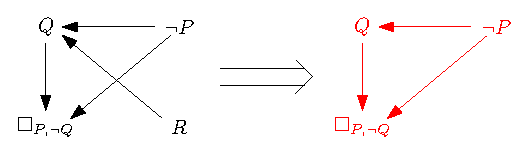
\includegraphics[width=0.5\textwidth ]{images/conflict_graph.eps}
\end{center}
Let $choiceList(G^{conf})$ to be the set of all the choice literals in the conflict graph, given $\Delta$, if we set as true\footnote{
    We recall that a literal $l$ can be an atom or a negated atom. If $l=P$ where $P$ is an atom, setting $l$ to true means $l=P=1$, if $l=\lnot P$, setting $l$ to true means $l=1=\lnot P\implies P=0$. 
} all the literals in $choiceList(G^{conf})$ we will have a false statement:\begin{equation}
    \Delta\models \left( \bigwedge_{l\in 
    choiceList(G^{conf})} l \right)\rightarrow \bot
\end{equation}
This can be rewritten as\begin{equation}
    \Delta\models \bigwedge_{l\in 
    choiceList(G^{conf} )\lnot l}
\end{equation}
\begin{proposition}[Clause Learning]
    Let $\Delta$ to be a set of clauses and let $G^{conf}$ be a conflict graph at some time point during a run of DPLL on $\Delta$. Let $choiceList(G^{conf})$ to be the set of all the choice literals in the conflict graph, then\begin{equation}
        \Delta\models\{\lnot l \ | \ l\in choiceList(G^{conf})\}
    \end{equation}
    The negation of the choice literals in a conflict graph is a valid clause.
\end{proposition}
So during the execution of the DPLL we can analyze a conflict graph and derive a new clause \begin{equation}
    C=\{\lnot l \ | \ l\in choiceList(G^{conf})\}
\end{equation}
we can add $C$ into $\Delta$ and retract the last choice literal $l'$.
\subsubsection{Example}
Let $$\Delta=\{\{\lnot A,\lnot B\},\{\lnot A,B\}\}$$
we apply the DPLL and set in a branch $A=1$ so
$$\{\{\lnot B\},\{B\}\}$$
we have a conflict and the new clause derived by negating the choice literals is\begin{equation}
    C=\{\lnot A\}
\end{equation}
Now we add this to the set of clauses and we have 
$$\Delta=\{\{\lnot A,\lnot B\},\{\lnot A,B\}, \{\lnot A\}\}$$
Now the algorithm instantly knows that $A$ must be False and will no longer waste time proving $A = 1$.\bigskip 

After adding the new clause $C$, the process follows three fundamental logical phases to avoid repeating the same mistake:\begin{enumerate}
    \item The algorithm retracts the last choice made, denoted as $l'$ ( the truth value assigned to $l'$ is removed and it becomes an unassigned literal again). This is necessary because the combination of previous choices ($l_1, \dots, l_k$) together with $l'$ has just been shown to be inconsistent.
    \item  once $C$ is added and the $l'$ choice is cancelled, the $C$ clause becomes a unit clause (only one unassigned literal remains). In this case, $\lnot l'$ is no longer a ''free choice'' of the algorithm, but becomes a literal implied by Unit Propagation (UP).
    \item The algorithm reruns Unit Propagation and continues the analysis. If a new conflict were to occur, the learned clause will be even more ''powerful'' because it will only contain the even older choices ($l_1, \dots, l_k$), allowing you to move up the decision hierarchy.
\end{enumerate}
We saw how the original DPLL algorithm generates proof  exponentially
 longer than their shortest (general) resolution proof. This is not true with clause learning, that renders DPLL equivalent to full resolution.

 \section{Predicate Logic (FOL)}
A logic is a family of formal languages, which has the purpose of \textit{representing} information and 
\textit{manipulate} knowledge. Each logic is provided with a \textbf{syntax} and a \textbf{semantics}, the syntax 
defines a series of symbols and the structure that the formulas must take on to be considered valid, the semantics 
defines the meaning of these formulas.\acc 
In classical logic, each formula, based on the ''world'' to which it is applied, can be true or false. 
To define the syntax I must establish:\begin{itemize}
    \item What symbols can I use (the alphabet)
    \item Which finite sequences of symbols can compose a formula
\end{itemize}
Semantics, on the other hand, establishes the \textit{truth} of formulas in the so-called possible ''worlds'', i.e 
the \textbf{interpretations}. In first-order logic, also called \textbf{FOL}, one establishes\begin{itemize}
    \item Syntax 
    \item Semantics \begin{itemize}
        \item Interpretation 
        \item Variable assignment 
        \item Model 
        \item Evaluating a formula 
    \end{itemize}
    \item Satisfaction 
    \item Unsatisfiability
    \item Validity
\end{itemize}
 \subsection{Syntax}
In a FOL formula there are:\begin{itemize}
    \item Variables: $x,x_1,x_2,x',x''\dots$
    \item True ($\top$) or False $(\bot)$ symbols 
    \item Operators: $\lnot,\land,\lor,\rightarrow,\leftrightarrow$
    \item Quantifiers: $\forall,\exists$
\end{itemize}
We can have constant symbols that represents an object\begin{equation}
    BlockA, BlockB, a, b
\end{equation}
predicate symbols that returns true or false taking an object as an input:\begin{equation}
    Block(.), Above(.,.)
\end{equation}
The arity (number of argument) can be $\ge 1$. For example:\begin{equation}
    Chase(Cat,Mouse)=\top 
\end{equation}
Means that the cat chase the mouse. Then we have the function symbols:\begin{equation}
    WeightOf(.), Succ(.), Sum(.,.)
\end{equation}
these functions returns an object and not a truth value\begin{equation}
    Sum(3,4)=7
\end{equation}
where $3,4$ and $7$ are constant symbols. Constant symbols are just function symbols of arity zero.\begin{definition}[Signature]
    A signature $\Sigma$ in predicate logic is a finite set
 of constant symbols, predicate symbols, and function symbols.
\end{definition}
Another example of formula is\begin{equation}
    \forall x[Dog(x)\rightarrow \exists y Chase(x,y)]
\end{equation}
Means: For every $x$ such that $x$ is a dog, there exists something ($y$) such that $x$ chase $y$, in a few words: Every
 dog chases something.\begin{definition}[Term]
    Let $\Sigma$ to be a signature:\begin{itemize}
        \item every variable and every constant symbol is a term.
        \item if $t_1\dots,t_n$ are terms and $f$ is a $n$-ary function symbol, then $f(t_1\dots,t_n)$ is a term.
    \end{itemize}
 \end{definition}
 \begin{definition}[Atoms]
     Let $\Sigma$ to be a signature:\begin{itemize}
        \item $\top$ and $\bot$ are atoms
        \item if $t_1\dots,t_n$ are terms and $P$ is a $n$-ary predicate symbol, then $P(t_1\dots,t_n)$ is an atom.
     \end{itemize}
 \end{definition}
 \begin{definition}[Formula]
     Let $\Sigma$ to be a signature:\begin{itemize}
        \item each atom is a formula. 
        \item if $\varphi$ is a formula, $\lnot \varphi$ is a formula 
        \item if $\varphi$ and $\psi$ are formulas then\begin{itemize}
    \item $\varphi\land \psi$ is a formula (\textit{conjunction})
    \item $\varphi\lor \psi$ is a formula (\textit{disjunction})
    \item $\varphi\rightarrow \psi$ is a formula (\textit{implication})
    \item $\varphi\leftrightarrow \psi$ is a formula (\textit{equivalence})
\end{itemize}
    \item if $\varphi$ is a formula and $x$ a variable then\begin{itemize}
        \item $\forall x\varphi$ is a formula
        \item $\exists x\varphi$ is a formula
    \end{itemize}
     \end{itemize}
 \end{definition}
 Generally:\begin{itemize}
    \item terms represents object 
    \item predicates represents relations on the universe
 \end{itemize}
 \begin{definition}[Interpretation]
    Let $\Sigma$ be a signature. A $\Sigma$-interpretation is a pair $(U, I)$ where $U$, the universe, is an arbitrary non-empty set $$U = \{o_1, o_2, \dots\}$$ and $I$ is a function, notated as superscript, so that:\begin{enumerate}


    \item$I$ maps constant symbols to elements of $U$: $c^I \in U $ $$ Lassie^I = o_1$$
    \item$I$ maps $n$-ary predicate symbols to $n$-ary relations over $U$:$P^I \subseteq U^n $ $$ Dog^I = \{o_1, o_3\}$$
    \item$I$ maps $n$-ary function symbols to $n$-ary functions over $U$:$f^I \in [U^n \mapsto U]$ $$FoodOf^I = \{(o_1 \mapsto o_4), (o_2 \mapsto o_5), \dots\}$$\end{enumerate} 
    
    We will often refer to $I$ as the interpretation, omitting $U$. Note that $U$ may be infinite.
 \end{definition}
 \begin{definition}[Ground Term Interpretation]
    The interpretation of a ground term under $I$ is $$(f(t_1, \dots, t_n))^I = f^I(t_1^I, \dots, t_n^I)$$
 \end{definition}
 \begin{definition}[Ground Atom Satisfaction]
    Let $\Sigma$ be a signature and $I$ a $\Sigma$-interpretation. We say that $I$ satisfies a ground atom $P(t_1, \dots, t_n)$, written $I \models P(t_1, \dots, t_n)$, iff $(t_1^I, \dots, t_n^I) \in P^I$. We also call $I$ a model of $P(t_1, \dots, t_n)$.
$$ 
I \models Dog(Lassie) \text{ because } Lassie^I = o_1 \in Dog^I
$$
 \end{definition}
 \textbf{Example} ''Integers'': $$U = \{1, 2, 3, \dots\}$$ $$1^I = 1, 2^I = 2, 3^I = 3, \dots$$$$Even^I = \{2, 3, 4, 6, \dots\}$$ $$Equals^I = \{\langle 1, 1 \rangle, \langle 2, 2 \rangle, \dots\}$$ $$Succ^I = \{(1 \mapsto 2), (2 \mapsto 3), \dots\}$$
 \begin{definition}[Variable Assignment]
    Let $\Sigma$ be a signature and $(U,I)$ an interpretation. Let $X$ be the set of all variables. A variable assignment $\alpha$ is a
 function $\alpha : X\mapsto U$. 
 \end{definition}
\begin{definition}[Term Interpretation]
The interpretation of a term under $I$ and $\alpha$ is:
\begin{enumerate}
    \item $x^{I,\alpha} = \alpha(x) \quad [x^{I,\alpha} = o_1]$
    \item $c^{I,\alpha} = c^I \quad [Lassie^{I,\alpha} = Lassie^I]$
    \item $(f(t_1, \dots, t_n))^{I,\alpha} = f^I(t_1^{I,\alpha}, \dots, t_n^{I,\alpha})$ 
\end{enumerate}
\end{definition}
\begin{definition}[Atom Satisfaction]
Let $\Sigma$ be a signature, $I$ a $\Sigma$-interpretation, and $\alpha$ a variable assignment. We say that $I$ and $\alpha$ satisfy an atom $P(t_1, \dots, t_n)$, written $I, \alpha \models P(t_1, \dots, t_n)$, if and only if $(t_1^{I,\alpha}, \dots, t_n^{I,\alpha}) \in P^I$. We also call $I$ and $\alpha$ a model of $P(t_1, \dots, t_n)$.
\end{definition}
From now, we write $\alpha\frac{x}{o}$ to overwrite $x$ with $o$ in $\alpha$.
\begin{definition}[Formula Satisfaction]
Let $\Sigma$ be a signature, $I$ a $\Sigma$-interpretation, and $\alpha$ a variable assignment. We set:
\begin{align*}
    &I, \alpha \models \top \quad \text{and} \quad I, \alpha \not\models \bot \\
    &I, \alpha \models \neg \varphi \quad \text{iff} \quad I, \alpha \not\models \varphi \\
    &I, \alpha \models \varphi \wedge \psi \quad \text{iff} \quad I, \alpha \models \varphi \text{ and } I, \alpha \models \psi \\
    &I, \alpha \models \varphi \vee \psi \quad \text{iff} \quad I, \alpha \models \varphi \text{ or } I, \alpha \models \psi \\
    &I, \alpha \models \varphi \rightarrow \psi \quad \text{iff} \quad \text{if } I, \alpha \models \varphi, \text{ then } I, \alpha \models \psi \\
    &I, \alpha \models \varphi \leftrightarrow \psi \quad \text{iff} \quad I, \alpha \models \varphi \text{ if and only if } I, \alpha \models \psi \\
    &I, \alpha \models \forall x \varphi \quad \text{iff} \quad \text{for all } o \in U \text{ we have } I, \alpha \frac{x}{o} \models \varphi \\
    &I, \alpha \models \exists x \varphi \quad \text{iff} \quad \text{there exists } o \in U \text{ so that } I, \alpha \frac{x}{o} \models \varphi
\end{align*}
If $I, \alpha \models \varphi$, we say that $I$ and $\alpha$ satisfy $\varphi$ (are a model of $\varphi$).
\end{definition}
Like the propositional logic, a formula can be\begin{itemize}
    \item  satisfiable if there exist $I,\alpha$ that satisfy $\varphi$.
    \item unsatisfiable if $\varphi$ is not satisfiable.
    \item falsifiable if there exist $I,\alpha$ that do not satisfy $\varphi$.
    \item valid if $I,\alpha\models\varphi$ holds for all I and $\alpha$. We also call $\varphi$ a tautology.
\end{itemize}
\begin{definition}
    Given two formulas $\varphi,\psi$, we say that $\varphi$ \textbf{entails} $\psi$ $$ \varphi\models\psi$$ if every model of $\varphi$ is also a model of $\psi$. If $$\varphi\models\psi\land \psi\models\varphi $$
    then the two formulas are \textbf{equivalent}:$$ \varphi\equiv\psi$$
\end{definition}
Let's consider the formula:\begin{equation}
    \varphi=\forall x [R(x,y)]
\end{equation}
the variable $y$ is called \textit{free}, so the formula is not closed and cannot be evaluated in a truth value. We define the \textbf{Knowledge Base} as a set $KB$ of closed formulas.
\subsection{Normal Forms}
It is convenient to express the FOL formulas in normal forms to describe the problem. \bigskip

\noindent The \textbf{Prenex normal form} move all the quantifiers at the beginning of the formula, the following rules must be applied (STEP 1):\begin{enumerate}
    \item Eliminate $\leftrightarrow$: $(\varphi\leftrightarrow\psi)\equiv [(\varphi\rightarrow\psi)\land(\psi\rightarrow\varphi)]$
    \item Eliminate $\rightarrow$: $(\varphi\rightarrow\psi)\equiv (\lnot\varphi\lor\psi)$
    \item Apply De Morgan: \begin{itemize}
        \item $\lnot(\varphi\land\psi)\equiv (\lnot \varphi\lor\lnot\psi)$
        \item $\lnot(\varphi\lor\psi)\equiv (\lnot \varphi\land\lnot\psi)$
    \end{itemize}
    \item Move $\lnot$ inwards: \begin{itemize}
        \item $\lnot \forall x \varphi \equiv \exists x \lnot \varphi$
        \item $\lnot\exists x \varphi\equiv \forall x \lnot \varphi$
    \end{itemize}
\end{enumerate}
Let's see an example of application:\begin{align*}
    &\lnot\forall x[(\forall x P(x))\blueText{\rightarrow} R(x)]\equiv\\
    &\blueText{\lnot\forall} x[\lnot(\forall x P(x))\lor R(x)]\equiv\\
    &\exists x \blueText{\lnot}[\lnot (\forall xP(x))\lor R(x) ]\equiv\\
    &\exists x [ (\forall xP(x))\land \lnot R(x) ]
\end{align*}
The general form of a Prenex normal form formula is\begin{equation}
    Qx_1Qx_2\dots Qx_n\varphi 
\end{equation}
where $Q\in \{\forall,\exists\}$ is a generic quantifier. After applying the first set of rules, the following must be applied (STEP 2):\begin{itemize}
    \item if $x$ is not free in $\psi$: $$ 
    (\forall x\varphi)\land \psi \equiv \forall x(\varphi\land\psi)
    $$
    $$ 
    (\forall x\varphi)\lor \psi \equiv \forall x(\varphi\lor\psi)
    $$
    $$ 
    (\exists x\varphi)\land \psi \equiv \exists x(\varphi\land\psi)
    $$
    $$ 
    (\exists x\varphi)\lor \psi \equiv \exists x(\varphi\lor\psi)
    $$
\end{itemize}
\begin{definition}
    If $x$ is a variable, $t$ a term and $\varphi$ a formula, then the \textbf{instantiation} of $x$ with $t$ in $\varphi$, written $ \varphi\frac{x}{t}$, replace all free appearances of $x$ in $\varphi$ by $t$. If $t=y$ is a variable, then $\varphi\frac{x}{y}$ just renames the variable $x$ with $y$.
\end{definition}
\begin{lemma2}
    if $y$ is a variable that doesn't appears in $\varphi$, then\begin{align*}
        &\forall x \varphi\equiv \forall y \varphi\tfrac{x}{y}\\ 
        &\exists x \varphi\equiv \exists y \varphi\tfrac{x}{y}
    \end{align*}
\end{lemma2}
This Lemma is useful to move outwards the variable like in the following example:\begin{align*}
    &\exists x [ (\blueText{\forall xP(x)})\land \lnot R(x) ]\equiv\\ 
     &\exists x [ (\blueText{\forall yP(y)})\land \lnot R(x) ]\equiv\\
     &\exists x\forall y [ P(y)\land \lnot R(x) ]
\end{align*}
\begin{theorem}
    There exists an algorithm that, for any FOL formula $\varphi$, calculates in polynomial time an equivalent formula in Prenex normal form.
\end{theorem}
The \textbf{Skolem normal form} is a formula (that is also in Prenex normal form) where each quantifier is universal:\begin{equation}
    \forall x_1\forall x_2\dots\forall x_n\varphi
\end{equation}
Each formula in Prenex normal form can be easily transformed, consider the following theorem.\begin{theorem}[Skolem]
    Let $\varphi=\forall x_1\forall x_2\dots \forall x_k\exists y\psi$ to be a closed FOL formula in Prenex normal form such that, all the variables are pairwise distinct
    $$x_i\ne x_j, \ \forall i\ne j $$
    let $f$ to be a $k$-ary function symbol ($k$ can also be zero i.e. $f$ is constant) that doesn't appear in $\varphi$. $\varphi$ is satisfiable if and only if the formula\begin{equation}
       \forall x_1\forall x_2\dots \forall x_k\psi\tfrac{y}{f(x_1\dots x_k)}
    \end{equation}
\end{theorem}
Let's see an example of application of the theorem. We consider 
$$ \exists x\forall y \exists z R(x,y,z)$$
we remove $\exists x$ using the theorem:\begin{align*}
     &\exists x\forall y \exists z R(x,y,z)\equiv  \blueText{\exists x}[\forall y \exists z R(x,y,z)]\equiv
\end{align*}
Now the formula have the form $\exists x\varphi$ so we can substitute $x$ with a $0$-arity function (a constant).
\begin{align*}
      &\forall y \exists z R(\blueText{f},y,z)
\end{align*}
By applying the theorem again we can substitute $z$ with a function $g$ of arity 1 in the variable $y$:
\begin{align*}
      &\forall y R(f,y,\blueText{g(y)})
\end{align*}
In this way a Prenex formula can be transformed in a Skolem formula.
\begin{theorem}
    There exists an algorithm that, for any closed FOL formula $\varphi$, efficiently calculates a Skolem normal form formula that is satisfiable if and only if $\varphi$ is satisfiable.
\end{theorem}
If $\varphi$ is a FOL formula, their relative Skolem formula is denoted $\varphi^*$. The theorem says that:\begin{quotation}
    \textit{Satisfying existential quantifier for universally quantified variables $x_1\dots x_k$ is equivalent to choose a value for a function of $x_1\dots x_k$.}
\end{quotation}
Like the Skolem normal form it is a specialization of the Prenex normal form, the \textbf{Clausal normal form} is a specialization of the Skolem normal form. A formula is in this normal form if has the following structure:\begin{equation}
    \forall x_1\forall x_2\dots \forall x_n(l_1\lor \dots \lor l_n)
\end{equation}
where $l_i$ are literals that (may) depends on $x_1\dots x_n$ (the formula must be closed). Any Skolem formula can be transformed in a Clausal formula\begin{enumerate}
    \item consider $ \forall x_1\forall x_2\dots \forall x_n \varphi$
    \item transform $\varphi$ to a SAT-equivalent CNF formula $\psi$
    \item write a set of clauses, one for each disjunction in $\psi$
    \item renames the variables so that each occurs in at most one clause.
\end{enumerate} 
\begin{theorem}
    There exists an algorithm that, for any closed FOL formula $\varphi$,
 efficiently calculates a formula in clausal normal form that is satisfiable if and only if
 $\varphi$ is satisfiable.
\end{theorem}
\subsection{FOL Via Propositional Logic}
In this section we consider a way to reason about FOL using propositional logic, in particular, we bring a FOL formula in SNF (Skolem normal form) and then we generate a \textit{Herbrand expansion}\footnote{We will define it later} to use propositional reasoning.\bigskip

For any finite set of FOL formulas $\theta^*$, we denote $CF(\theta^*)$ the set of constant symbols and function occurring in $\theta^*$. If no constant symbols occurs in $\theta^*$ we add a new ''virtual'' symbol $c$ in $CF(\theta^*)$.
\begin{definition}[Herbrand Universe]
    Given a set of FOL formulas $\theta^*$ in SNF, the Herbrand Universe $HU(\theta^*)$ over $\theta^*$ is the set of all the \textbf{ground terms} that can be formed from $CF(\theta^*)$. 
\end{definition}
We recall what is a ground term:\begin{itemize}
    \item if $a$ is a constant term (function of arity $0$), then $a$ is a ground term 
    \item if $a_1,\dots a_k$ are ground terms and $f$ is a function of arity $k$, then $f(a_1,\dots a_k)$ is a ground term.
\end{itemize}
For example let\begin{equation}
    \theta^*=\{\forall x[\lnot Dog(x)\lor Chases(x,f(x))]\}
\end{equation}
then $CF(\theta^*)=\{c,f\}$ and\begin{equation}
    HU(\theta^*)=\{c,f(c),f(f(c)), f(f(f(c)))\dots \}
\end{equation}
Notice how $HU(\theta^*)$ is infinite in general.
\begin{definition}[Herbrand Expansion]
    Given a set of FOL formulas $\theta^*$ in SNF, the Herbrand expansion $HE(\theta^*)$ is the following set of formulas:\begin{equation}
        HE(\theta^*)=\left\{
            \varphi\tfrac{x_1}{t_1}\dots \tfrac{x_n}{t_n} \ | \ (\forall x_1\dots \forall x_n\varphi)\in \theta^* \ \land \ t_i\in HU(\theta^*)
        \right\}
    \end{equation}
\end{definition}
We are instantiating each possible formula $\varphi$ from the terms in $HU(\theta^*)$ that contains ground terms, so it can be interpreted as propositional logic.
\begin{theorem}[Herbrand]\label{teo:Herbrand}
    A set of FOL formulas in SNF $\theta^*$ is satisfiable\footnote{
       A set of formulas is said to be satisfiable if there exists at least one interpretation (called model) which simultaneously makes all the formulas in the set true.
    }
    if and only if the entire set $HE(\theta^*)$ is satisfiable (all the propositional logic formulas in $HE(\theta^*)$ can be satisfied simultaneously by a model.)
\end{theorem}
Notice how, without function symbols of arity greater than 0, the Herbrand expansion is finite, and the FOL reasoning is \textit{equivalent} to propositional reasoning.
\begin{theorem}[Compactness of Propositional Logic]\label{propCompact}
Any set $\theta$ of
propositional logic formulas is unsatisfiable if and only if at least one
finite subset of $\theta$ is unsatisfiable.
\end{theorem}
We can enumerate all finite subsets $\theta_1$ of the Herbrand expansion $HE(\theta^*)$ and test propositional satisfiable of $\theta_1$, $\theta$ is unsatisfiable if and only if one of the subsets $\theta_1$ is unsatisfiable.\begin{quote}
    \textit{
        If the Herbrand expansion is infinite, to show unsatisfiability, we must somehow choose a ''relevant'' finite subset thereof.
    }
\end{quote}
\begin{theorem}
    The set of unsatisfiable FOL formulas is recursively
 enumerable.
\end{theorem}
\textit{Proof}:  Enumerate all FOL formulas $\varphi$. Incrementally for all of these in parallel,
enumerate all finite subsets $\theta_1$ of the Herbrand expansion $HE(\theta^*)$. Test
propositional satisfiability of each  $\theta_1$. By compactness of propositional logic, if
$HE(\theta^*)$ is unsatisfiable then one of the  $\theta_1$ is.
\hfill$\blacksquare$
\begin{theorem}
    The problem of establishing whether a FOL formula is satisfiable or not is undecidable.
\end{theorem}
\begin{corollary}
    The set of satisfiable FOL formulas is not recursively enumerable.
\end{corollary}
\begin{quotation}
    \textit{
        If a FOL formula is unsatisfiable, then we can confirm this. Otherwise, we might end up in an infinite loop.
    }
\end{quotation}
\section{FOL Resolution}
\subsection{Substitution and Unification}
Consider the Clausal normal form\begin{equation}
    \forall x_1\forall x_2\dots \forall x_n(l_1\lor \dots \lor l_n)
\end{equation}
we can write a form of that structure by omitting the quantifiers in the following notation:\begin{equation}
    \{l_1,\dots l_n\}
\end{equation}
The idea is to ''adapt'' the propositional resolution rule 
\begin{equation}
    \frac{C_1\dot\cup\{l\},C_2\dot\cup\{\lnot l\}}{C_1\cup C_2}
\end{equation}
to the first order logic.
\begin{definition}[Substitution]
    A \textbf{Substitution} $s=\{\tfrac{x_1}{t_1}\dots \tfrac{x_n}{t_n}\}$ is a function that substitutes the variables $x_i$ for terms $t_i$ where $x_i\ne t_i$ for all $i$. Given a formula $\varphi$, we denote $\varphi s$ the application of $s$ on $\varphi$, which is $\varphi$ with all occurrences of $x_i$ simultaneously replaced by $t_i$.
\end{definition}
\begin{quotation}
    Variable instantiation and renaming, as used in the prenex and Skolem
 transformations as well as in the Herbrand expansion, is a special case of
 substitution.
\end{quotation}
for example, given $s=\{\tfrac{x}{y},\tfrac{y}{h(a,b)}\}$:\begin{equation}
    P(x,y)s=P(y,h(a,b))
\end{equation}
\begin{definition}[Composition]
    Given two substitutions $s_1,s_2$ we denote $s_1s_2$ the \textbf{composed substitution} that is the single subsection identical to $s_2\circ s_1$ (apply $s_1$ then $s_2$).
\end{definition}
For example, given $s_1=\{\tfrac{z}{g(x,y)},\tfrac{v}{w}\}$ and $s_2=\{\tfrac{x}{a},\tfrac{y}{b},\tfrac{w}{v},\tfrac{z}{d}\}$ we have\begin{equation}
    P(x,y,z,v)s_1s_2=P(x,y,g(x,y),w)s_2=P(a,b,g(a,b),v)
\end{equation}
Given $s_1$ and $s_2$ to get $s_1s_2$ we can\begin{enumerate}
\item replace all the terms $t_i$ in $s_1$ by applying $s_2$\item then for any variable $x_i$ replaced by $s_2$ but not by $s_1$, apply the
respective variable/term pair $\tfrac{x_i}{t_i}$ of $s_2$\item remove any pairs of variable $x$ and term $t$ where $x=t$.\end{enumerate} 
For any formula $\varphi$ and triplets of substitutions $s_1,s_2,s_3$, the following properties holds:\begin{enumerate}
    \item $(\varphi s_1)s_2=\varphi(s_1s_2)$
    \item $(s_1s_2)s_3=s_1(s_2s_3)$
    \item $s_1s_2\ne s_2s_1$ in general.
\end{enumerate}
A substitution $s=\{\tfrac{x_1}{t_1}\dots \tfrac{x_n}{t_n}\}$ is idempotent $$\varphi ss=\varphi s$$ if $t_i$ does not contain $x_j$ for all $i,j$.
\begin{definition}[Unifier]
    A substitution $s$ is a \textbf{unifier} for a set of expressions $\{E_i\}=\{E_1\dots E_k\}$ if $E_is=E_js$ forall $i,j$.
\end{definition}
\begin{definition}
    A substitution $g$ that is a unifier for $\{E_i\}$ is the \textbf{most general unifier (mgu)} if, for any $s$ unifier for $\{E_i\}$, there exists an other $s'$ unifier for $\{E_i\}$ such that \begin{equation}
        \{E_i\}s=\{E_i\}gs'.
    \end{equation}
\end{definition}
\begin{proposition}
    If any unifier exists, then an idempotent mgu exists.
\end{proposition}
We want to define an algorithm that finds the mgu for a set of expressions $\{E_i\}$.
\begin{proposition}
    If the only way to unify $\{E_i\}$ is to unify a variable $x$ with a term $t$ that contains $x$, then, $\{E_i\}$  cannot be unified.
\end{proposition}
We call a \textbf{disagreement set} of a set of expressions $\{E_i\}$, the set of sub-expressions $\{t_i\}\subseteq \{E_i\}$ at the first position of  $\{E_i\}$ for which some of the $\{E_i\}$ disagree. For example with 

\[ P(x,c,f(y)), P(x,z,z) \text{ have the disagreement set: }\{c,z\}\]
since $c$ and $z$ are the first terms on which the expressions in $\{E_i\}$ disagree. Another example is 
\[\{P(x,a,f(y)),P(y,a,f(y))\}\]
the expressions disagree on the first term\begin{align*}
    &P(\blueText{x},a,f(y))\\
    &P(\blueText{y},a,f(y))\implies\\
    &\text{disagreement set: }\{x,y\}
\end{align*}
We use this definition to build an algorithm that returns a unifier for a set of expressions (if any).
\begin{theorem}
    The Algorithm \ref{alg:mgu} succeeds if and only if there is a unifier for $\{E_i\}$. In the positive case, the algorithm returns an idempotent mgu of $\{E_i\}$.
\end{theorem}
\begin{algorithm}
\caption{Find-MGU}\label{alg:mgu}
\begin{algorithmic}[1]
\State given $\{E_i\}$
\State $k\leftarrow 0, \ T_k\leftarrow \{E_i\}, \ s_k\leftarrow \{\}, \ $
\While{$T_k$ is not a singleton}
\State Let $D_k$ be the disagreement set of $T_k$
\State \blueText{/*if $t_k$ contains $x_k$ the unification is impossible*/}
\State Let $x_k,t_k\in D_k$ be a variable and term such that $t_k$ does not contain $x_k$
\If{such $x_k,t_k$ does not exists} 
\State\Return failure
\EndIf
\State $s_{k+1}\leftarrow s_k\{\tfrac{x_k}{t_k}\}$ \blueText{/*$t_k$ does not contain any of $x_1\dots x_k$*/}
\State $T_{k+1}\leftarrow T_k\{\tfrac{x_k}{t_k}\}$ \blueText{/*$x_k$ does not occur in $T_{k+1}$*/}
\State $k\leftarrow k+1$
\EndWhile 
\State\Return $s_k$
\end{algorithmic}
\end{algorithm}
Let's see an example of application, the input set is\[\{P(x,f(y),y),P(z,f(b),b)\}\]
At the first iteration with $k=0$ we have \begin{align*}
    &D_0=\{x,z\}\\ 
    &\text{select $x$ and $z$ in $D_0$ since $z$ does not contain $x$}\\
    &s_1=\{\tfrac{x}{z}\}\\ 
    &\text{we substitute $x$ with $z$ in the set of expressions}\\ 
    &\{P(\blueText{x},f(y),y),P(z,f(b),b)\}\implies \{P(\blueText{z},f(y),y),P(z,f(b),b)\}\\ 
    &T_1=\{P(z,f(y),y),P(z,f(b),b)\}
\end{align*}
at the second iteration with $k=1$ we have \begin{align*}
    &D_1=\{y,b\}\\
    &s_2=s_1\{\tfrac{y}{b}\}=\{\tfrac{x}{z},\tfrac{y}{b}\}\\
    &T_2=\{P(z,f(b),b),P(z,f(b),b)\}=\{P(z,f(b),b)\}
\end{align*}
at this point $T_2$ contains a single element so the output will be $s_2=\{\tfrac{x}{z},\tfrac{y}{b}\}$.\bigskip 

Now we explain in the details the FOL resolution, we assume that the formulas are in Clausal normal form:\begin{equation}
    \forall x_1\dots \forall x_n(l_1\lor \dots \lor l_n)
\end{equation}
written\begin{equation}
    \{l_1,\dots l_n\}
\end{equation}
we recall that a clause is a set of disjunction of literal, a set of clause is denoted $\Delta$, the empty clause is denoted $\square$ and a \textit{calculus} is a set of inference rules.
\begin{definition}[Derivation]
    Given a set of clause $\Delta$ we say that a clause $C$ can be \textbf{derived} from $\Delta$ using a calculus $\mathcal R$, written \[\Delta\models_{\mathcal R}C\]
    if, starting from $\Delta$ we can apply a sequence of rule from $\mathcal R$ ending in $C$.
\end{definition}
We recall the following properties\begin{itemize}
    \item A calculus $\mathcal R$ is \textbf{sound} if $\Delta\models_{\mathcal R}C\implies \Delta\models C$. Soundness assures you that the derivation system $\mathcal R$  is ''reliable'', and that the clause it derives are logically correct with respect to $\Delta$.
    \item A calculus $\mathcal R$ is \textbf{resolution complete} if $\Delta\models \bot$ implies $\Delta\models_{\mathcal R}\square$, i.e. if $\Delta$ is unsatisfiable is possible to derive the empty clause from it with $\mathcal R$.
\end{itemize}
We remind that to decide whenever $KB\models \varphi$ we can check the satisfiability of $\psi = KB\cup\{\varphi\}$. If this is unsatisfiable then $KB\models \varphi$. So the idea is\begin{itemize}
    \item to check if $KB\models \varphi$ we consider $KB\cup\{\varphi\}$
    \item we try to derive the empty clause $\square$ from $KB\cup\{\varphi\}$.
\end{itemize}
Now let's see our resolution rule.
\begin{definition}[Propositional Resolution]
    The resolution uses the following resolution rule:\begin{equation}
        \frac{C_1\dot\cup\{l\},C_2\dot\cup\{\lnot l\}}{C_1\cup C_2}
    \end{equation}
\end{definition}
So, if $\Delta$ contains two clauses of the form\[C_1\dot\cup\{l\},C_2\dot\cup\{\lnot l\}\]
the rule derive the new clause $C_1\cup C_2$, $l$ and $\lnot l$ are called resolution literals. 
\begin{definition}[Binary FOL Resolution]
    The resolution uses the following resolution rule:\begin{equation}
        \frac{C_1\dot\cup\{P_1\},C_2\dot\cup\{\lnot P_2\}}{[C_1\cup C_2]g}
    \end{equation}
    where $g$ is the mgu.
\end{definition}
If $\Delta$ contains two clauses of the form 
$$\{C_1\dot\cup\{P_1\},C_2\dot\cup\{\lnot P_2\}\}$$
where $P_1$ and $P_2$ \textbf{can be unified} and $g$ is an mgu for them, the rule allows to derive the clause $[C_1\cup C_2]g$ (the union of $C_1$ and $C_2$ where we apply the unification). $P$ and $\lnot P$ are called resolution literals. The two rules presented satisfies the properties of soundness.
\begin{theorem}
    The calculus with only the binary FOL resolution is not complete.
\end{theorem}
As a proof consider the following example:\begin{equation}
    \Delta=\{
        \{P(x_1,x_2),P(x_2,x_1)\},
        \{\lnot P(y_1,y_2),\lnot P(y_2,y_1)\}
    \}
\end{equation}
this $\Delta$ is not satisfiable, the variables in FOL clauses are universally quantified, to satisfy $\Delta$ we would have to satisfy $P(o,o)$ and $\lnot P(o,o)$ for all the objects $o$ in the universe. We notice that we can't derive the empty clause $\square$ from $\Delta$ using the binary FOL resolution.\bigskip


Now we present two rules that forms a sound and complete calculus.

\begin{definition}[Full FOL Resolution]
    The resolution uses the following resolution rule:
    \begin{equation}
        \frac{C_1\dot\cup\{P_1^1\dots P_1^n\},C_2\dot\cup\{\lnot P_2^1\dots \lnot P_2^n\}}{[C_1\cup C_2]g}
    \end{equation}
    where $\{P_1^1,\dots P_1^n,P_2^1,\dots \lnot P_2^n\}$ can be unified and  $g$ is an mgu for them.
\end{definition}
\begin{definition}[Factoring]
    The resolution uses the following resolution rule:\begin{equation}
        \frac{C_1\dot\cup\{l_1\}\dot\cup\{l_2\}}{
            [C_1\cup\{l_1\}]g
        }
    \end{equation}
    where $l_1$ and $l_2$ can be unified and $g$ is an mgu for them. $[C_1\cup\{l_1\}]g$ is a \textbf{factor} of the parent clause.
\end{definition}
We denote $\mathcal{R}_{FactBin}$ the calculus with the factoring rule and $\mathcal{R}_{Full}$ the calculus with the full FOL resolution.
\begin{lemma2}[Lifting Lemma]\label{lemma:lifting}
    Let $C_1$ and $C_2$ be two clauses with no shared variables, and let $C_1^g$ and $C_2^g$ be ground instances of $C_1$ and $C_2$. Say that $C^g$ is a resolvent of $C_1^g$ and $C_2^g$. Then there exists a clause $C$ such that $C^g$ is a ground instance of $C$, and:
\begin{enumerate}
    \item$C$ can be derived from $C_1$ and $C_2$ using $\mathcal{R}_{Full}$.
    \item$C$ can be derived from $C_1$ and $C_2$ using $\mathcal{R}_{FactBin}$.
\end{enumerate}
\end{lemma2}
\begin{theorem}
    The calculus with the full FOL resolution and with the factoring resolution is sound and complete.
\end{theorem}
A sketch of the proof is presented through previous intermediate results:\begin{itemize}
    \item Any set $\theta$ of FOL formula s can be represented in clausal form $\Delta$
    \item we assume that $\Delta$ is unsatisfiable 
    \item we use the \textit{Herbrand} Theorem \ref{teo:Herbrand} and the propositional compactness Proposition \ref{propCompact}, so the (assumed) unsatisfiability of $\Delta$ translates to: some finite set $\Delta'$ of ground instances is unsatisfiable.
    \item by compactness of propositional resolution, we can derive $\square$ from $\Delta'$
    \item $\square$ can also be derived directly from $\Delta$ with the full FOL resolution and the factoring resolution by the lifting Lemma \ref{lemma:lifting}.
\end{itemize}











\chapter{Planning}
Planning (or automatic planning) is a branch of artificial intelligence that deals with generating a strategy or sequence of actions to allow an intelligent agent (such as a robot or software) to achieve an objective starting from an initial state. It's a general way to define a problem solving procedure.
\section{STRIPS}
STRIPS (acronym for STanford Research Institute Problem Solver) is one of the most important automatic planning language and system in the history of artificial intelligence.

Developed in 1971 by Richard Fikes and Nils Nilsson, it was used to control the actions of Shakey, one of the first mobile robots with logical reasoning. In modern terms, STRIPS represents the standard for so-called classic planning.\bigskip 

STRIPS has only boolean variables, the preconditions and the goals are conjunctions of positive atoms, the effects are conjunctions of literals (positive or negated atoms).
\begin{definition}[STRIPS Planning Task]
A \textit{STRIPS planning task}, short \textit{planning task}, is a 4-tuple $\Pi = (P, A, I, G)$ where:

\begin{itemize}
    \item $P$ is a finite set of \textbf{facts} (aka \textbf{propositions}).
    \item $A$ is a finite set of \textbf{actions}; each $a \in A$ is a triple $a = (pre_a, add_a, del_a)$ of subsets of $P$ referred to as the action's \textbf{precondition}, \textbf{add list}, and \textbf{delete list} respectively; we require that $add_a \cap del_a = \emptyset$.
    \item $I \subseteq P$ is the \textbf{initial state}.
    \item $G \subseteq P$ is the \textbf{goal}.
\end{itemize}
\end{definition}
We will often give each action $a \in A$ a \textbf{name} (a string), and identify $a$ with that name.\bigskip

\noindent\textbf{Example: Australian Logistics Planning Task}
\begin{itemize}
    \item \textbf{Facts} $P$: $\{at(x), visited(x) \mid x \in \{Sydney, Adelaide, Brisbane, Perth, Darwin\}\}$.
    \item \textbf{Initial state} $I$: $\{at(Sydney), visited(Sydney)\}$.
    \item \textbf{Goal} $G$: $\{at(Sydney)\} \cup \{visited(x) \mid x \in \{Sydney, Adelaide, Brisbane, Perth, Darwin\}\}$.
    \item \textbf{Actions} $a \in A$: $drive(x, y)$ where $x, y$ have a road.
    \begin{itemize}
        \item \textbf{Precondition} $pre_a$: $\{at(x)\}$.
        \item \textbf{Add list} $add_a$: $\{at(y), visited(y)\}$.
        \item \textbf{Delete list} $del_a$: $\{at(x)\}$.
    \end{itemize}
    \item \textbf{Plan:} $\langle drive(Sydney, Brisbane), drive(Brisbane, Sydney), drive(Sydney, Adelaide),$ 
    $drive(Adelaide, Perth),$\\$ drive(Perth, Adelaide), drive(Adelaide, Darwin),$
    $drive(Darwin, Adelaide), drive(Adelaide, Sydney)\rangle$.
\end{itemize}
 \begin{center}
    \includegraphics[width=0.5\textwidth ]{images/strips_example.png}
\end{center}
\begin{definition}[STRIPS State Space]\label{STRIPS_state_space}
    Let $\Pi = (P, A, c, I, G)$ be a \textit{STRIPS planning task}. The \textit{state space} of $\Pi$ is $\Theta_{\Pi} = (S, A, T, I, S^G)$ where:
\begin{itemize}
    \item The states (also \textbf{world states}) $S = 2^P$ are the subsets of $P$.
    \item $A$ is $\Pi$'s action set.
    \item The transitions are $T = \{s \xrightarrow{a} s' \mid pre_a \subseteq s, s' = (\quadBrack{s}, a)\}$. \\
    If $pre_a \subseteq s$, then $a$ is \textbf{applicable} in $s$ and $$(\quadBrack{s}, a) := (s \cup add_a) \setminus del_a$$ 
    If $pre_a \not\subseteq s$, then $(\quadBrack{s}, a)$ is undefined.
    \item $I$ is $\Pi$'s initial state.
    \item The goal states $S^G = \{s \in S \mid G \subseteq s\}$ are those that satisfy $\Pi$'s goal.
\end{itemize}
\end{definition}
A \textbf{plan} for $s\in S$ is a path from $s$ to $s'\in S^G$, a plan for $I$ is a \textbf{solution} and is called \textit{plan for $\Pi$}, if such plan exists, $\Pi$ is \textbf{solvable}.
 \begin{center}
    \includegraphics[width=0.7\textwidth ]{images/strips_example2.png}
\end{center}
These planning examples draw heavily on the research problems presented in previous chapters, as in this case, it is possible to define a heuristic function that estimates the distance (or cost) between a current state $s$ and the goal state $G$.

It is important to perform a complexity analysis of the problems that we face to identify special cases that can be solved in polynomial time, relax the input into the special case to obtain a heuristic
function.\bigskip
\subsection{Only-Adds STRIPS Tasks}
Let's consider the following example:
\begin{itemize}
    \item \textbf{Facts $P$}: $\{truck(x) \mid x \in \{A, B, C, D\}\} \cup$ \\
    $\{pack(x) \mid x \in \{A, B, C, D, T\}\}$.
    
    \item \textbf{Initial state $I$}: $\{truck(A), pack(C)\}$.
    
    \item \textbf{Goal $G$}: $\{truck(A), pack(D)\}$.
    
    \item \textbf{Actions $A$}: (Notated as ''precondition $\Rightarrow$ adds, $\neg$ deletes'')
    \begin{itemize}
        \item $drive(x, y)$, where $x, y$ have a road: \\
        ''$truck(x) \Rightarrow truck(y), \neg truck(x)$''.
        
        \item $load(x)$: ''$truck(x), pack(x) \Rightarrow pack(T), \neg pack(x)$''.
        
        \item $unload(x)$: ''$truck(x), pack(T) \Rightarrow pack(x), \neg pack(T)$''.
    \end{itemize}
\end{itemize}
 \begin{center}
    \includegraphics[width=0.34\textwidth ]{images/truck.png}
\end{center}
It is clear that this STRIPS planning task models a truck that must collect a package and deposit it in a designated place. One simple relaxation is the following:\begin{quotation}
    \textbf{Only-Adds Relaxation}: Drop the preconditions and deletes on the actions.
\end{quotation}
We want to use this to generate a heuristic function. The general problem is\begin{itemize}
    \item Given a STRIPS task $\Pi = (P, A, I, G)$, we want to find an action sequence $\vec a$ leading from $I$ to a state that contains $G$ when pretending that preconditions and deletes are empty.
\end{itemize}
The simplest possible approach is the following:
\begin{algorithm}
\caption{Solution 1}
\begin{algorithmic}[1]
\State $\vec a=\langle \ \rangle$
\While{$G\ne\emptyset$}
\State select $a\in A$
\State $G=G\backslash add_a$ \blueText{\#Subtract from the remaining objectives anything that the chosen action adds}
\State $\vec a = \vec a \circ \langle a\rangle $
\State $A=A\backslash\{a\}$
\EndWhile
\State\Return $h=|\vec a|$
\end{algorithmic}
\end{algorithm}
This algorithm is applied for each state $s$ and calculates the value of $h$.
This heuristic is not admissible,
admissibility is only guaranteed if we find a
 shortest possible $\vec a$; else, $\vec a$ might be longer than a plan for $\Pi$ itself.
 Selecting an arbitrary action each time, $\vec a$  may be longer than needed. Another solution might be:

 \begin{algorithm}
\caption{Solution 2}
\begin{algorithmic}[1]
\State $\vec a=\langle \ \rangle$
\While{$G\ne\emptyset$}
\State select $a\in A$ such that $|add_a|$ is maximal.
\State $G=G\backslash add_a$ 
\State $\vec a = \vec a \circ \langle a\rangle $
\State $A=A\backslash\{a\}$
\EndWhile
\State\Return $h=|\vec a|$
\end{algorithmic}
\end{algorithm}

$h$ is not admissible yet,  large $add_a$ doesn't help if the intersection with $G$ is small. 


 \begin{algorithm}
\caption{Solution 3}
\begin{algorithmic}[1]
\State $\vec a=\langle \ \rangle$
\While{$G\ne\emptyset$}
\State select $a\in A$ such that $|add_a\cap G|$ is maximal.
\State $G=G\backslash add_a$ 
\State $\vec a = \vec a \circ \langle a\rangle $
\State $A=A\backslash\{a\}$
\EndWhile
\State\Return $h=|\vec a|$
\end{algorithmic}
\end{algorithm}
\bigskip 

Also this is not admissible. To have an admissible (and optimal) heuristic in the relaxed world, we should find the shortest possible sequence of actions ($\text{optimal } \vec{a}$). But finding this sequence is equivalent to solving the Minimum Cover problem, since Minimum Cover is an $\mathsf{NP}$-complete problem, finding the optimal heuristic even for a relaxed problem is computationally expensive.\bigskip 

We call $\mathsf{PlanEx}$ the problem of deciding, given a STRIPS planning task $\Pi$, whether or not there exists a plan for  $\Pi$.
\begin{lemma2}
    $\mathsf{PlanEx}$ is $\mathsf{PSPACE}$-hard.
\end{lemma2}
\textit{Proof Sketch}:
Given a Turing machine with \textbf{space bounded by polynomial $p(|w|)$}, we can in polynomial time (in the size of the machine) generate an equivalent STRIPS planning task. Say the possible symbols in tape cells are $x_1, \dots, x_m$ and the internal states are $s_1, \dots, s_n$, accepting state $s_{acc}$.
\begin{itemize}
    \item The contents of the tape cells: $in(1, x_1), \dots, in(p(|w|), x_1), \dots, in(1, x_m), \dots, in(p(|w|), x_m)$.
    \item The position of the R/W head: $at(1), \dots, at(p(|w|))$.
    \item The internal state of the machine: $state(s_1), \dots, state(s_n)$.
    \item Transitions rules $\mapsto$ STRIPS actions; accepting state $\mapsto$ STRIPS goal $\{state(s_{acc})\}$; initial state obvious.
    \item This reduction to STRIPS runs in polynomial-time because we need only polynomially many facts.
\end{itemize}
\begin{lemma2}
    $\mathsf{PlanEx}$ is in $\mathsf{PSPACE}$.
\end{lemma2}
It is easy and sufficient to prove that $\mathsf{PlanEx}$ is in $\mathsf{NPSPACE}$, since $\mathsf{PSPACE}=\mathsf{NPSPACE}$. From the two lemmas, the following theorems follows.
\begin{theorem}
    $\mathsf{PlanEx}$ is $\mathsf{PSPACE}$-complete.
\end{theorem}
\subsection{Transition System}
The state space of a planning task, like the one described in Definition \ref{STRIPS_state_space}, is generalized in the following definition.\begin{definition}[Transition Systems]
    A transition system is a 6-tuple $\Theta=(S,L,c,T,I,S^G)$ where:\begin{itemize}
        \item $S$ is a finite set of states 
        \item $L$ is a finite set of transition labels (a generalization of an action) 
        \item $c:L\mapsto \R^+\cup\{0\}$ is the cost function
        \item $T\subseteq S\times L\times S$ is the transition relation 
        \item $S^G\subseteq S$ is the set of the goal states.
        \item $I\in S$ is the initial state.
    \end{itemize}
\end{definition}
The size of $\Theta$ is $|S|$. If $\Theta$ has the transition $(s,l,s')\in T$ we write \begin{align*}
    &s\xrightarrow{l}s'
\end{align*}
or \begin{align*}
    &s\xrightarrow{}s'
\end{align*}
if we are not interested in the label $l$. $\Theta$ has unit cost if $c$ is the constant function $c(l)=1, \forall l$.
The classic definitions already addressed follow:\begin{itemize}
    \item $s'$ is a successor of $s$ if $s\rightarrow s'\in T$
    \item $s'$ is a predecessor of $s$ if $s'\rightarrow s\in T$
    \item a path from $s$ to $s'$ is a sequence of transitions:\begin{equation}
        s\xrightarrow{l_1}s_1\xrightarrow{l_2}s_2\dots \xrightarrow{l_n}s_n=s'
    \end{equation}
    and the cost of the path is \begin{equation}
        \sum_{i=1}^nc(l_i)
    \end{equation}
    we say that $s$ is reachable (without specifying the origin) meaning that is reachable from $I$.
\end{itemize}
A solution for $\Theta$ is a path from $I$ to a state $s\in S^G$. If such path exists, $\Theta$ is solvable.
 \begin{center}
    \includegraphics[width=0.6\textwidth ]{images/trans_syst.png}
\end{center}
We are interested in solving \textbf{huge} transition systems (unfeasible to apply Dijkstra), represented in a compact way as planning tasks.
\section{FDR}
STRIPS and FDR (Finite Domain Representation) are two different formalisms for describing planning tasks, both aimed at defining how an agent should move from an initial state to a goal. FDR is a more modern and often more efficient evolution for automatic solvers (like Fast Downward):\begin{itemize}
    \item Finite Domain Variables: Instead of having many Boolean facts (e.g. $truck\_in\_A$, $truck\_in\_B$), use a single multivariate variable (e.g. $TruckPosition$) that can take a value in a finite set $\{A, B, C, D\}$ 
    \item State: A function that assigns a value to each variable.\item Advantage: Reduces the number of ''mutually exclusive'' facts the planner must explicitly handle, making the problem structure clearer.
\end{itemize}


\begin{definition}[FDR  Planning Task]
    A \textit{finite-domain representation planning task}, short \textit{FDR planning task}, is a 5-tuple $\Pi = (V, A, c, I, G)$ where:

\begin{itemize}
    \item $V$ is a finite set of \textit{state variables}, each $v \in V$ with a \textit{finite domain} $D_v$. \\
    We refer to (partial) functions on $V$, mapping each $v \in V$ into a member of $D_v$, as (partial) \textit{variable assignments}.
    
    \item $A$ is a finite set of \textit{actions}; each $a \in A$ is a pair $(pre_a, eff_a)$ of \textit{partial variable assignments} referred to as the action's \textit{precondition} and \textit{effects}.
    
    \item $c: A \mapsto \mathbb{R}^+\cup\{0\}$ is the \textit{cost function}.
    
    \item $I$ is a complete variable assignment called the \textit{initial state}.
    
    \item $G$ is a partial variable assignment called the \textit{goal}.
\end{itemize}
\end{definition}
We say that $\Pi$ has \textit{unit costs} if, for all $a \in A$, $c(a) = 1$. In the FDR context we call \textbf{fact} an assignment$$(v,d)\text{ or }v=d$$
we mean that the variable $v$ assumes the value $d$. 
If $p$ is a partial variable assignment, we write $$ V[p]=\{v\in V \ | \ p(v)\text{ is defined}\}$$
to refers to all variables where $p$ is defined.
For the map example in Australia:
 \begin{center}
    \includegraphics[width=0.3\textwidth ]{images/strips_example.png}
\end{center}
\begin{itemize}
    \item \textbf{Variables $V$}: $at : \{Sydney, Adelaide, Brisbane, Perth, Darwin\}$; $visited(x) : \{T, F\}$ for each city $x$.
    \item \textbf{Initial state $I$}: $at = Sydney, visited(Sydney) = T, visited(x) = F$ for $x \neq Sydney$.
    \item \textbf{Goal $G$}: $at = Sydney, visited(x) = T$ for each $x$.
    \item \textbf{Actions $a \in A$}: $drive(x, y)$ where $x, y$ have a road connecting them.
    \begin{itemize}
        \item Preconditions $pre_a$: $at = x$.
        \item Effects $eff_a$: $at = y, visited(y) = T$.
    \end{itemize}
    \item \textbf{Cost function $c$} (might be a measure of the distance): 
    \[
    c(drive(x, y)) = 
    \begin{cases} 
    1 & \{x, y\} = \{Sydney, Brisbane\} \\
    1.5 & \{x, y\} = \{Sydney, Adelaide\} \\
    3.5 & \{x, y\} = \{Adelaide, Perth\} \\
    4 & \{x, y\} = \{Adelaide, Darwin\} 
    \end{cases}
    \]
\end{itemize}
\begin{definition}[FDR State Space]
    Let $\Pi=(V,A,c,I,G)$ to be an FDR planning task, the \textbf{task space} of $\Pi$ is the labeled transition system $\Theta_\Pi=(S,L,c,T,I,S^G)$ where\begin{itemize}
        \item the states $S$ are all the possible complete variable assignments.
        \item the labels $L=A$ are the actions of $\Pi$, hence, the cost $c$ of $\Pi$ defined on $A$ is equal of the cost $c$ of $\Theta_\Pi$ defined on $L$.
        \item The transitions are\begin{equation}
            T=\{
                s\xrightarrow{a}s' \ | \ a\in A[s], s'= s\quadBrack{a}
            \}
        \end{equation}
        where\begin{itemize}
            \item $A[s]=\{a\in A \ | \ pre_a\subseteq s\}$ are the actions that can be applied in $s$.
            $s\quadBrack{a}$  represents the resulting state after applying the $a$ action.
            $$s\quadBrack{a}=\begin{cases}
                \text{undefined} \text{ if }a\notin A[s]\\ 
                eff_a(v) \text{ if }v\in V[eff_a]\\ 
                s(v) \text{ if }v\notin  V[eff_a]
            \end{cases}$$
        \end{itemize}
    \end{itemize}
\end{definition}

Although the STRIPS language is still used for historical convenience, modern planning systems (such as Fast Downward) prefer to translate everything internally into FDR for reasons of practical efficiency. The FDR format is superior because it reduces unnecessary states, allows you to better map dependencies via causal graphs, and facilitates the creation of more powerful heuristics, offering a much more natural and compact way of modeling reality than the rigid Boolean variables of STRIPS.
\subsection{Conversion between FDR and STRIPS}
An easy way to convert an FDR planning task in a STRIPS planning task is the following\begin{itemize}
    \item for each variable $v$ with domain $\{d_1\dots d_k\}$, we make $k$ STRIPS facts \begin{align*}
        &v=d_1\\ 
        &\vdots \\ 
        &v=d_k
    \end{align*}
\end{itemize}
\begin{definition}
    Let $\Theta=(S,L,c,T,I,S^G)$ and $\Theta'=(S',L',c',T',I',{S'}^G)$ to be two transition systems. We say that $\Theta$ is \textbf{isomorphic} to $\Theta'$ $$ \Theta\sim \Theta'$$
    if there exists two bijective functions $\varphi:S\mapsto S'$ and $\psi:L\mapsto L'$ such that\begin{itemize}
        \item $\varphi(I)=I'$
        \item $s\in S^G$ if and only if $\varphi(s)\in {S'}^G$
        \item $(s,l,t)\in T$ if and only if $(\varphi(s),\psi(l),\varphi(t))\in T'$
        \item for all $l\in L$, $c(l)=c'(\psi(l))$
    \end{itemize}
\end{definition}
Isomorphisms typically result from compilations between different
 formalisms (see later this chapter); we will also sometimes use them as a
 technical device.

 Now we consider a systematic way to convert an FDR planning task in a STRIPS planning task.
 \begin{definition}[FDR to STRIPS]\label{FDR2STRIPS}
    Let $\Pi=(V,A,c,I,G)$ to be an FDR planning task, the \textbf{STRIPS conversion} is the STRIPS planning task $\Pi^{STR}=(P_V,A^{STR},c,I,G)$ where \end{definition}\begin{itemize}
        \item $P_V=\{v=d \ | \ v\in V,d\in D_v\}$ is the set of STRIPS facts. 
        \item $A^{STR}=\{a^{STR} \ | \ a\in A\}$ where $pre_{a^{STR}}=pre_a$, $add_{a^{STR}}=eff_a$ and\begin{equation}
            del_{a^{STR}}=\bigcup_{(v=d)\in eff_a}\begin{cases}
                \{v=pre_a(v)\} \text{ if }pre_a(v) \text{ is defined }\\ 
                \{v=d' \ | \ d'\in D_v\backslash \{d\}\} \text{ otherwise}
            \end{cases}
        \end{equation}
        \item the cost function $c$ is defined by $$c(a^{STR})=c(a),\ \forall a^{STR}\in A^{STR} $$
        \item $I$ and $G$ are identical to those in $\Pi$.
    \end{itemize}
Note how a STRIPS fact is a pair variable/value in FDR:\begin{itemize}
    \item If a variable in $FDR$ can be $$ Weather=\{sunny, rainy\}$$
    \item then there will be two STRIPS facts\begin{align*}
        &Weather=sunny\\ 
        &Weather=rainy
    \end{align*}
\end{itemize}
\begin{proposition}
    Let $\Pi=(V,A,c,I,G)$ to be an FDR planning task and $\Pi^{STR}=(P_V,A^{STR},c,I,G)$ it's STRIPS conversion as in Definition \ref{FDR2STRIPS}. Let $\Theta_\Pi$ to be the transition system (state  space) of $\Pi$, and $\Theta_{\Pi^{STR}}$ the transition system with the states $s\subseteq P_v$ where, for each $v\in V$, $s$ contains exactly one fact of the form $v=d$, with all other states in $\Theta_{\Pi^{STR}}$ unreachable. Then, $\Theta_\Pi$ is isomorphic to  $\Theta_{\Pi^{STR}}$.
\end{proposition}
In the proposition it is important to note that, in each state, for each FDR variable $v$, there must be exactly one fact $v=d$ for some $d\in D_v$, therefore, if there are $n$ variables in the FDR planning task $$v_1,v_2\dots v_n $$a state of the state space of the STRIPS conversion is of the type\begin{align*}
    &v_1=d_1\\ &v_2=d_2\\ &\vdots \\ &v_n=d_n
\end{align*}
that is, each variable must have a single assignment.
\begin{itemize}
    \item FDR $V$: $at : \{Sydney, Adelaide, Brisbane\}$; $visited(x) : \{T, F\}$ for $x \in \{Sydney, Adelaide, Brisbane\}$.
    \item STRIPS $P$: $at(x), visited(x, T), visited(x, F)$ for $x \in \{Sydney, Adelaide, Brisbane\}$.
    \item FDR $dr(x, y)$: $pre = \{at = x\}$, $eff = \{at = y, v(y) = T\}$.
    \item STRIPS $dr(x, y)$: $pre = \{at(x)\}$, $add = \{at(y), v(y, T)\}$, $del = \{at(x), v(y, F)\}$.
\end{itemize}
\begin{definition}[STRIPS to FDR]\label{STRIPS2FDR}
    Let $\Pi=(P,A,c,I,G)$ to be a STRIPS planning task, the \textbf{FDR conversion} is the FDR planning task $\Pi^{FDR}=(V_P,A^{FDR},c,I^{FDR},G^{FDR})$ where
\end{definition}\begin{itemize}
    \item $V_P=\{v_p \ | p\in P\}$ is the set of variables, all boolean
    \item $A^{FDR}=\{a^{FDR} \ | \ a\in A\}$ where\begin{itemize}
        \item $pre_{a^{FDR}}=\{v_p=True \ | \ p\in pre_a\}$
        \item $eff_{a^{FDR}}=\{v_p=True \ | p \in add_a\}\cup\{v_p=False \ | \ p\in del_a\}$
    \end{itemize}
    \item the cost function $c$ is defined by $$c(a^{FDR})=c(a),\ \forall a^{FDR}\in A^{FDR} $$
    \item $I=\{v_p=True \ | \ p\in I\}$
    \item $G=\{v_p=True \ | \ p\in G\}$
\end{itemize}
This conversion is simple, hence is called \textit{Na\"{\i}ve translation}, all the variables of the conversion is boolean, so this does not benefit at all
 from the added expressivity of FDR.\begin{proposition}
    Let $\Pi=(P,A,c,I,G)$ to be a STRIPS planning task and\\  
    $\Pi^{FDR}=(V_P,A^{FDR},c,I^{FDR},G^{FDR})$ it's FDR conversion as in Definition \ref{STRIPS2FDR}. Let $\Theta_\Pi$ to be the transition system (state  space) of $\Pi$, and $\Theta_{\Pi^{FDR}}$ the transition system (state  space) of $\Pi^{FDR}$, then $\Theta_{\Pi^{FDR}}$ are isomorphic to $\Theta_\Pi$.
 \end{proposition}
 \begin{itemize}
    \item STRIPS $P$: $at(x), visited(x)$ for $x \in \{Sydney, Adelaide, Brisbane\}$.
    \item FDR $V$: $at(x), visited(x) : \{T, F\}$ for $x \in \{Sydney, Adelaide, Brisbane\}$.
    \item STRIPS $dr(x, y)$: $pre = \{at(x)\}, add = \{at(y), v(y)\}, del = \{at(x)\}$.
    \item FDR $dr(x, y)$: $pre = \{at(x) = T\}$, $eff = \{at(y) = T, v(y) = T, at(x) = F\}$.
\end{itemize}
There is other conversion method that are more effective and exploit the true expressivity of FDR, but we don't cover these methods here.

\section{Planning Domain Definition Language}
The Planning Domain Definition Language (PDDL) is an input language used in the planning area as a standard, like FOL, PDDL describes the world in a schematic way relative to a
 set of objects. This makes the encoding much smaller and easier to write.
 
In a few words, the PDDL is used to explain to a computer:\begin{enumerate}
\item What are the ''rules of the world'' (what can be done).
\item How is the current situation.
\item What is the objective to be achieved.
\end{enumerate}
The schematic encoding of the PDDL use \textit{predicates} instead of the STRIPS propositions, and \textit{action schemas} instead of the STRIPS actions.\bigskip

\noindent A PDDL planner takes as an input two different files:\begin{itemize}
    \item \texttt{domain.pddl}: It defines the ''universe'' of the problem. It is the constant part that does not change between different exercises of the same type. Contains predicates, types, action schemas.
    \item \texttt{problem.pddl}: Defines the specific instance you want to resolve, contains the objects, the initial state and the goal.
 \end{itemize}

 \subsection{The Domain File}
 This file contains a requirements definition (by default simply write at the beginning of the file \texttt{:adl :typing}), the definition of the types for the variables, the definition of the predicates and the action schemas. An example is the following:

 \begin{lstlisting}
(define (domain Blocksworld)
  (:requirements :adl :typing)
  (:types block - object
          blueblock smallblock - block)
  (:predicates (on ?x - smallblock ?y - block)
               (ontable ?x - block)
               (clear ?x - block))
)
\end{lstlisting}
An action schema require a list of parameter
 \begin{lstlisting}
(:action <name>
(?x- type1 ?y- type2 ?z- type3)
\end{lstlisting}
a precondition written as a formula 
\begin{lstlisting}
<predicate>
 (and <formula> ... <formula>)
 (or <formula> ... <formula>)
 (not <formula>)
 (forall (?x1- type1 ... ?xn- typen) <formula>)
 (exists (?x1- type1 ... ?xn- typen) <formula>)
\end{lstlisting}
and the effect of the action as a combination of literals,  conjunction, conditional
 effects, and quantification over effects:
 \begin{lstlisting}
 <predicate>
 (not <predicate>)
 (and <effect> ... <effect>)
 (when <formula> <effect>)
 (forall (?x1- type1 ... ?xn- typen) <effect>)
 \end{lstlisting}
 \subsection{The Problem File}
 A PDDL problem file consists of:\begin{itemize}
    \item the definition of the problem name and the relative domain:
 \end{itemize}
  \begin{lstlisting}
(define (problem <name>)
(:domain <name>)
 \end{lstlisting}\begin{itemize}
    \item the definitions of objects belonging to each type 
    \item definition of the initial state (list of ground predicates initially true)
    \item  definition of the goal (a formula like action preconditions).
 \end{itemize}
 An example of a problem file is the following\begin{lstlisting}
(define (problem example)
 (:domain Blocksworld)
 (:objects a b c- smallblock
           d e- block
           f- blueblock)
 (:init (clear a) (clear b) (clear c)
 (clear d) (clear e) (clear f)
 (ontable a) (ontable b) (ontable c)
 (ontable d) (ontable e) (ontable f))
 (:goal (and (on a d) (on b e) (on c f)))
 )
 \end{lstlisting}
 So a PDDL program is a ''translation'' for the computer of a STRIPS planning task.
 \subsection{Syntax}
We give a brief and intuitive explanation of the PDDL syntax. In the domain file, the first thing to do is to define the types:\begin{lstlisting}
(:types
    vehicle - object 
    truck car - vehicle
    pack
)
\end{lstlisting}
When you write on a single line\begin{lstlisting}
    obj1 obj2 ... objn - root_obj 
\end{lstlisting}
you are defining the objects \texttt{ obj1 obj2 ... objn } and declaring that they are of the type \texttt{ root\_obj}. If not specified, each object inheritance the root type \texttt{object.}

When you define actions that require a certain object type \texttt{x}, you can also pass an object of a type that inherit that type \texttt{x.}
\bigskip

After defining the types, it is necessary to define the predicates, these describe properties and relations of the world that can be true or false.
The PDDL adopts the Closed World Assumption:
\begin{itemize}
\item If a predicate is listed in its current state, it is TRUE.
\item If a predicate is NOT listed, it is automatically considered FALSE.
\end{itemize}
There is no such thing as ''unknown'' status. A predicate can only go from true to false (or vice versa) through the effects of actions. A predicates is written as follows:\begin{lstlisting}
(:predicates
    (pred_name ?var1 - typ1 ?var2 - typ2 ... ?varn - typn)    
)
\end{lstlisting}
The strings with \texttt{?} as the prefix are the variables, in the problem file we will use the predicates to assign relations between the objects. An example is\begin{lstlisting}
(:predicates
  (has-key ?r - robot)       
  (door-open ?p - door)    
  (is_close_to ?r - robot ?p - door) 
)
\end{lstlisting}
In the problem file, you can define several robot-type objects and a door-type object, and then declare that some robots are near the door using the appropriate predicate. An example is the following:\begin{lstlisting}
(:objects 
    r2d2 c3po - robot  ;; Lets define two specific robots
)
(:init 
    (has-key r2d2)  ;; r2d2 has the key, c3po doesnt
)
\end{lstlisting}
An action scheme use the predicates for the precondition and the effect as follows:\begin{lstlisting}
(:action key pass
    :parameters (?A - robot ?B - robot)
    :precondition (has-key ?A)
    :effect (and (not (has-key ?A)) (has-key ?B))
)   
\end{lstlisting}
In the action it is specified that, if a robot \texttt{?A} has the key (as specified by the pre-conditions) it can pass it to a robot \texttt{?B}, and in the effects it is specified that, after the action, \texttt{has-key ?A} will be false (the object that passed the key will no longer have the key) while \texttt{has-key ?B} will be true.\bigskip 

\noindent
In a problem file it is necessary to define a series of objects and assign them the relative types, to then define the initial conditions through the predicates, and the goal state to always be reached through the use of the action schemas. The solver will take care of using the actions to verify whether the goal is reachable and possibly provide a resolution strategy.\begin{lstlisting}
(define (problem key mission)
  (:domain robot-world) 
  (:objects 
    r2d2 c3po - robot         
    golden_key - key       
    room_a room_b - place
  )
  (:init 
    (at r2d2 room_a)
    (at c3po room_b)
    (at golden_key room_a)
    (has-key r2d2 golden_key)
  )
  (:goal 
    (and 
      (at c3po room_b)
      (has-key c3po golden_key)
    )
  )
)
\end{lstlisting}
\subsection{Example}
A classic and intuitive example for PDDL is the Logistics Problem. In this scenario, we have a robot that needs to move packages between different locations.\bigskip

\noindent\textbf{The Scenario}\begin{itemize}
    \item  Locations: A Warehouse and a Store.
    \item Objects: One Package and one Robot.
    \item Goal: Move the package from the Warehouse to the Store.
    \item Actions: The robot can move between locations, pick-up a package, and drop-off a package.
\end{itemize}
The domain file is the following:\begin{lstlisting}
(define (domain logistics-study)

(:requirements :strips :typing)

(:types 
    location item robot
)

(:predicates 
    (at ?obj - object ?loc - location)
    (carrying ?robot - robot ?item - item)
    (empty ?robot - robot)
)
\end{lstlisting}
the predicate \texttt{at} is needed to model the fact that a generic object can be in relation with an object of type \texttt{location}, obviously the meaning is that that object is in that location. The meaning of the predicate \texttt{carrying} is also obvious, as for \texttt{empty}, which serves to identify when a robot is not carrying anything.
\begin{lstlisting}
(:action move
    :parameters (?r - robot ?from - location ?to - location)
    :precondition (at ?r ?from)
    :effect (and 
        (at ?r ?to)
        (not (at ?r ?from))
    )
)
\end{lstlisting}
This action serves to specify when a robot moves from one location to another, as is obvious and understandable from the preconditions and effects.
\begin{lstlisting}
(:action pick-up
    :parameters (?r - robot ?i - item ?l - location)
    :precondition (and (at ?r ?l) (at ?i ?l) (empty ?r))
    :effect (and 
        (carrying ?r ?i)
        (not (at ?i ?l))
        (not (empty ?r))
    )
)

(:action drop-off
    :parameters (?r - robot ?i - item ?l - location)
    :precondition (and (at ?r ?l) (carrying ?r ?i))
    :effect (and 
        (at ?i ?l)
        (empty ?r)
        (not (carrying ?r ?i))
    )
)
)
\end{lstlisting}
The problem file is the following:\begin{lstlisting}
(define (problem move-package-01)
(:domain logistics-study)

(:objects 
    warehouse store - location
    package1 - item
    bot1 - robot
)

(:init 
    (at bot1 warehouse)
    (at package1 warehouse)
    (empty bot1)
)

(:goal 
    (at package1 store)
)
)
\end{lstlisting}
The solver will take care of finding the right sequence of actions (navigating in the state space) to achieve the goal starting from the defined initial state.
\section{Causal Graph}
\begin{definition}
    Let $\Pi=(V,A,c,I,G)$ to be an FDR planning task, the \textbf{causal graph} of $\Pi$ is the directed graph $CG(\Pi)$ where\begin{itemize}
        \item the vertices of $CG(\Pi)$ are the variables $V$ of $\Pi$.
        \item there exists an arc $(u,v)$ with $u\ne v$ if there exists an action $a\in A$ such that\begin{itemize}
            \item $pre_a(u)$ and $eff_a(v)$ are both defined, OR 
            \item $eff_a(u)$ and $eff_a(v)$ are both defined.
        \end{itemize}
    \end{itemize}
\end{definition}
The causal graph capture the dependencies from the variables, the first type of arc have the following meaning\begin{quotation}
    we may have to change $u$ to be able to change $v$
\end{quotation}
the second type of arc have the following meaning\begin{quotation}
    changing $u$ may (as a side effect) change $v$ as well (and viceversa)
\end{quotation}
this second type of arc create a cycle between the two variables. Let's consider the truck example.
\begin{center}
    \includegraphics[width=0.4\textwidth ]{images/truck2.png}
\end{center}
\begin{itemize}
    \item State variables $V$: $truck : \{A, B, C, D\}; pack1, pack2 : \{A, B, C, D, T\}$.
    \item Initial state $I$: $truck = A, pack1 = C, pack2 = D$.
    \item Goal $G$: $truck = A, pack1 = D$.
    \item Actions $A$ \\(unit costs): $drive(x,y), load(p,x), unload(p,x)$.
\end{itemize}
we notice how the action $unload$ have in the preconditions the truck (it must have a pack) and in it's side effect, one of the packs (since their location will change) so the causal graph is the following: 
\begin{center}
    \includegraphics[width=0.3\textwidth ]{images/causal_graph.png}
\end{center}
\subsubsection{Second Example (Australian Cities/Visiting)}
\begin{itemize}
    \item Variables $V$: $at : \{Sy, Ad, Br, Pe, Da\}; v(x) : \{T, F\}$ for $x \in \{Sy, Ad, Br, Pe, Da\}$.
    \item Initial state $I$: $at = Sy, v(Sy) = T, v(x) = F$ for $x \neq Sy$.
    \item Goal $G$: $at = Sy, v(x) = T$ for all $x$.
    \item Actions $A$: $drive(x,y)$ where $x,y$ have a road; pre $at = x$, eff $at = y, v(y)$.
    \item Cost function $c$: $Sy \leftrightarrow Br : 1, Sy \leftrightarrow Ad : 1.5, Ad \leftrightarrow Pe : 3.5, Ad \leftrightarrow Da : 4$.
\end{itemize}
\begin{center}
    \includegraphics[width=0.3\textwidth ]{images/strips_example.png}
\end{center}
In the action $drive(x,y)$ we notice how\begin{itemize}
    \item the variable $at$ is in the precondition and the variable $v(x)$ is in the effects, so there will be an arc from $at$ to $v(x)$.
    \item either $at$ and $v(x)$ are in the effect of the same action, so there will be a bi-directed arc between these two variables. 
\end{itemize}
The causal graph is:\begin{center}
    \includegraphics[width=0.5\textwidth ]{images/causal_graph2.png}
\end{center}
So, we defined two types of arc, the class 1 (precondition-effect) and the class 2 (effect-effect). In the causal graph, an ''arc'' of class two is in fact a couple of directed arc forming a cycle between two variables,  occur whenever an action
 has more than one effect.

 A cycle of class 1 (precondition-effect) occur when there
 are ''cyclic support dependencies'', where moving variable $x$ requires a
 precondition on $y$ which (transitively) requires a precondition on $x$.\bigskip 

 A causal graph don't depend on the initial state $I$ or the goal state $G$, this is a main weakness of causal graphs, they capture only the
 structure of the variables and actions, and can by design not account for
 the influence of different initial states and goals.\bigskip 

 \noindent\textbf{Why FDR and not STRIPS}?
 \begin{itemize}
    \item \textbf{Richness of Variables:} FDR uses multi-valued variables instead of binary propositions, leading to a more compact and readable graph.
    \item \textbf{Structural Clarity:} Causal Graphs in FDR explicitly show dependencies between state variables, which are often hidden or fragmented in STRIPS.
    \item \textbf{Heuristic Efficiency:} Modern planners use FDR Causal Graphs to identify cycles and hierarchical dependencies, facilitating more effective state-space search.
\end{itemize}
\subsection{Domain Transition Graphs}
\begin{definition}
    Let $\Pi = (V, A, c, I, G)$ be an FDR planning task, and let $v \in V$. The domain transition graph (DTG) of $v$ is the labeled directed graph $DTG(v, \Pi)$ with vertices $D_v$ and an arc $(d, d')$ labeled with action $a \in A$ whenever either:
\begin{itemize}
    \item[(i)] $pre_a(v) = d$ and $eff_a(v) = d'$, or 
    \item[(ii)] $pre_a(v)$ is not defined and $eff_a(v) = d'$.
\end{itemize}\end{definition}
We refer to $(d, d')$ as a value transition of $v$. We write $d \xrightarrow{a}_{\varphi} d'$ where $\varphi = pre_a \setminus \{v = d\}$ is the (outside) condition. Where not relevant, we omit ``$a$'' and/or ``$\varphi$''.

A DTG capture ''where'' a variable can go and how, and which values can assume.
\begin{definition}[Invertible Value Transition]
    Let $\Pi = (V, A, c, I, G)$ be an FDR planning task, and let $v \in V$, and let $d \rightarrow_{\varphi} d'$ to be a value transition of $v$. We say that $d \rightarrow_{\varphi} d'$ is \textbf{invertible} it there exists a value transition  $d' \rightarrow_{\varphi'} d$ where $\varphi'\subseteq\varphi$.
\end{definition}
With this definition we emphasize the fact that the DTG captures whether a variable can ''go back''.
\subsection{Task Decomposition and Task  Simplification}
The following fact:\begin{quote}
    Unconnected parts of the task can be solved separately
\end{quote}
is true and is modeled by the following lemma.\begin{lemma2}
    Let $\Pi = (V, A, c, I, G)$ be an FDR planning task, and let $V_1,V_2$ to be a partition of $V$ such that $CG(\Pi)$ contains no arc between the two sets. Let\begin{itemize}
        \item $\Pi_1$ to be an FDR identical to $\Pi$ except that includes only the variables $V_1$, $I$ and $G$ are restricted on $V_1$ and for without all the actions $a$ where either $pre_a$ or $eff_a$ are defined on a variable in $V_2$.
        \item $\Pi_2$ to be an FDR identical to $\Pi$ except that includes only the variables $V_2$, $I$ and $G$ are restricted on $V_2$ and for without all the actions $a$ where either $pre_a$ or $eff_a$ are defined on a variable in $V_1$.
    \end{itemize}
    then, if\begin{itemize}
        \item $\vec a_1$ is an optimal plan for $\Pi_1$ 
        \item $\vec a_2$ is an optimal plan for $\Pi_2$
    \end{itemize}
    then $\vec a_1\circ \vec a_2$ is an optimal plan for $\Pi$.
\end{lemma2}
Any plan for $\Pi$ can be separated into independent sub-sequences
 touching $V_1$ respectively $V_2$, corresponding to plans for $\Pi_1$ respectively $\Pi_2$. The Lemma also holds for non-optimal plan. 
 \begin{center}
    \includegraphics[width=0.7\textwidth ]{images/TG_dec.eps}
\end{center}
Let's now consider an FDR task planning $\Pi$ where the causal graph have a vertex $v$ such that\begin{itemize}
   \item $v$ is a leaf in the causal graph
   \item $G(v)$ is not defined, so the value of $v$ is independent from the goal 
\end{itemize}
Since $v$ is a leaf in $CG(\Pi)$, the actions that do affect $v$ affect no other
 variables, and the actions that do not affect $v$ do not have preconditions on $v$.
 So $v$ is a ''client'': it moves only for its own purpose.
 But if $v$ has no own goal, then it has no ''purpose''. Thus, denoting by $\Pi'$ the
 modified task where $v$ has been removed, any (optimal) plan for $\Pi'$ is an
 (optimal) plan for $\Pi$.\bigskip 

Let's now consider a variable with a domain transition graph that is invertible and connected (so the variable $v$ can ''move'' around and assume any value), and is a root vertex in the causal graph, we can remove $v$ from $\Pi$ and obtain a smaller problem $\Pi'$ to solve, with an optimal plan $\vec a$ for $\Pi'$, then extend $\vec a$ with a move sequence for $v$ that achieves all preconditions on $v$ needed to moves the variable to their goal value (if any).

Such variable $v$ is called ''servant'', thanks to its connected and invertible DTG, it can always go wherever it is needed. The optimal plan for $\Pi'$
 ignores the cost of moving $v$ so may incur unnecessarily high costs on $v$. This idea is expressed in the following Lemma.\begin{lemma2}
     Let $\Pi = (V, A, c, I, G)$ be an FDR planning task, and let $v\in V$ to be a root vertex in $CG(\Pi)$ such that $DTG(v,\Pi)$ is connected and all value transitions of $v$ is invertible. Let $\Pi'$ to be identical to $\Pi$ except that\begin{itemize}
        \item we remove $v$
        \item we restrict $I$ and $G$ to $V\backslash\{v\}$
        \item remove any  assignment to $v$ from all action
 preconditions
        \item remove all actions $a$ where $eff_a(v)$ is defined
     \end{itemize}
     then, for any plan $\vec a$ for $\Pi'$, a plan $\Pi$ can be obtained in polynomial time in $|\Pi|$ and $|\vec a|$.
 \end{lemma2}
 \begin{theorem}
    If an FDR have an acyclic causal graph and all the variables have all value transitions invertible, the task of finding a path can be decided in polynomial time.
 \end{theorem}
 \chapter{Search Techniques and Heuristics}
 We treat the planning as a classical search problem, there are three independent choice to make, the first one is  the search Space:\begin{itemize}
    \item Progression: search forward from initial state to goal. Search states = world states.
    \item Regression: Search backward from goal to initial state.
   Search states = sub-goals we would need to achieve.
 \end{itemize}
 Then, we have to choose the search algorithm:\begin{itemize}
    \item Blind search: DFS, BFS ecc\dots
    \item Heuristic search (systematic): A* 
    \item Heuristic search (local): hill-climbing
 \end{itemize}
 The last choice is on the search control:\begin{itemize}
    \item Heuristic function (for heuristic cases): Critical-path heuristics, delete-relaxation heuristics, abstraction
 heuristics, landmarks heuristics, \dots 
 \item Pruning techniques: Helpful actions pruning, symmetry elimination, dominance
 pruning, partial-order reduction.
 \end{itemize}
 \section{Progression and Regression}
 A classical search space is defined by the initial state, the goal state, and the transitions between the states generated by an applicable action.
 \begin{definition}
    Let $\Pi=(P,A,c,I,G)$ to be a STRIPS planning task, the \textbf{progression search space} of $\Pi$ is given by\begin{itemize}
        \item $InitialState() = I$
        \item $GoalState(s)=\begin{cases}
            true \text{ if }G\subseteq s \\ 
            false \text{ otherwise}
        \end{cases}$
        \item $ChildState(s,a)=\{s' \ | \ \Theta_\Pi \text{ has the transition }s\xrightarrow{a}s'\}$
    \end{itemize}
 \end{definition}
 The same definition applies to FDR tasks.
 Start from initial state, and apply actions until a goal state is reached.
 \begin{definition}
     Let $\Pi=(P,A,c,I,G)$ to be a STRIPS planning task, the \textbf{regression search space} of $\Pi$ is given by\begin{itemize}
        \item $InitialState() = G$
        \item $GoalState(g)=\begin{cases}
            true \text{ if }g\subseteq I \\ 
            false \text{ otherwise}
        \end{cases}$
         \item $ChildState(g,a)=\{g' \ | \ \blueText{g'=regr(g,a)}\}$
     \end{itemize}
 \end{definition}
 The definition of the regression $\blueText{regr(g,a)}$ for an action depends on whether you consider FDR or STRIPS and will be given later.
 The following condition on $\blueText{g'=regr(g,a)}$ is required\begin{align}\label{regr_cond}
 g'=regr(g,a)\implies \forall s' \text{ s.t. }s'\models g' \text{ we have } s'\quadBrack{a}=s \text{ where }s\models g.
 \end{align}
 we recall the previous definition:
 $$s\quadBrack{a}=\begin{cases}
                \text{undefined} \text{ if }a\notin A[s]\\ 
                eff_a(v) \text{ if }v\in V[eff_a]\\ 
                s(v) \text{ if }v\notin  V[eff_a]
            \end{cases}$$
\begin{definition}[FDR Regression]
    Let $(V,A,c,I,G)$ be an FDR planning task, let $g$ to be a partial variable assignment and $a\in A$ an action, we say that $g$ is \textbf{regressable} over $a$ if 
\end{definition}\begin{enumerate}[label=(\roman*)]\label{FDR_regr}
    \item $eff_a\cap g\ne \emptyset$
    \item there is no $v\in V$ such that $v\in V[eff_a]\cap V[g]$ and $eff_a(v)\ne g(v)$
    \item there is no $v\in V$ such that $v\notin V[eff_a]$, $v\in V[pre_a]$ and $pre_a(v)\ne g(v)$.
\end{enumerate}
if these conditions are met, then the \textbf{regression} of $g$ over $a$ is\begin{equation}
    regr(g,a)=\{g\backslash eff_a\}\cup pre_a
\end{equation}
otherwise the regression is undefined:
\begin{equation}
    regr(g,a)=\bot.
\end{equation}
The three conditions of Definition \ref{FDR_regr} affirms that\begin{enumerate}[label=(\roman*)]
    \item The action must serve some purpose. There must be at least one variable in common between the effects of the action ($eff_a$) and the goal $g$ ($eff_a \cap g \neq \emptyset$). If the action doesn't accomplish any part of the goal, there's no point in regressing on it.
    \item The action must not destroy the goal. If the action assigns a value to a variable that is also present in the target $g$, that value must be identical. You can't use an action that makes a variable ''red'' if the goal is for it to be ''blue''.
    \item There must be no internal conflicts. If a variable appears in both the action's preconditions ($pre_a$) and the goal $g$, but the action does not change that variable, then the two values must match. Otherwise, you would ask the variable to have two different values at the same time at the same instant in time before the action.
\end{enumerate}
\begin{proposition}
    The regression of Definition \ref{FDR_regr} satisfies the condition on Equation \eqref{regr_cond}.
\end{proposition}
\begin{definition}[STRIPS Regression]\label{STRIPS_regression}
    Let $(P,A,c,I,G)$ be a STRIPS planning
 task, let $g\subseteq P$ and $a\in A$, we say that $g$ is \textbf{regressable} over $a$ if 
\end{definition}

\begin{enumerate}[label=(\roman*)]
    \item $add_a\cap g \ne \emptyset$ :  The action must add at least one facts/proposition that is part of $g$
    \item $del_a\cap g=\emptyset$. The action must not delete anything required in $g$.
 \end{enumerate}

In that case the regression of $g$ over $a$ is\begin{equation}
    regr(g,a)= \{ g\backslash add_a \}\cup pre_a
\end{equation}
otherwise the regression is undefined:
\begin{equation}
    regr(g,a)=\bot.
\end{equation}
\begin{proposition}
    The regression of Definition \ref{STRIPS_regression} satisfies the condition on Equation \eqref{regr_cond}.
\end{proposition}
We want to emphasize the difference between the STRIPS regression and the FDR regression\begin{itemize}
    \item the condition (ii) of the FDR regression prevents there from being assignments of variables that contradict those of the objective, whereas for STRIPS regression, only immediate cancellations of the action are considered.
    \item the condition (iii) in the STRIPS regression is missing  because in STRIPS there is no
 possibility for a subgoal to be ''self-contradictory''.
\end{itemize}
STRIPS regression is ''weaker'' because it cannot see certain logical conflicts that FDR instead captures naturally thanks to the finite domains of the variables.\bigskip 

Observe how the progression  doesn't know what's ''relevant'' to what
 contributes to reaching the goal.
 \begin{center}
    \includegraphics[width=0.5\textwidth ]{images/buy_milk.png}
\end{center}
So a heuristic function is needed in such case. Differently, regression explores only solvable states, but may explore unreachable ones.  Regression doesn't know what's ''reachable'', i.e. what 
contributes to reaching the initial state. Also in this case a heuristic function is needed to guide the search towards the initial state.\bigskip 

\noindent Given that, for the rest of this course we will use \textit{progression}, since:\begin{itemize}
    \item Regression has in the past often had serious trouble getting lost in
 a lot of solvable but unreachable states.
 Reachable dead end states tend to be less frequent in practice.
    \item Progression allows easy formulation of searches for more complex planning
 formalisms (numbers, durations, uncertainty).
 \item Basically all current heuristic search planners, including Fast Downward use progression.
\end{itemize}
\section{Heuristic Search}
We already know that a heuristic function $h$ for a search space estimates the cost of an optimal path from a given state  $s$ to the goal, given such function $h$, we might search among the states by expanding the node with the smallest value on $h$.

The reader is advised to review the definitions of a heuristic function given in the \ref{InformedSearch} section.
We will see later also  inadmissible heuristics, that typically arise as approximations of admissible
 heuristics that are too costly to compute.
 \begin{definition}[Domination]
    Let $\Pi$  be a planning task, and let $h$ and $h'$ to be two admissible heuristic functions, we say that $h'$ \textbf{dominates} $h$ if $$ h(s)\le h'(s)$$ for all the states $s$.
 \end{definition}
 If $h'$ dominates $h$ then, $h'$  provides a lower bound at least as good as $h$.
 \begin{definition}[Additivity]
    Let $\Pi$  be a planning task, and let $h_1,h_2\dots h_n$ to be $n$ admissible heuristic functions. The functions $h_1,h_2\dots h_n$ are additive if $$ h=h_1+h_2+\dots+ h_n$$
    is an admissible function, i.e. we have:\begin{equation}
        h_1(s)+h_2(s)+\dots+ h_n(s)\le h^*(s) \ \ \  \forall s
    \end{equation}
    where $h^*$ is the perfect heuristic.
 \end{definition}
 It's clearly better to consider the sum of a sequence of heuristic since it always dominates any heuristic of the sum.

 There exists a modified version of the A* algorithm \ref{alg:A*}, called \textbf{Weighted A*}.

 \begin{algorithm}
    \caption{Weighted-A*}\label{alg:WA*}
    \begin{algorithmic}
    \Require A problem $\Pi$
    \State $n\leftarrow$ a node $n$ such that $n.State=\Pi.InitialState$
    \State $frontier\leftarrow$ a priority queue ordered by ascending $g+\blueText{W}\cdot h$
    \State $explored\leftarrow $empty set of states
    \While{\textbf{True}}
    \State \textbf{if} $frontier$ is empty \textbf{Then Return} failure 
    \State $n\leftarrow Pop(frontier)$
    \State \textbf{if} $n.State$ is the goal state \textbf{Then Return} $Solution(s)$
    \State $explored\leftarrow explored \cup n.State$
    \For{each action $a$ in $\Pi.Actions(n.State)$}
    \State $n'\leftarrow ChildNode(\Pi,n,a)$
    \If{$n'.State\notin explored \cup States(frontier)$}
    \State $insert(n',\blueText{W}\cdot h(n')+g(n'),frontier)$ 
    \Else{ \textbf{if} $\exists n''$ s.t. $n''.State=n'.State$ and $g(n')<g(n'')$}
    \State Replace $n''$ in $frontier$ with $n'$
    \EndIf
    \EndFor
    \EndWhile
    \end{algorithmic}
\end{algorithm}
This algorithm explores the states by increasing weighted-plan-cost
 estimate $g+\blueText{W}\cdot h$. The weight $W\in \R^+\cup\{0\}$ is an algorithm parameter:\begin{itemize}
    \item if $W=0$ we are not using the heuristic function 
    \item if $W=1$ the algorithm is A* 
    \item for $W\rightarrow \infty$ the algorithm tends to behave like the greedy best-first search algorithm \ref{alg:greedy-best-first}.
 \end{itemize} 

\begin{algorithm}
    \caption{Hill-Climbing}\label{alg:HC}
    \begin{algorithmic}
    \Require A problem $\Pi$
    \State $n\leftarrow$ a node $n$ with $n.State=\Pi.InitialState$
    \While{True}
    \State\textbf{if} $n.State$ is the goal state \textbf{then return} $n$ 
    \State $N\leftarrow$ set of all child nodes of $n$
    \State $n\leftarrow \arg\min_{n\in N} h(n)$
    \State\textbf{if} stopping condition are met \textbf{then return} $n$ 
    \EndWhile
    \end{algorithmic}
\end{algorithm}\bigskip

Let's consider the Hill climbing algorithm \ref{alg:HC}. This can easily get stuck in a local minima where immediate improvements of $h(n)$ are not possible. A possible improvement is to perform a BFS to find the node on which $h$ decreases:

 \begin{algorithm}
    \caption{Enforced Hill-Climbing}\label{alg:EHC}
    \begin{algorithmic}
    \Require A problem $\Pi$
    \State $n\leftarrow$ a node $n$ with $n.State=\Pi.InitialState$
    \While{True}
    \State\textbf{if} $n.State$ is the goal state \textbf{then return} $n$ 
    \State perform a BFS to find $n'$ s.t. $h(n')<h(n)$
    \State $n\leftarrow n'$
    \State\textbf{if} stopping condition are met \textbf{then return} $n$ 
    \EndWhile
    \end{algorithmic}
\end{algorithm}\bigskip

\noindent This algorithm \ref{alg:EHC} is still not optimal:\begin{itemize}
    \item If the problem contains dead ends that are not recognized by the heuristic, the algorithm may crash without finding a solution.
    \item It is only complete if it is guaranteed that no such states exist and that a goal is always reachable with a lower heuristic value.
\end{itemize}
\subsection{Computing the Heuristic Function}
In general, how do we choose the function $h$? \begin{itemize}
    \item Let $\mathcal P$ to be a class of problems that we want to solve, whose perfect heuristic is denoted $h^*_{\mathcal P}$. 
    \item It can be defined a class $\mathcal P'$ of simpler problems that are a relaxation of $\mathcal P$, whose perfect heuristic is $h^*_{\mathcal P'}$.
    \item We define a \textbf{relaxation mapping} $\mathcal R$ that maps instances of $\Pi\in \mathcal P$ into instances of $\Pi'\in \mathcal P'$.
    \item Given a problem $\Pi\in \mathcal P$, we let $\Pi'=\mathcal R(\Pi)$ and we use the function $h^*_{\mathcal P'}(\Pi')$ to estimate 
    \ $h^*_{\mathcal P}(\Pi)$.
\end{itemize}
\begin{center}
    \includegraphics[width=0.9\textwidth ]{images/relaxation.png}
\end{center}
\begin{itemize}
    \item Problem class $\mathcal{P}$: Route finding.
    \item Perfect heuristic $h_{\mathcal{P}}^{*}$ for $\mathcal{P}$: Length of a shortest route.
    \item Simpler problem class $\mathcal{P}'$: Route finding on an empty map.
    \item Perfect heuristic $h_{\mathcal{P}'}^{*}$ for $\mathcal{P}'$: Straight-line distance.
    \item Transformation $\mathcal{R}$: Throw away the map.
\end{itemize}
\section{Critical Path Heuristics}
Critical path heuristics are a family of methods to relax planning
 tasks, and thus automatically compute heuristic functions $h$.
 \begin{definition}
    Let $\Pi=(P,A,c,I,G)$ be a STRIPS planning task, the \textbf{perfect regression heuristic} $r^*$ for $\Pi$ is the function $r^*(s,g)$ where
    \begin{equation}
        r^*(s,g)=\begin{cases}
            0&\text{ if }g\subseteq s \\ 
            \displaystyle \min_{a\in A^*}c(a)+r^*(s,regr(g,a)) &\text{ otherwise}
        \end{cases}
    \end{equation}
    where $A^*=\{a\in A \ : \ regr(g,a)\ne \bot\}$.
 \end{definition}
 Is omitted that this is the perfect heuristic when $g=G$ (the goal) and is evaluated by letting $g=G$ fixed.
The heuristic $r^*$ is defined as the cost of reaching a set of goals $g$ starting from a state $s$: \begin{itemize}
    \item Base case: If the goal $g$ is already contained in the state $s$, the cost is 0.
    \item Recursive case: If the objective is not satisfied, the cost is given by choosing the best action $a$ (the one that minimizes the sum) among all those that can ''generate'' a part of the objective through regression. The total cost is the cost of action $c(a)$ plus the cost of achieving the new subgoals needed to apply that action.
\end{itemize}
\begin{proposition}
    For a STRIPS planning task $\Pi$ the perfect heuristic $h^*$ is $r^*$.
\end{proposition}
\begin{definition}\label{def:h1}
    Let $\Pi=(P,A,c,I,G)$ be a STRIPS planning task, the \textbf{critical path heuristic} $h^1$ for $\Pi$ is the function $h^1(s,g)$ defined as follows \begin{equation}
        h^1(s,g)=\begin{cases}
            0&\text{ if }g\subseteq s \\ 
            \displaystyle \min_{a\in A^*}c(a)+h^1(s,regr(g,a)) &\text{ if }|g|=1 \\
            \displaystyle \max_{g'\in g} h^1(s,\{g'\})&\text{ if }|g|>1
        \end{cases}
    \end{equation}
     where $A^*=\{a\in A \ : \ regr(g,a)\ne \bot\}$.
\end{definition}
This function is similar to $h^*$:\begin{itemize}
    \item For singleton subgoals $g$, use regression as in $h^*$. 
    \item For subgoal sets $g$,
 use the cost of the most costly singleton subgoal $g'\in g$.
 \end{itemize}
 It follows the critical path, defined as the cheapest path trough the most costly sub goal $g'$. This heuristic can be generalized by considering the critical path as the cheapest path trough the most costly $m$ sub goals.
 \begin{definition}
    Let $\Pi=(P,A,c,I,G)$ be a STRIPS planning task, the \textbf{critical path heuristic} $h^m$ for $\Pi$ is the function $h^m(s,g)$ defined as follows \begin{equation}
        h^m(s,g)=\begin{cases}
            0&\text{ if }g\subseteq s \\ 
            \displaystyle \min_{a\in A^*}c(a)+h^m(s,regr(g,a)) &\text{ if }|g|\le m \\
            \displaystyle \max_{g'\subseteq g, |g'|=m} h^m(s,\{g'\})&\text{ if }|g|>m 
        \end{cases}
    \end{equation}
     where $A^*=\{a\in A \ : \ regr(g,a)\ne \bot\}$.
\end{definition}
For a fixed $m$, the value of $h^m(s,g)$ can be computed in polynomial time in the size of $\Pi$.
\begin{proposition}
    $h^m$ is consistent and goal-aware, hence is admissible and safe.
\end{proposition}
\begin{quote}
    Intuition: $h^m$ is admissible because it is always more difficult to achieve
 larger subgoals (so $m$-subsets can only be cheaper)
\end{quote}
\begin{proposition}
    $h^{m+1}$ dominates $h^m$, $h^m$ gets more accurate as $m$ grows.
\end{proposition}
\begin{proposition}
    There exists $m$ such that $h^m=r^*$.
\end{proposition}
\textit{Proof}: Let $m=|P|$, in that case since $g\subseteq P$ we have $|g|\le m$ so $h^m=r^*$.
\subsection{Computing $h^m$}
The function $h^m$ can be computed in polynomial time through dynamic programming, but we have to give an iterative definition. We will denote $h^m_i$ the value of the iterative $h^m$ at the iteration $i$. This function is defined as follows:\begin{equation}
    h_0^m(s,g)=\begin{cases}
        0 & \text{ if }g\subseteq s \\ 
        \infty &\text{ otherwise}
    \end{cases}
\end{equation}
Given $h_i^m(s,g)$, the next iteration is:\begin{equation}
    h_{i+1}^m(s, g) = 
\begin{cases} 
\displaystyle\min \left\{ h_i^m(s, g), \min_{a \in A, \text{regr}(g, a) \neq \perp} c(a) + h_i^m(s, \text{regr}(g, a)) \right\} & \text{ if }|g| \leq m \\ \\
\displaystyle\max_{g' \subseteq g, |g'| = m} h_{i+1}^m(s, g') & \text{ if }|g| > m 
\end{cases}
\end{equation}
\begin{proposition}
    the series $\{h_i^m\}$ converges to $h^m$.
\end{proposition}
We give a proof sketch, if $h_{i+1}^m(s,g)\ne h_i^m(s,g)$ then 
$h_{i+1}^m(s,g)< h_i^m(s,g)$, since there exists $\epsilon\in \R^+$ such that \begin{equation}
    h_i^m(s,g)-h_{i+1}^m(s,g)\ge \epsilon 
\end{equation} 
at some point $h^m_i$ will stop decreasing. If $h_{i+1}^m(s,g)= h_i^m(s,g)$ then $h_i^m$ satisfy the $h^m$ definition, and no other function greater than $h_i^m$ at any point can satisfy that definition.\bigskip 

To compute $h_i^m$ dynamic programming is involved. 
The \textit{dynamic programming} is a paradigm of algorithm design, which,
in order to find a final solution to a problem, it considers a series of sub-problems who will then be useful in deciding the aforementioned final solution.
\begin{center}
    \includegraphics[width=0.9\textwidth ]{images/iterative_hm.png}
\end{center}
It is easy to prove that $h_i^m(s,g)=Cost_i(g)$ for all $i$. This table computation always first finds the shortest path to achieve a subgoal
 $g$. Hence, with unit action costs, the value of $g$ is fixed once it becomes less than $\infty$, and equals to $i$ at the iteration when $g$ is first reached. With non-unit action costs, neither is true.\begin{quote}
    For any fixed $m$, $h_m$ can be computed in polynomial time.
 \end{quote}
 In practice, only $m=1,2$ are used, higher values of $m$ are infeasible.
\subsection{Graphplan Representation}
The critical path heuristic $h^m$ can be computed with a planning graph, we consider the case $m=1$ and the Algorithm \ref{alg:1PG}.

\begin{algorithm}
\caption{1-Planning-Graph}\label{alg:1PG}
\begin{algorithmic}[1]
\State $F_0=s$, $i=0$
\While{$G\subseteq F_i$}
\State $A_i=\{a\in A \ | \ pre_a\subseteq F_i\}$
\State $\displaystyle F_{i+1}=F_i\cup \left\{ \bigcup_{a\in A_i}add_a \right\}$
\If{$F_{i+1}=F_i$}
\State\Return 
\EndIf
\State $i=i+1$
\EndWhile
\end{algorithmic}
\end{algorithm}

This algorithm computes a sequence $\{F_i\}$, this induce a function $h^1_{PG}$ called \textbf{1-planning graph heuristic} defined as follows\begin{equation}
    h^1_{PG}=\min\{i \ | \ s\subseteq F_i\}.
\end{equation}

\begin{enumerate}\item \textbf{Initialization}: Set the initial fact layer $F_0$ to the initial state $s$. Initialize the layer counter $i = 0$.\item \textbf{Goal Check}: Determine if the goal set $G$ is a subset of the current fact layer $F_i$ ($G \subseteq F_i$). If it is, the algorithm terminates successfully.\item \textbf{Action Selection ($A_i$)}: Identify the set of all actions $A_i$ whose preconditions are satisfied by the facts in the current layer:$$A_i := \{a \in A \mid pre_a \subseteq F_i\}$$\item \textbf{Fact Expansion ($F_{i+1}$)}: Generate the next fact layer by taking the union of the current facts and all additive effects of the actions in $A_i$:$$F_{i+1} := F_i \cup \bigcup_{a \in A_i} add_a$$\item \textbf{Fixed-Point Check}: Check for convergence. If $F_{i+1} = F_i$, the graph has ''leveled off''. If the goal has not been reached by this point, it is unreachable, and the algorithm stops.\item \textbf{Iteration}: Increment $i$ and repeat from Step 2.\end{enumerate}

\begin{proposition}
    For a STRIPS planning task with unit cost, $h^1_{PG}=h^1$.
\end{proposition}

The algorithm \ref{alg:mPG} is the generalization of a generic $m\in \N$.

\begin{algorithm}
\caption{$m$-Planning-Graph}\label{alg:mPG}
\begin{algorithmic}[1]
\State $F_0=s$, $i=0$, $M=\emptyset$
\Statex 

\Function{Reached}{$i, g$}
    \If{$g\subseteq F_i \ \land \ \exists g'\in M_i$ such that $g'\subseteq g$}
    \State\Return True
    \EndIf 
    \State\Return False
\EndFunction

\Statex
\While{not \Call{Reached}{$i, G$}}
\State $A_i=\{a\in A \ | \ $\Call{Reached}{$i,pre_a$}$\}$
\State $\displaystyle F_{i+1}=F_i\cup \left\{ \bigcup_{a\in A_i}add_a \right\}$
\State $M_{i+1}=\{g\subseteq P \ : \ |g|\le m \ \land \ 
\forall a\in A_i, $ not \Call{Reached}{$i,regr(g,a)$}$ \}$
\If{$F_{i+1}=F_i$ and $M_{i+1}=M_i$}
\State\Return 
\EndIf
\State $i=i+1$
\EndWhile
\end{algorithmic}
\end{algorithm}

\begin{quote}
    Intuition: all $m$-subsets $g$ of $F_i$  are reachable within $i$ steps, except for those
 $g$ listed in $M_i$.
\end{quote}

\noindent All the algorithms and arguments presented applies also for FDR.

\section{Delete Relaxation Heuristics}
We will present some formal definition and states some
simple properties that immediately result in a simple ''greedy'' heuristic.
\begin{definition}[Delete Relaxation]
    For a STRIPS action $a$, we denote $a^+$ the \textbf{delete relaxed action} (or short \textbf{relaxed action}), defined as follows:\begin{align*}
        &pre_{a^+}=pre_a\\ 
         &add_{a^+}=add_a\\ 
          &del_{a^+}=\emptyset
    \end{align*}
    Given a set of action $A$, the relaxed actions $A^+$ are\begin{equation}
        A^+=\{a^+ \ | \ a\in A\}
    \end{equation} 
    and we denote $\vec{a^+}$ a sequence of relaxed actions \begin{equation}
        \vec{a}^+=\langle a_1^+\dots a_n^+ \rangle
    \end{equation}
    relative to the sequence of actions\begin{equation}
        \vec{a}=\langle a_1\dots a_n \rangle
    \end{equation}
    Given a STRIPS planning task $\Pi=(P,A,c,I,G)$, we denote $\Pi^+=(P,A^+,c,I,G)$ the corresponding \textbf{relaxed planning task}.
\end{definition}

A delete relaxed planning task (denoted as $\Pi^+$) is a simplified version of a standard planning problem where actions are modified to never remove facts from the current state.

\begin{definition}
    Let $\Pi=(P,A,c,I,G)$ be a STRIPS planning task, and let $s$ to be a state. A \textbf{relaxed plan} for $s$ is a plan\footnote{
        this plan may be optimal or not. If the plan is optimal, also the relaxed plan is optimal.
    } for $\Pi^+_s$ where $\Pi_s=(P,A,c,s,G)$ so $\Pi^+_s=(P,A^+,c,s,G)$.
\end{definition}

\begin{definition}
    A state $s'$ for a STRIPS planning task \textbf{dominates} $s$ if $s\subseteq s'$.
\end{definition}
A state (set of facts) dominates another state if it has ''more true facts''.

\begin{proposition}
    Let $\Pi=(P,A,c,I,G)$ be a STRIPS planning task, and let $s,s'$ be states where $s'$ dominates $s$, then\begin{enumerate}
        \item if $s$ is a goal then $s'$ is a goal as well. 
        \item if $\vec a$ is applicable in $s$ then is applicable in $s'$. 
        \item $s'\quadBrack{\vec a}$ dominates $s\quadBrack{\vec a}$.
    \end{enumerate}
\end{proposition}
The proof is trivial. This proposition says that ''it is  always better to have more true facts''. The following proposition is crucial.\begin{proposition}
     Let $\Pi=(P,A,c,I,G)$ be a STRIPS planning task, let $s\subseteq P$ be a state and $a\in A$ an action applicable in $s$, then\begin{itemize}
        \item $s\quadBrack{a^+}$ dominates $s$
        \item if $s'$ dominates $s$, then $s'\quadBrack{a^+}$ dominates  $s\quadBrack{a}$
     \end{itemize}
\end{proposition}
The first follows from the facts that $a^+$ doesn't delete any fact from $s$, so it can only add facts. The second is more trivial, since $s'$ already have all the facts in $s$
$$ s\subseteq s'$$
and $s'\quadBrack{a^+}$ dominates $s'$, so 
$$s\subseteq s'\subseteq  s'\quadBrack{a^+}$$
then, $s\quadBrack{a}$ may loose some facts and get added more, but all the facts that it loses are in $s'$, and all the facts that it obtain are in $s'\quadBrack{a^+}$, so the proposition holds. The meaning of the proposition is\begin{quotation}
    \textit{any real plan also works in the relaxed world.}
\end{quotation}

\begin{proposition}
    Let $\Pi=(P,A,c,I,G)$ be a STRIPS planning task, let $s\subseteq P$ be a state and $\vec a$ a plan for $\Pi_s$. Then, $\vec a^+$ is a relaxed plan for $s$.
\end{proposition}
So, if we apply a relaxed action we can only have more true facts , and that cannot render the task unsolvable, so we can keep applying relaxed actions until the goal is reached to get a relaxed plan $\vec a^+$, as done in algorithm \ref{alg:relaxed_planning}.


\begin{algorithm}
\caption{Greedy Relaxed Planning}\label{alg:relaxed_planning}
\begin{algorithmic}[1]
\State $s^+=s$, $\vec a^+=\langle \ \rangle$
\While{$G\not\subseteq s^+$}
\If{$\exists a \in A$ such that $pre_a\subseteq s^+$ and $s^+\quadBrack{a^+}\ne s^+$}
\State select one such $a$
\State $s^+=s^+\quadBrack{a^+}$
\State $\vec a^+=\vec a^+\circ \langle a^+\rangle$
\Else
\State\Return $\Pi^+_s$ is unsolvable
\EndIf
\EndWhile
\end{algorithmic}
\end{algorithm}

This algorithm is sound,  complete and terminates in polynomial time in the size of $\Pi$. It is easy to decide whether a relaxed plan exists.\bigskip

This kind of relaxation is an over-approximation of the problem, in fact, if we use a greedy relaxed plan to generate a heuristic function $h$, we wouldn't have an accurate function.\begin{itemize}
    \item In the search state $s$, during forward search, we run the greedy relaxed planning for $\Pi_s^+$
    \item we set $h(s)$ to the cost of $\vec a ^+$, or $\infty$ if $\Pi_s^+$ is unsolvable.
\end{itemize}
TO be accurate, a heuristic function needs to approximate the minimum effort needed to reach the goal, the greedy relaxed plan may select arbitrary actions
 that aren't relevant at all, over-estimating dramatically. 
The next definition describes the function we need.
\begin{definition}
    Let $\Pi=(P,A,c,I,G)$ be a STRIPS planning task with state space $\theta_\Pi=(S,A,c,T,I,G)$. The \textbf{optimal delete relaxation heuristic} $h^+$ for $\Pi$ is the function $h^+:S\rightarrow\R^+\cup\{0,\infty\}$ where $h^+(s)$ is defined as the cost of an optimal relaxed plan for $s$.
\end{definition}
$h^+$ defines the minimum effort to reach the goal under delete relaxation.
\begin{proposition}
   The optimal delete relaxation heuristic $h^+$ for a state space is consistent, and thus admissible, safe and goal aware.
\end{proposition}
\begin{proposition}
    For the task to find the shortest path between two nodes in a graph, the optimal delete relaxation heuristic is the perfect heuristic.
\end{proposition}
\begin{definition}
    By $\mathsf{PlanOpt}^+$ we denote the problem of
 deciding, given a STRIPS planning task $\Pi=(P,A,c,I,G)$ and $B\in \R^+\cup\{0\}$ whether there exists a relaxed plan for $\Pi$ whose cost is at most $B$.
\end{definition}
It is true that, by computing $h^+$, we would solve $\mathsf{PlanOpt}^+$.
\begin{theorem}
    $\mathsf{PlanOpt}^+$ is $\mathsf{NP}$-complete. 
\end{theorem}
From the theorem follows that computing $h^+$ is an hard task, so instead of directly computing it, we may consider an approximation.\begin{quotation}
    \textit{
        The delete relaxation heuristic we want is $h^+$. Unfortunately, this is
 hard to compute so the computational overhead is very likely to be
 prohibitive. All implemented systems using the delete relaxation
 approximate $h^+$ in one or the other way.
    }
\end{quotation}
\subsection{The Additive and Max Heuristic}
\begin{definition}
    Let $\Pi=(P,A,c,I,G)$ to be a STRIPS planning task, the \textbf{additive heuristic} $h^{\text{add}}$ for $\Pi$ is the function $h^{\text{add}}(s,g)$ where $s,g$ are set of facts and\begin{equation}
        h^{\text{add}}(s,g)=\begin{cases}
            0&\text{ if }g\subseteq s  \\
            \displaystyle\min_{a\in A,g'\in add_a}c(a)+h^{\text{add}}(s,pre_a)&\text{ if }g=\{g'\}\\
           \displaystyle\sum_{g'\in g}h^{\text{add}}(s,\{g'\}) &\text{ if }|g|>1
        \end{cases}
    \end{equation}
\end{definition}

\begin{definition}
    Let $\Pi=(P,A,c,I,G)$ to be a STRIPS planning task, the \textbf{max heuristic} $h^{\max}$ for $\Pi$ is the function $h^{\max}(s,g)$ where $s,g$ are set of facts and\begin{equation}
        h^{\max}(s,g)=\begin{cases}
            0&\text{ if }g\subseteq s  \\
            \displaystyle\min_{a\in A,g'\in add_a}c(a)+h^{\max}(s,pre_a)&\text{ if }g=\{g'\}\\
           \displaystyle\max_{g'\in g}h^{\max}(s,\{g'\}) &\text{ if }|g|>1
        \end{cases}
    \end{equation}
\end{definition}
The provided definitions describe two common relaxation-based heuristics used in STRIPS automated planning to estimate the cost of reaching a goal state $G$ from a current state $s$. Both functions decompose the planning problem into achieving individual subgoals but handle the combination of those costs differently.\bigskip

\noindent\textbf{Additive Heuristic} ($h^{\text{add}}$): This function estimates the total cost by \textbf{summing} the individual costs of achieving every atom in the goal set. It assumes subgoals are independent, which often leads to overestimation (making it non-admissible) because it ignores ''positive interactions'' where one action might satisfy multiple subgoals simultaneously.\bigskip

\noindent\textbf{Max Heuristic} ($h^{\text{max}}$): This function estimates the cost by taking the \textbf{maximum} cost among all individual subgoals. It represents the cost of the most ''difficult'' subgoal to achieve. Unlike $h^{\text{add}}$, $h^{\text{max}}$ is admissible (it never overestimates the true cost) because the total plan cost must be at least as great as the cost to reach its hardest component, but it is often less informative (less ''informed'') than the additive version.

Both heuristics share a recursive structure for single goals ($g = \{g'\}$), where the cost is determined by the cheapest action $a$ that can achieve $g'$, added to the cost of achieving that action's preconditions $pre_a$.

\begin{proposition}
    The function $h^{\max}$ is optimistic:\begin{align}
        &h^{\max}\le h^+\implies\\ &h^{\max}\le h^*
    \end{align}
\end{proposition}
 $h^{\max}$ simplifies relaxed planning by assuming that, to achieve a set $g$
 of subgoals, it suffices to achieve the single most costly $g' \in g$. Actual relaxed
 planning, i.e. $h^+$, can only be more expensive.
 \begin{proposition}
    The function $h^{\text{add}}$ is pessimistic:\begin{align}
        &h^{\text{add}}\ge h^+\implies
    \end{align}
    there exists a $\Pi$ and $s$ such that $h^{\text{add}}(s)>h^*(s)$.
\end{proposition}
$h^{\text{add}}$ simplifies relaxed planning by assuming that, to achieve a set $g$
 of subgoals, we must achieve every $g'\in g$ separately. Actual relaxed planning,
 i.e. $h^+$, can only be less expensive.\bigskip 

 Both $h^{\max}$ and $h^{\text{add}}$ approximate $h^+$ by assuming that singleton subgoal
 facts are achieved independently. $h^{\max}$ estimates optimistically by the most
 costly singleton subgoal, $h^{\text{add}}$ estimates pessimistically by summing over all
 singleton subgoals.
 \begin{proposition}
    For all STRIPS planning task $\Pi$, given $h^+,h^{\max}$ and $h^{\text{add}}$, let $s$ to be a state, it holds that:\begin{equation}
        h^+(s)=\infty\iff h^{\max}(s)=\infty \iff h^{\text{add}}(s)=\infty
    \end{equation}
 \end{proposition}
 \textit{Proof}: The proof is structured into two main observations:

\begin{enumerate}
    \item \textit{Equivalence between $h^{\max}$ and $h^{\text{add}}$ regarding infinity:}
    The values $h^{\max}$ and $h^{\text{add}}$ agree on states with infinite heuristic value because their only operational difference lies in the choice of the \textit{max} vs. \textit{$\sum$} (summation) operators. 
    \begin{itemize}
        \item If any component of a sum is $\infty$, the sum is $\infty$.
        \item If any component of a set is $\infty$, the maximum is $\infty$.
    \end{itemize}
    Therefore, the use of these different operators does not affect the property of being infinite.

    \item \textit{Equivalence with $h^+$:}
    \begin{itemize}
        \item \textit{Direction ($\implies$):} $h^+(s) < \infty$ implies $h^{\max}(s) < \infty$ because $h^{\max}$ is an admissible heuristic for the relaxed task, meaning $h^{\max} \le h^+$.
        \item \textit{Direction ($\impliedby$):} Conversely, $h^{\max}(s) < \infty$ implies $h^+(s) < \infty$. If $h^{\max}$ is finite, it can be used to generate a \textit{closed, well-founded best-supporter function}. From this function, a valid relaxed plan can be extracted, ensuring that $h^+(s)$ is also finite.\hfill$\blacksquare$
    \end{itemize}
\end{enumerate}
States for which no relaxed plan exists are easy to recognize, and that is
done by both $h^{\max}$ and $h^{\text{add}}$. Approximation is needed only for the cost of an optimal relaxed plan, if it exists.

Consider the Definition \ref{def:h1} of the function $h^1$, its easy to notice that\begin{equation}
    h^1=h^{\max}
\end{equation}
We already know how to compute $h^1$ by dynamic programming (we saw the general algorithm for any $h^m$), so we already know how to compute $h^{\max}$. To compute $h^{\text{add}}$ we use the following (similar) algorithm:
\begin{center}
    \includegraphics[width=0.9\textwidth ]{images/iterative_hadd.png}
\end{center}
Both $h^{\text{add}}$ and $h^{\max}$ can be computed quickly, but in practice, there are some issues:\begin{itemize}
    \item $h^{\max}$ is admissible, but is typically far too optimistic.
    \item $h^{\text{add}}$ is not admissible, but is typically a lot more informed than $h^{\max}$
    \item $h^{\text{add}}$  is sometimes better informed than $h^+$, but ''for the wrong reasons'', rather than accounting for deletes, it overcounts by ignoring
 positive interactions, i.e., sub-plans shared between subgoals.
\end{itemize}
\subsection{The Relaxed Plan Heuristic}
We will define the \textbf{best supporters functions} for the additive and max heuristic, that are two functions which, for every fact $p\in P$  returns an action that is deemed to be the cheapest achiever of $p$
 (within the relaxation). Then extract a relaxed plan from that function,
 by applying it to singleton subgoals and collecting all the actions.\bigskip

 The best-supporter function can be based directly on $h^{\max}$ or $h^{\text{add}}$,
 simply selecting an action a achieving $p$ that minimizes [$c(a)$ plus the
 cost estimate for $pre_a$].
\begin{definition}[Best Supporters]
    Let $\Pi=(P,A,c,I,G)$ be a STRIPS planning task, and let $s$ be a state:\begin{itemize}
        \item The $h^{\max}$ \textbf{supporter function} $bs_s^{\max}$ is the function \begin{equation}
            bs_s^{\max} : \{p\in P \ | \ 0<h^{\max}(s,\{p\})<\infty\}\mapsto A
        \end{equation}
        defined as follows:\begin{equation}
            bs_s^{\max}(p)=\arg\min_{
                a\in A, p\in add_a
            }c(a)+h^{\max}(s,pre_a)
        \end{equation}
        \item The $h^{\text{add}}$ \textbf{supporter function} $bs_s^{\text{add}}$ is the function \begin{equation}
            bs_s^{\text{add}} : \{p\in P \ | \ 0<h^{\text{add}}(s,\{p\})<\infty\}\mapsto A
        \end{equation}
        defined as follows:\begin{equation}
            bs_s^{\text{add}}(p)=\arg\min_{
                a\in A, p\in add_a
            }c(a)+h^{\text{add}}(s,pre_a)
        \end{equation}
    \end{itemize}
\end{definition}

The following algorithm is used to construct a relaxed plan ($RPlan$) given a best-supporter function ($bs$). A best-supporter function simply identifies which action is ''best'' (cheapest) to achieve a specific fact.
\begin{center}
    \includegraphics[width=0.9\textwidth ]{images/rplan_exctraction.png}
\end{center}
Essentially, the algorithm works backward from the goals to the initial state, picking the best actions to satisfy each requirement until every precondition is accounted for. The number of iterations of this algorithm is bounded by $|P|$. To make the algorithm works is important that the following three conditions are met\begin{enumerate}
    \item The chosen action must actually produce the desired goal. Formally, for each goal $g$, the action indicated as its best supporter must contain $g$ among its added effects ($g \in add_{bs(g)}$).
    \item The function must always be defined for the necessary objectives. In other words, $bs(g)$ must not be ''undefined'' to avoid errors in the algorithm.
    \item The support must be well-founded. This means that there must be no circular dependencies where support for a goal $g$ ultimately requires $g$ itself as a precondition. If this condition is not satisfied, the algorithm would fail to generate a valid plan.
\end{enumerate}
The general definition of a best supporter function is the following.
\begin{definition}
    Let $\Pi=(P,A,c,I,G)$ be a STRIPS planning task, and let $s$ be a state, a \textbf{best supporter function} for $s$ is the partial function\begin{equation}
        bs: P\backslash\{s\}\mapsto A 
    \end{equation}
    such that $p\in add_a$ whenever $a=bs(p)$.
\end{definition}
From this definition of $bs$ we can construct a \textbf{support graph} where the vertices are 
\[ \{P\backslash \{s\}\}\cup A \]
and the edges are
\[
    \{(a,p) \ | \ a=bs(p)\}\cup\{(p,a) \ | \ p\in pre_a\}
\]
\begin{itemize}
    \item We say that $bs$ is \textbf{closed} if $bs(p)$ is defined for every $p\in P\backslash\{s\}$ that has a path to a goal $g\in G$ in the support graph.
    \item We say that $bs$ is \textbf{well-founded} if the support graph is acyclic.
\end{itemize}
A support function $bs$ defined in that way that is closed and well founded satisfies the three conditions to make the \textit{\texttt{Relaxed Plan Extraction}} algorithm works.
\begin{proposition}
    The best supporters $bs_s^{\text{add}}$ and $bs_s^{\max}$ are closed well-founded supporter functions for $s$.
\end{proposition}
\begin{proposition}
    If $bs$ is closed well-founded supporter function the $RPlan$ returned by the \texttt{Relaxed Plan Extraction} algorithm can be sequenced into a relaxed plan $\vec a^+$ for $s$.
\end{proposition}
\begin{definition}
    A heuristic function is called \textbf{relaxed plan heuristic}, and is denoted $h^{FF}$ if, given a state $s$,  it returns $\infty$ if no relaxed plan
 exists, and otherwise returns $\sum_{a\in RPlan}c(a)$ where $Rplan$ is the action set returned by the \texttt{Relaxed Plan Extraction} algorithm on a closed well-founded best-supporter
 function for $s$.
\end{definition}
\begin{proposition}
For all STRIPS planning tasks $\Pi$:
\begin{itemize}
    \item $h^{\text{FF}} \geq h^+$
    \item For all states $s$, $h^+(s) = \infty$ if and only if $h^{\text{FF}}(s) = \infty$.
    \item There exist $\Pi$ and $s$ so that $h^{\text{FF}}(s) > h^*(s)$.
\end{itemize}
\end{proposition}
\textit{Proof}: The proof consists of three observations:
\begin{itemize}
    \item {$h^{\text{FF}} \geq h^+$:} follows directly from the previous slide (since $h^{\text{FF}}$ generates a valid relaxed plan, its cost must be at least that of the optimal relaxed plan $h^+$).
    \item {Agrees with $h^+$ on $\infty$:} Direct from definition.
    \item {Inadmissibility:} Occurs whenever the best-supporter function $bs$ makes sub-optimal choices.
\end{itemize}
 In practice, $h^{FF}$ typically does not over-estimate $h^*$ (or not by a large
 amount, anyway), may be inadmissible just like $h^{add}$, but for more subtle reasons. $h^{FF}$ does not over count, i.e., count sub-plans shared between subgoals more
 than once. This is due to the set union in $RPlan=RPlan\cup\{bs(g)\}$.
\begin{definition}[Helpful Actions]
Let $h^{\text{FF}}$ be a relaxed plan heuristic, let $s$ be a state, and let $RPlan$ be the action set returned by the \texttt{Relaxed Plan Extraction}  on the closed well-founded best-supporter function for $s$ which underlies $h^{\text{FF}}$. Then an action $a$ applicable to $s$ is called \textbf{helpful} if it is contained in $RPlan$.
\end{definition}
What about the FDR language?\begin{definition}
    Let $\Pi=(V,A,c,I,G)$ to be an FDR planning task, we call $P_V=\{v=d \ | \ v\in V,d\in D_v\}$ the set of ''FDR facts''. The \textbf{relaxed state space} of $\Pi$ is the labeled transition system $\Theta_\Pi^+=(S^+,L,c,T,I,{S^{G}}^+)$ where\begin{itemize}
        \item the (relaxed) states $S^+$ are the subsets $s^+\in \mathcal P(P_V)$.
        \item the labels $L=A$ are the actions of $\Pi$, and the cost function $c$ is the same of $\Pi$.
        \item The transitions are $$T=\{s^+\xrightarrow{a}{s'}^+ \ | \ pre_a\subseteq s^+, \ {s'}^+=s^+\cup eff_a\} $$
        \item the initial state $I$ is the same of that in $\Pi$
        \item the goal states are $${S^{G}}^+=\{s^+ \in S^+ \ | \ G\subseteq s^+\} $$
    \end{itemize}
\end{definition}
A solution for $s^+$ in $\Theta_\Pi^+$ is a \textbf{relaxed plan}\footnote{if the solution is optimal, the relaxed plan is optimal} for $s^+$.

Let $\Theta_\Pi=(S,A,c,T,I,G)$ be the state space of $\Pi$. The optimal delete
 relaxation heuristic $h^+$ for $\Pi$ is the function $$h^+:S\mapsto \R^+\cup\{0,\infty\} $$ where $h^+(s)$ is defined as the cost of an optimal relaxed plan for $s$.

FDR states contain exactly one fact for each variable $v\in V$ . There is no such restriction on FDR relaxed states. We recall the following proposition:
\begin{proposition}
Let $\Pi = (V, A, c, I, G)$ be an FDR planning task, and let $\Pi^{\text{STR}}$ be its STRIPS translation. Then $\Theta_{\Pi}$ is isomorphic to the sub-system of $\Theta_{\Pi^{\text{STR}}}$ induced by those $s \subseteq P_{V}$ where, for each $v \in V$, $s$ contains exactly one fact of the form $v = d$. All other states in $\Theta_{\Pi^{\text{STR}}}$ are unreachable.
\end{proposition}
Observe how $\Theta_\Pi^+$ has transition $s^+\xrightarrow{a}{s'}^+$ if and only if $s^+\quadBrack{a^{\text{STR}+}}={s'}^+$ in $\Pi^{\text{STR}}$ (because $s^+\quadBrack{a^{\text{STR}+}}=s^+\cup eff_a$).

\begin{proposition}
Denote by $h^*_\Pi$ and $h^+_\Pi$ the perfect heuristic and the optimal delete relaxation heuristic in $\Pi$, and denote by $h^*_{\Pi^{\text{STR}}}$ and $h^+_{\Pi^{\text{STR}}}$ these heuristics in $\Pi^{\text{STR}}$. Then, for all states $s$ of $\Pi$, $h^*_\Pi(s) = h^*_{\Pi^{\text{STR}}}(s)$ and $h^+_\Pi(s) = h^+_{\Pi^{\text{STR}}}(s)$.
\end{proposition}

Given an FDR task $\Pi$, everything we have done here can be done for $\Pi$ by doing it within $\Pi^{\text{STR}}$. As a summary:

\begin{itemize}
    \item The delete relaxation simplifies STRIPS by removing all delete effects of the actions.
    \item The cost of optimal relaxed plans yields the heuristic function $h^+$, which is admissible but hard to compute.
    \item We can approximate $h^+$ optimistically by $h^{\max}$, and pessimistically by $h^{\text{add}}$. $h^{\max}$ is admissible, $h^{\text{add}}$ is not. $h^{\text{add}}$ is typically much more informative, but can suffer from over-counting.
    \item Either of $h^{\max}$ or $h^{\text{add}}$ can be used to generate a closed well-founded best-supporter function, from which we can extract a relaxed plan.
    \item The resulting relaxed plan heuristic $h^{\text{FF}}$ does not do over-counting, but otherwise has the same theoretical properties as $h^{\text{add}}$; in practice, it typically does not over-estimate $h^*$.
    \item The delete relaxation can be applied to FDR simply by accumulating variable values, rather than over-writing them. This is formally equivalent to treating variable/value pairs like STRIPS facts.
\end{itemize}
\end{document} 
